\documentclass[journal]{IEEEtran}
\usepackage{cite}
\usepackage[utf8]{inputenc}
\usepackage[spanish]{babel}
\usepackage{amsmath,amssymb,amsfonts}
\usepackage{algorithmic}
\usepackage{graphicx}
\usepackage{textcomp}
\usepackage{multirow}
\usepackage{listings}
\usepackage{booktabs}
\usepackage{bm}
\usepackage{physics}
%\usepackage{natbib}
\usepackage{color}
\usepackage{hyperref}
\usepackage{multirow}

\title{PÉNDULO INVERTIDO}
\author{Andrea Posada Cárdenas\thanks{Andrea~Posada~Cárdenas es estudiante de Ingeniería Matemática del Departamento de Ciencias Matemáticas, Escuela de Ciencias, Universidad EAFIT (Medellín,  Colombia). e-mail: \texttt{aposad31@eafit.edu.co}.},
  Santiago Hincapie Potes\thanks{Santiago~Hincapie~Potes es estudiante de Ingeniería Matemática del Departamento de Ciencias Matemáticas, Escuela de Ciencias, Universidad EAFIT (Medellín,  Colombia). e-mail: \texttt{shinca12@eafit.edu.co}.}}
\begin{document}

\maketitle
\begin{IEEEkeywords}
  Péndulo invertido, Simulación, Sistema dinámico no lineal.
\end{IEEEkeywords}

\begin{abstract}
El péndulo invertido es el ejemplo clásico de modelo no lineal, el cual permite aplicar las diferentes técnicas existentes en la literatura para evaluar y analizar el comportamiento de sistemas no lineales. En el presente trabajo se realiza un análisis del modelo no lineal a partir de su linealización sobre un punto de equilibrio. La mayoría de los resultados se obtuvieron utilizando MATLAB y su herramienta \textit{Simulink}. En el punto de equilibrio sobre el cual se linealiza, el sistema es críticamente estable debido principalmente al componente del par entrada-salida $y_1$. Por medio de un controlador estático, la estabilidad de dicha función de transferencia se logra mejorar notablemente.
\end{abstract}

\section{Introducción}\label{sec:introduction}

El péndulo invertido es un ejemplo base para el estudio
del control y análisis de los sistemas no lineales. 
La primera solución para este problema fue descrita por~\cite{Roberge} en su tesis de grado. En los años posteriores, dicho modelo fue ampliamente estudiado por la comunidad, entre los cuales se destacan los sistemas con múltiples péndulos invertidos independientes descritos por~\cite{Higdon63}. Más tarde ~\cite{truxal65}, publicó un conjunto de notas de clases sobre sistemas lineales y teoría de control, en forma de monografia, dando inicio a una larga tradición de textos de académicos que utilizan el péndulo invertido como ejemplo canónico. Ya a finales de los años 60s, importantes libros académicos, tales como \cite{cannon67}, \cite{dorf67} y \cite{ogata70}, incluían material relacionado al péndulo invertido (los cuales en su mayoría citan el trabajo de~\cite{Higdon63}).
Junto al amplio interés académico en éste, el péndulo invertido ha demostrado ser un modelo con una innumerable cantidad de aplicaciones en el mundo real (ver la recopilación realizada por~\cite{Kafetzis:288541}); por lo cual, sigue siendo un interesante objeto de estudio.
Debido a todo lo anterior y a las nuevas tecnologías, las investigaciones recientes de este sistema giran en torno al ``testing" de nuevas técnicas, pues ha demostrado ser un excelente modelo para probar diferentes algoritmos de control\cite{Boubaker2017}.\\

En el presente trabajo se pretende analizar
el modelo del péndulo invertido con el propósito de implemetar un control para el mismo. Buscando tener un sistema tratable, el modelo utilizado no considera ciertos factores que aumentan considerablemente su complejidad, tales como la resistencia del aire o la longitud del riel sobre la que el móvil se desplaza. El modelo del cual se parte es el descrito por~\cite{pag}, que a su vez está basado en el modelo presentado por~\cite{Siebert86}, siendo actualmente, la manera mas estándar de atacar el problema.\\

Las secciones presentadas a continuación comprenden el desarrollo detallado del análisis del sistema. En una de ellas se especifica el procedimiento que se lleva a cabo para la obtención de los resultados y se hace la presentación de los mismos. Al final, se encuentran las conclusiones y las referencias utilizadas. 



\section{Descripción del modelo\label{sec:descripcion}}
El péndulo invertido es un sistema ampliamente estudiado, lo cual se corrobora al revisar la literatura. Esto se debe en parte a que es inestable sin control, e.d., el péndulo caería si el carro no se moviese para balancearlo y a que es un sistema no lineal. El despegue de cohetes está relacionado directamente con el sistema del péndulo invertido \cite{pag}.\\

Se estudia el péndulo invertido en dos dimensiones, mostrado en la Figura ~\ref{diagram}. La entrada de control es la fuerza $F$ que mueve el carro horizontalmente y las salidas son la posición angular del péndulo $\theta$ y la posición horizontal del carro $x$, siendo un sistema `single input, multiple output' SIMO.\@ Las entradas, salidas y parámetros con su respectiva notación, significado físico y unidades de medida se presentan en el Cuadro~\ref{tab: des} \cite{pag}.

\begin{table}[ht!]
\centering
\caption{Parámetros, entradas y salidas\label{tab: des}}
\begin{tabular}{|c|ll|c|}
\hline
\multicolumn{1}{|l|}{\textbf{}} & \multicolumn{1}{l|}{\textbf{Notación}} &
\multicolumn{1}{c|}{\textbf{Significado}} &
\multicolumn{1}{c|}{\textbf{Unidades}} \\ \hline
\multirow{7}{*}{\rotatebox{90}{\textbf{Parámetros}}} &
\multicolumn{1}{c|}{$M$}   & masa del carro                            & kg   \\
& \multicolumn{1}{c|}{$m$} & masa del péndulo                          & kg   \\
& \multicolumn{1}{c|}{$b$} & coeficiente de fricción                  & N*m/s \\
& \multicolumn{1}{c|}{$I$} & momento de inercia del centro de masa     & kg   \\
& \multicolumn{1}{c|}{}    & del péndulo                               &      \\
& \multicolumn{1}{c|}{$L$} & longitud al centro de masa del péndulo    & m    \\
& \multicolumn{1}{c|}{$g$} & gravedad                               & m/s$^2$ \\
\hline
\multirow{3}{*}{\rotatebox{90}{\textbf{Inputs}}} & \multicolumn{1}{c|}{} & &  \\
& \multicolumn{1}{c|}{$F$}  & fuerza aplicada al carro                   & N  \\
& \multicolumn{1}{c|}{}     &                                            &    \\
\hline
\multirow{4}{*}{\rotatebox{90}{\textbf{Outputs}}} & \multicolumn{1}{c|}{} & & \\
& \multicolumn{1}{c|}{$x$} & posición del carro en el eje x               & m \\
& \multicolumn{1}{c|}{$\theta$} & ángulo del péndulo desde la vertical (abajo)
      & rad \\ & \multicolumn{1}{c|}{}                                    & & \\
\hline
\end{tabular}
\end{table}

\begin{figure}[h!]
\caption{Representación gráfica del péndulo invertido.\label{diagram}}
  \centering
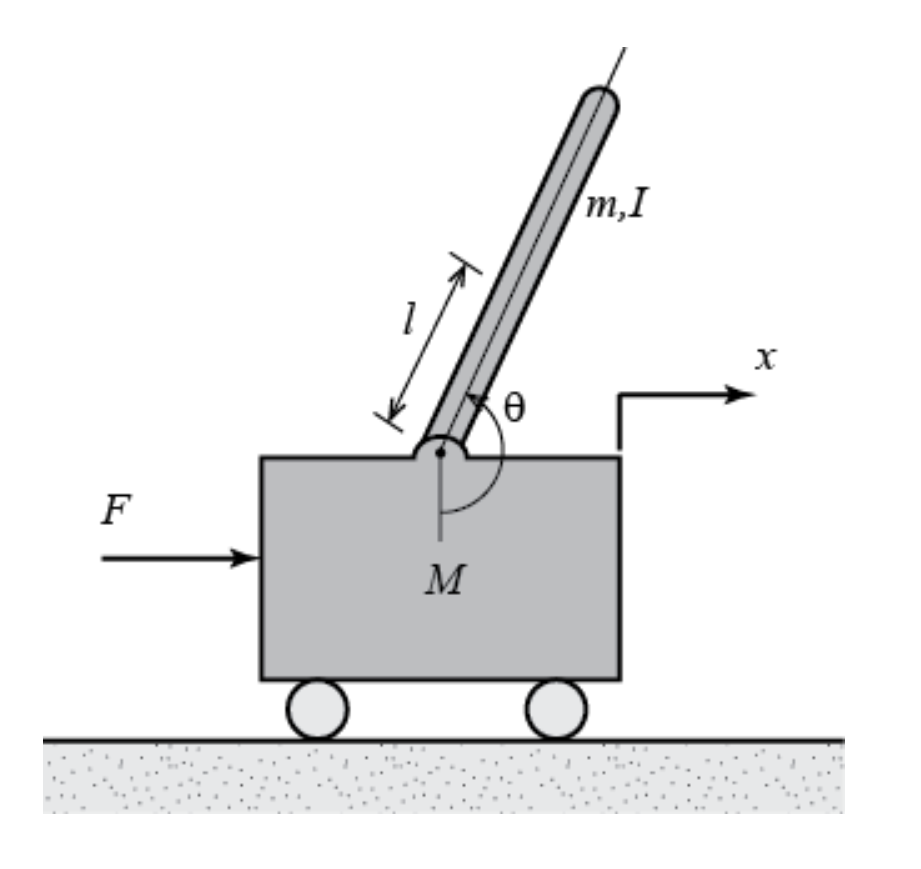
\includegraphics[scale=0.48]{pendulo.PNG}
\end{figure}

\subsection{Análisis diagrama de cuerpo libre y sistema de ecuaciones}

El diagrama de cuerpo libre se presenta en la Figura~\ref{cuerpo}.\\

\begin{figure}[]
\caption{Diagrama de cuerpo libre del péndulo invertido.\label{cuerpo}}
  \centering
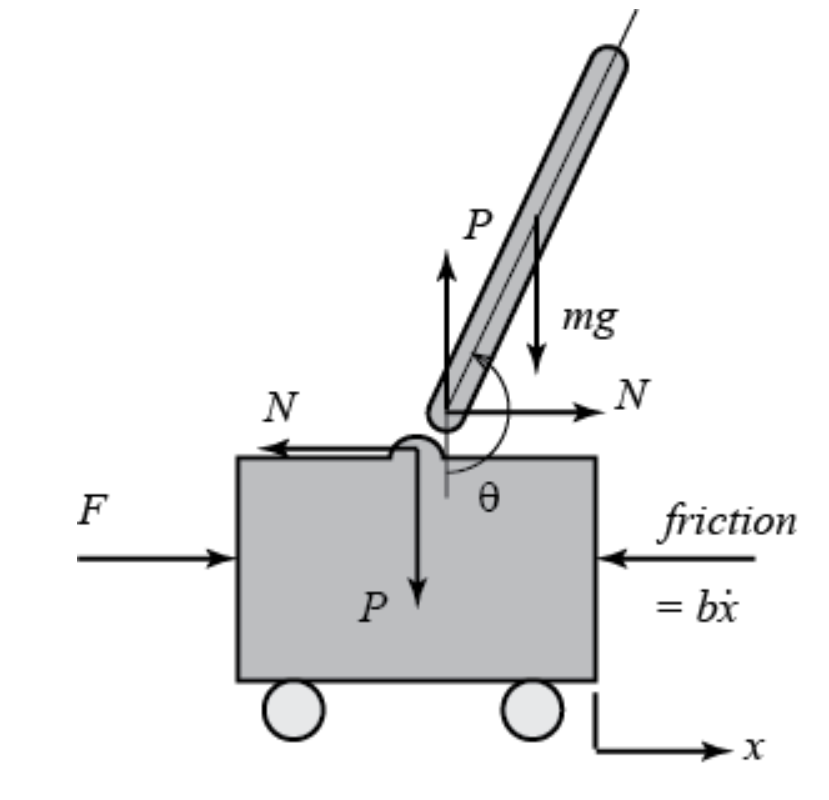
\includegraphics[scale=0.48]{diagrama_cuerpo.PNG}
\end{figure}

Sumando las fuerzas horizontales se obtiene la siguiente ecuación de movimiento
\begin{equation}
\label{eq:motion}
M\ddot{x}+b\dot{x}+N = F
\end{equation}
donde
\[N = m\ddot{x} + ml\ddot{\theta}\cos(\theta) - ml{\dot(\theta)}^2\sin(\theta)\]
generada de la suma de las fuerzas horizontales en el diagrama de cuerpo libre del péndulo.
\\

Sustituyendo $N$ en la ecuación (1), se obtiene
\begin{equation}
  \label{eq:motion1}
  (M + m)\ddot{x} + b\dot{x} + ml\ddot{\theta}\cos(\theta)
     - ml\dot{\theta}^2\sin(\theta) = F
\end{equation}
\textbf{}

Por otro lado, sumando las fuerzas verticales en el diagrama diagrama de cuerpo libre del péndulo y los momentos alrededor del centroide del péndulo, se obtiene, respectivamente
\[P\sin(\theta) + N\cos(\theta) - mg\sin(\theta)
   = ml\ddot{\theta} + m\ddot{x}\cos(\theta)\]
\[Pl\sin(\theta) - Nl\cos(\theta) = I\ddot{\theta}\]
\\
Remplazando la ecuación de la suma de los momentos en la de la suma de las fuerzas verticales (ecuaciones anteriores), da como resultado
\begin{equation}
\label{eq:motion2}
(I + ml^2)\ddot{\theta} + mgl\sin(\theta) = -ml\ddot{x}\cos(\theta)
\end{equation}
\textbf{}

\section{Sistema no lineal}
%Para definir el modelo matemático que describe el sistema
%del Péndulo invertido nos basaremos en el descrito en~\cite{pag}. En
%la Tabla~\ref{tab: des} se describen los distintos parámetros del sistema.
%En~\cite{pag} encontramos las ecuaciones que gobiernan el sistema.
%Estas ecuaciones debemos llevarlas a una representación
%equivalente que permita hallar la representación equivalente
%en espacio de estado.
Las ecuaciones no lineales que describen el sistema son (\ref{eq:motion1}) y (\ref{eq:motion2}), cuya deducción se presenta en la Sección \ref{sec:descripcion}. Para el análisis de sistemas tanto lineales como no lineales se requiere llevarlo a su espacio de estados. El espacio de estados de un sistema es el conjunto de ecuaciones de primer orden que lo describen.

\subsection{Espacio de estados no lineal}\label{subsub:var}
Debido a que las ecuaciones (\ref{eq:motion1}) y (\ref{eq:motion2}), que caracterizan al sistema son de segundo orden, se definen nuevas variables con el fin de expresar éste en su forma canónica. En el Cuadro \ref{my-label} se muestra la definición de dichas variables. 

\begin{table}[!h]
\centering
\caption{Cambio de variables}
\label{my-label}
\begin{tabular}{@{}cl@{}}
\toprule
 \ \ Variable \ \ & Significado \\ \midrule
  $x_1 = x$       & Posición del carro                   \\
  $x_2 = \dot{x}$ & Velocidad del carro                  \\
  $x_3 = \theta$       & Ángulo del péndulo desde la vertical \\
  $x_4 = \dot{\theta}$ & Velocidad angular del péndulo        \\
  $u = F$       & Fuerza de entrada\\ \bottomrule
\end{tabular}
\end{table}

Al derivar las variables de estado $x_1, x_2, x_3, x_4$, se obtiene $\dot{x_1} = \dot{x} = x_2$, $\dot{x_2} = \ddot{x}$, $\dot{x_3} = \dot{\theta} = x_4$ y $\dot{x_4} = \ddot{\theta}$. Despejando $\ddot{x}$ y $\ddot{\theta}$ de las ecuaciones originales del sistema (\ref{eq:motion1}) y (\ref{eq:motion2}), se llega al sistema de ecuaciones (\ref{eq:sistema}), el cual representa el espacio de estados del sistema no lineal.

\begin{eqnarray}
  \label{eq:sistema}
  \left\{
  \begin{array}{ll}
    f_1 = \displaystyle\dot{x_1} = \displaystyle x_2 \\
    f_2 = \displaystyle\dot{x_2} =
            \displaystyle\frac{(I + ml^2)a + m^2l^2g\sin(x_3)\cos(x_3)}
              {(M + m)(I + ml^2)-m^2l^2\cos^2(x_3)}\\
    f_3 = \displaystyle\dot{x_3} = \displaystyle x_4\\
    f_4 = \dot{x_4} = \displaystyle\frac{-ml\cos(x_3)a - (M + m)mlg\sin(x_3)}
                         {(M + m)(I + ml^2) - m^2l^2\cos^2(x_3)}\\
  \end{array}
  \right.
\end{eqnarray}
donde $a = u-bx_2+mlx_4^2\sin(x_3)$

\subsection{Salidas}
La salida del sistema está representada por dos variables de interés: la distancia ($x_1$) y el ángulo del péndulo sobre la vertical inferior ($x_3$). El sistema de ecuaciones (\ref{eq: salidas}) plasma lo mencionado.  

\begin{eqnarray}
  \label{eq: salidas}
  \left\{
  \begin{array}{ll}
    y_1=x_1\\
    y_2=x_3\\
  \end{array}
  \right.
\end{eqnarray}

\subsection{Diagrama de bloques del sistema}
El modelo del péndulo invertido se implementa en MATLAB y su respectivo diagrama de bloques se enseña en la Figura \ref{sistema}. ``El diagrama de bloques es la representación gráfica del funcionamiento interno de un sistema, el cual se explica mediante bloques y sus respectivas relaciones" \cite{wiki:diagra}. La \textit{fcn} es, simplemente, la implementación del espacio de estados en MATLAB. La asignación de los valores de los parámetros y de las condiciones iniciales se hace por medio de una máscara, debido a la facilidad que brinda en la ejecución de dicha actividad.

\begin{figure}[ht!]
\caption{Diagrama de bloques del sistema.\label{sistema}}
  \centering
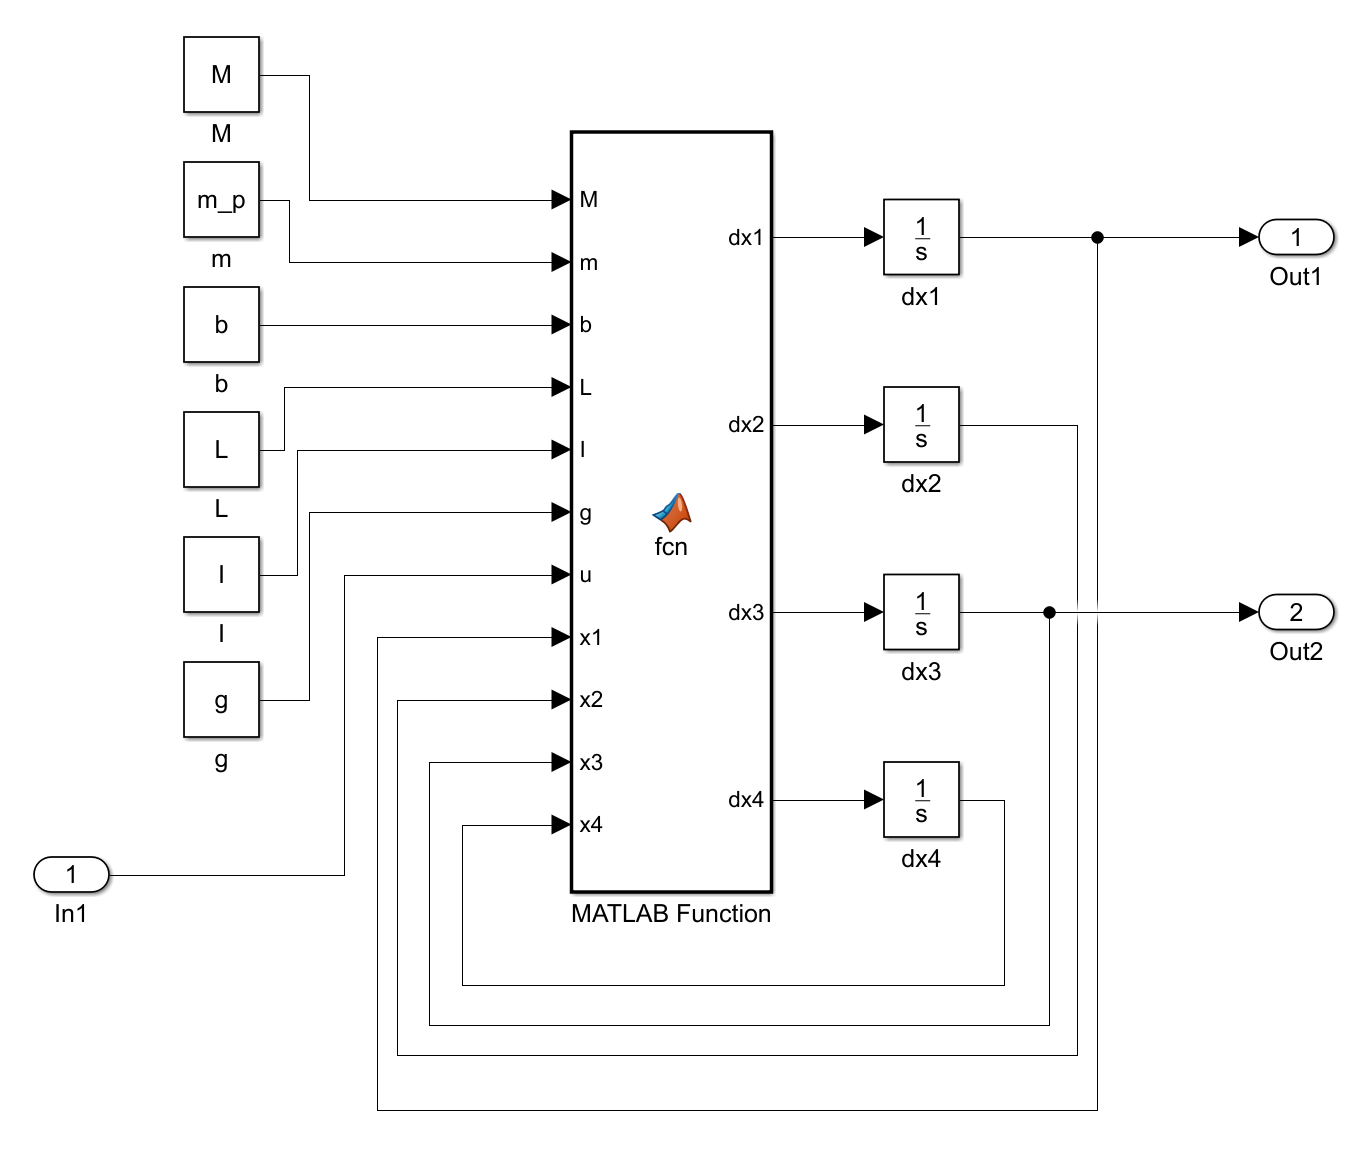
\includegraphics[scale=0.6]{diagrama_bloques_subsistema.PNG}
\end{figure}

\section{Simulación}

A partir de esta sección, las simulaciones que se realizan tienen como parámetros los que se muestran a continuación, a menos que se indique lo contrario: $M=0.5$, $m=0.2$, $b=0.1$, $L=0.3$, $I=0.006$ y $g=9.8$ con unidades señaladas en el Cuadro \ref{tab: des}.

\subsection{Simulaciones con diferentes tipos de entrada}
Al sistema no lineal se le aplican cuatro tipos de entradas: seno, coseno, escalón y sierra. Las respuestas temporales para las salidas se muestran en las Figuras \ref{x1seno}-\ref{x3sierra}. Las características de las señales de entrada son las siguientes:
\begin{itemize}
\item Seno: amplitud=1, fase=0.
\item Coseno: amplitud=1, fase=0.
\item Escalón: unitario con retardo de 5 seg.
\item Sierra: pendiente=1, con repetición cada 25 segundos. 
\end{itemize}
\textbf{}

Al analizar las respuestas temporales, se observa que hay una mayor reacción de las salidas al momento de aplicar la señal de entrada. Para el seno y el coseno esto se nota con mayor claridad al inicio de las respuestas temporales de $x_1$ (ver Figuras \ref{x1seno} y \ref{x1cos}), ya que la señal está activa desde el inicio de la simulación. Siguiendo la idea anterior, se reconoce el momento en que inicia la señal escalón por la perturbación que se presenta en las respuestas temporales de las salidas alrededor del segundo 5 (ver Figuras \ref{x1step} y \ref{x3step}). Exceptuando la respuesta temporal de $x_1$ con entrada coseno, todas las respuestas temporales de $x_1$ tienen un crecimiento promedio positivo. La singularidad mencionada se puede relacionar con la forma de la señal de entrada, la cual comienza con pendiente negativa (decreciendo). Por otro lado, las respuestas temporales de $x_3$ se caracterizan por un comportamiento oscilatorio que podría deberse a la naturaleza de la variable.\\ 

Un análisis por señal se presenta a continuación. 

\subsubsection*{Seno}
Con la función seno, el carro se ve acelerado constantemente y en ambos sentidos ya que la entrada presenta crecimientos y decrecimientos. Esto genera en él un cambio de posición similar a la forma de la función de entrada. Lo anterior se corrobora en la Figura \ref{x1seno}.\\ 

\begin{figure}[ht!]
\caption{Respuesta temporal $x_1$ con señal seno.\label{x1seno}}
  \centering
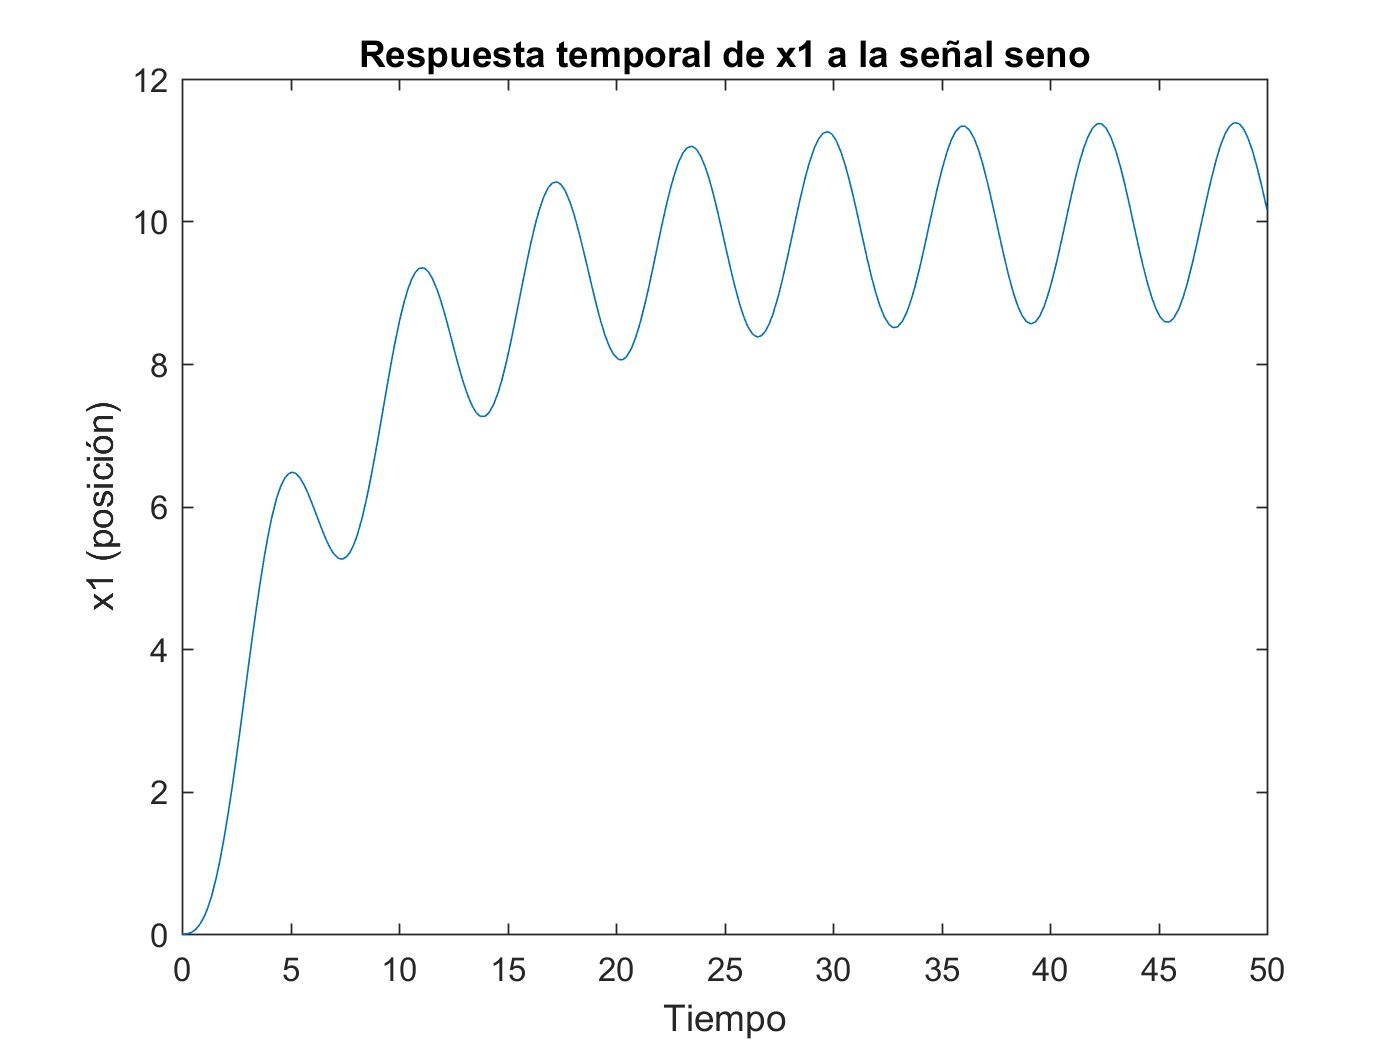
\includegraphics[scale=0.18]{figures/x1seno.png}
\end{figure}

\begin{figure}[ht!]
\caption{Respuesta temporal $x_3$ con señal seno.\label{x3seno}}
  \centering
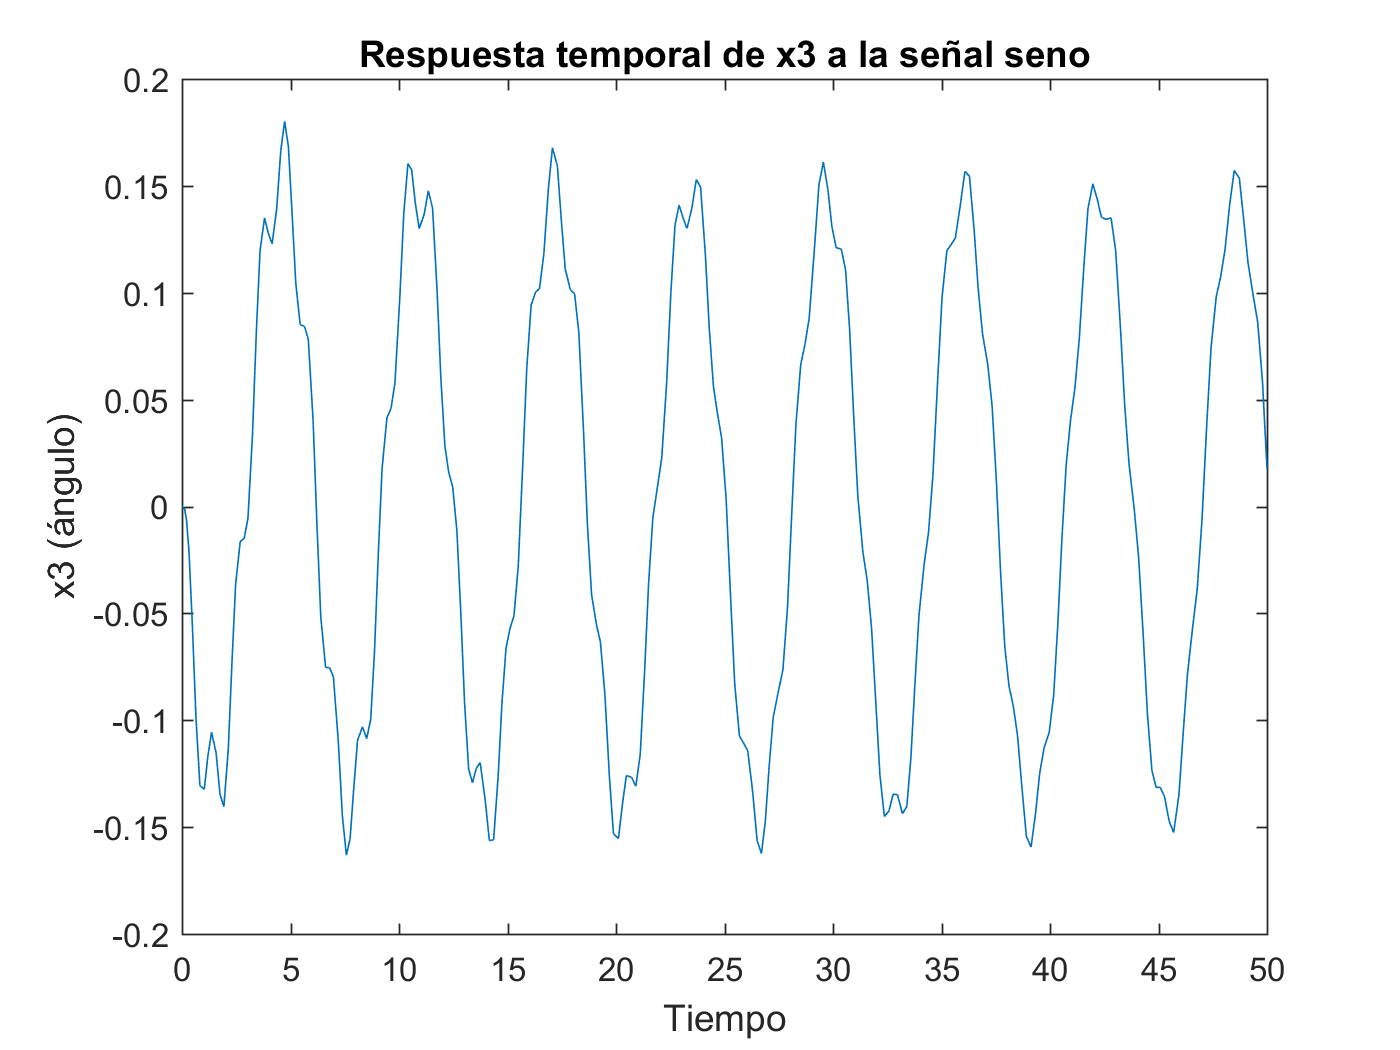
\includegraphics[scale=0.18]{figures/x3seno.png}
\end{figure}

\subsubsection*{Coseno}
El comportamiento del carro con entrada coseno sigue un patrón parecido al del seno, lo cual es esperado por la similitud en la forma funcional de ambas entradas. Sin embargo, al analizar las señales de salida, éstas son diferentes, sobre todo en que una tiende en promedio a decrecer, contrario a lo que ocurre con la otra.\\

\begin{figure}[ht!]
\caption{Respuesta temporal $x_1$ con señal coseno.\label{x1cos}}
  \centering
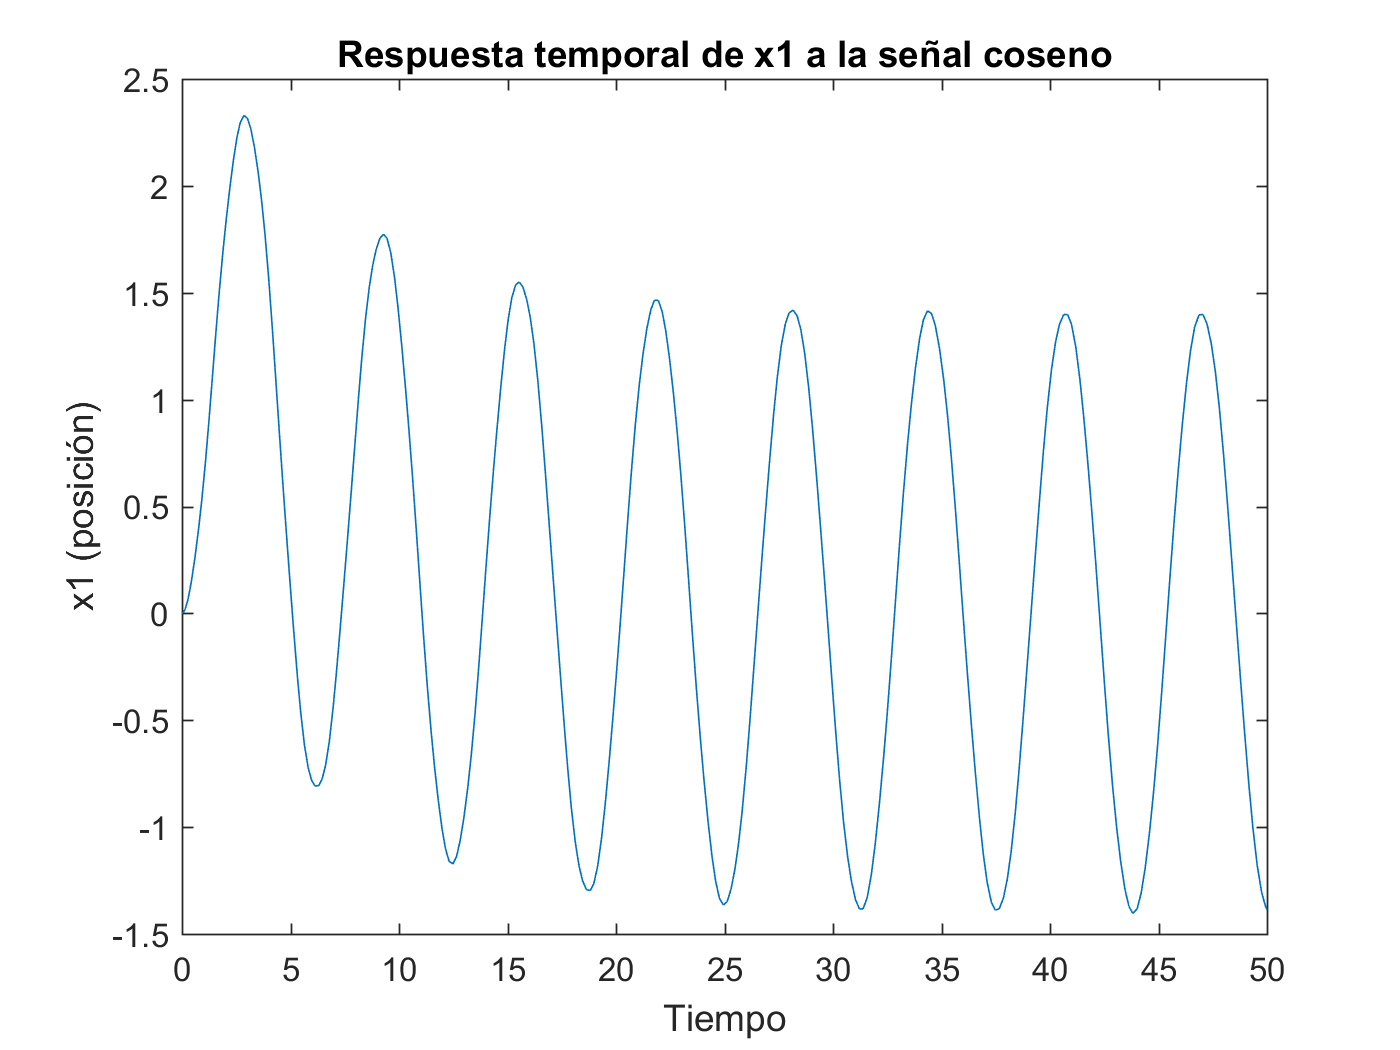
\includegraphics[scale=0.18]{figures/x1cos.png}
\end{figure}

\begin{figure}[ht!]
\caption{Respuesta temporal $x_3$ con señal coseno.\label{x3cos}}
  \centering
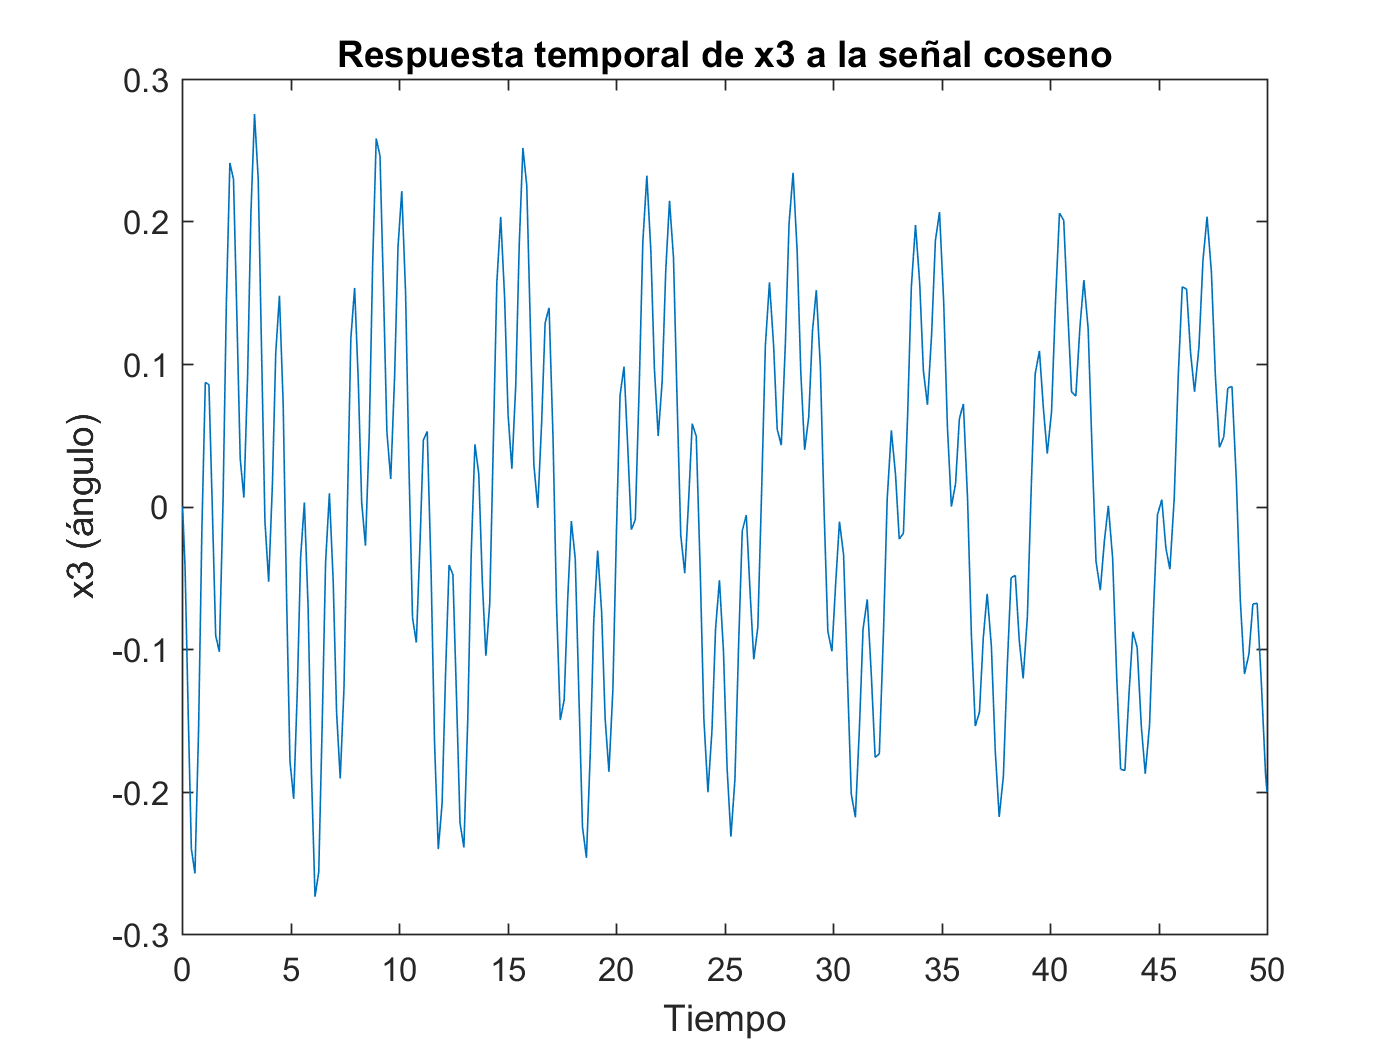
\includegraphics[scale=0.18]{figures/x3cos.png}
\end{figure}

\subsubsection*{Escalón}
Con la función escalón se muestra la variación del sistema ante la aplicación repentina de una fuerza, como ya se mencionó anteriormente. En las Figuras \ref{x1step} y \ref{x3step} puede observarse el comportamiento del sistema ante una fuerza externa nula, antes de que la entrada haga efecto. \\

\begin{figure}[ht!]
\caption{Respuesta temporal $x_1$ con señal escalón.\label{x1step}}
  \centering
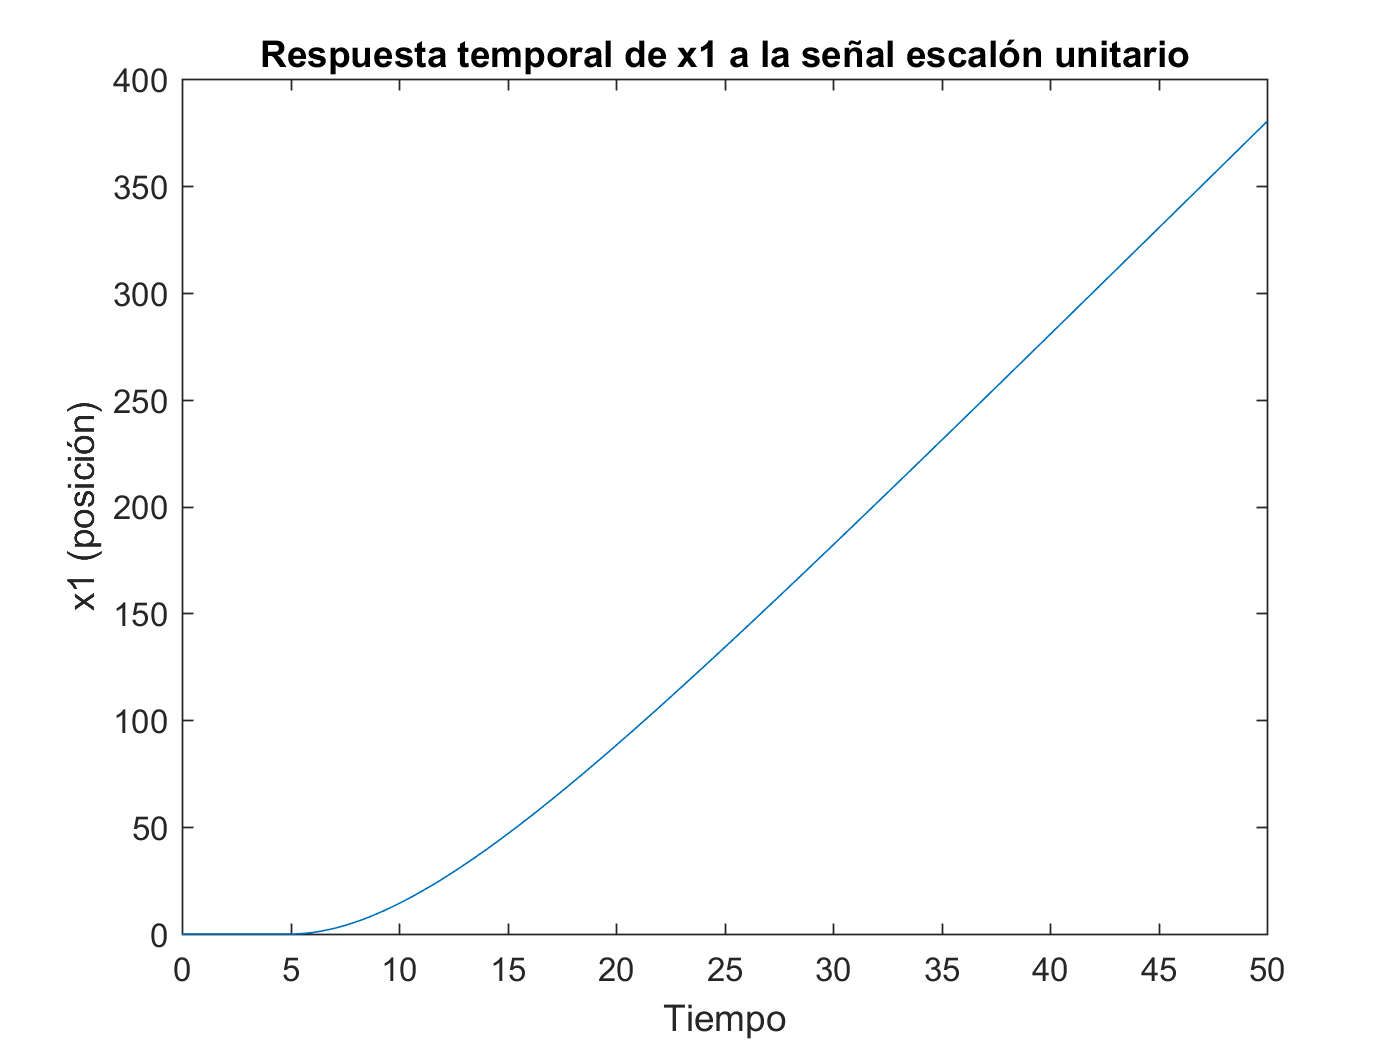
\includegraphics[scale=0.18]{figures/x1step.png}
\end{figure}

\begin{figure}[ht!]
\caption{Respuesta temporal $x_3$ con señal escalón.\label{x3step}}
  \centering
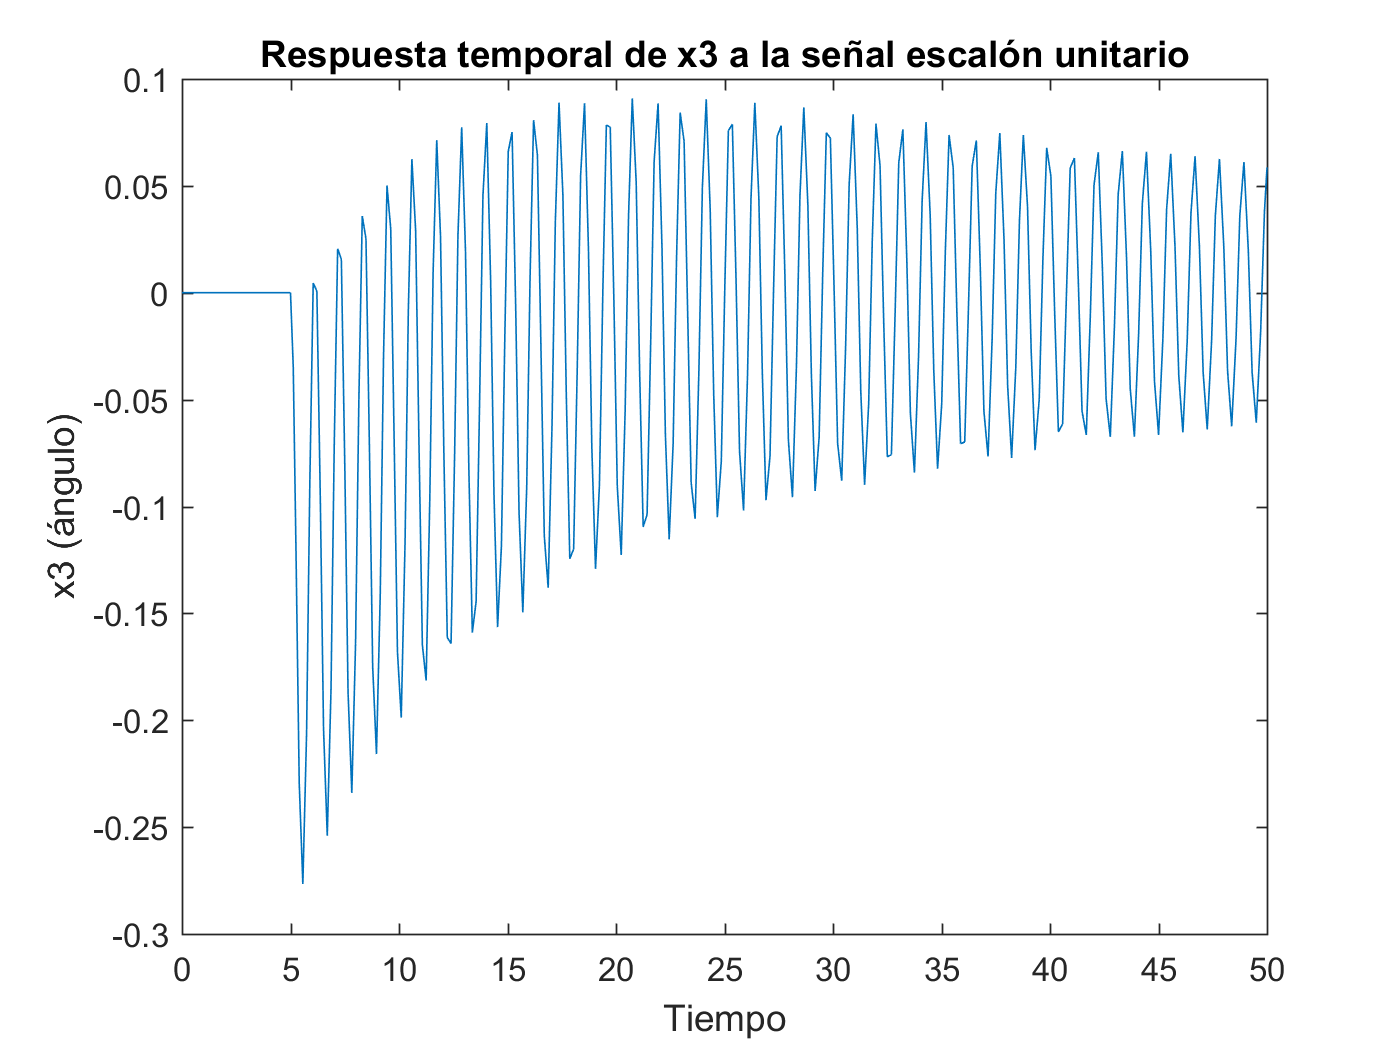
\includegraphics[scale=0.18]{figures/x3step.png}
\end{figure}

\subsubsection*{Sierra}
Con la función sierra se tiene un comportamiento bastante particular, y al igual que la función escalón, es fácil ver el lugar de la discontinuidad. Por otro lado, la discontinuidad en esta señal afecta en mayor medida la respuesta temporal, lo que probablemente se explique por la amplitud del salto. El mayor contraste se presenta en la Figura \ref{x3sierra}.\\

\begin{figure}[ht!]
\caption{Respuesta temporal $x_1$ con señal sierra.\label{x1sierra}}
  \centering
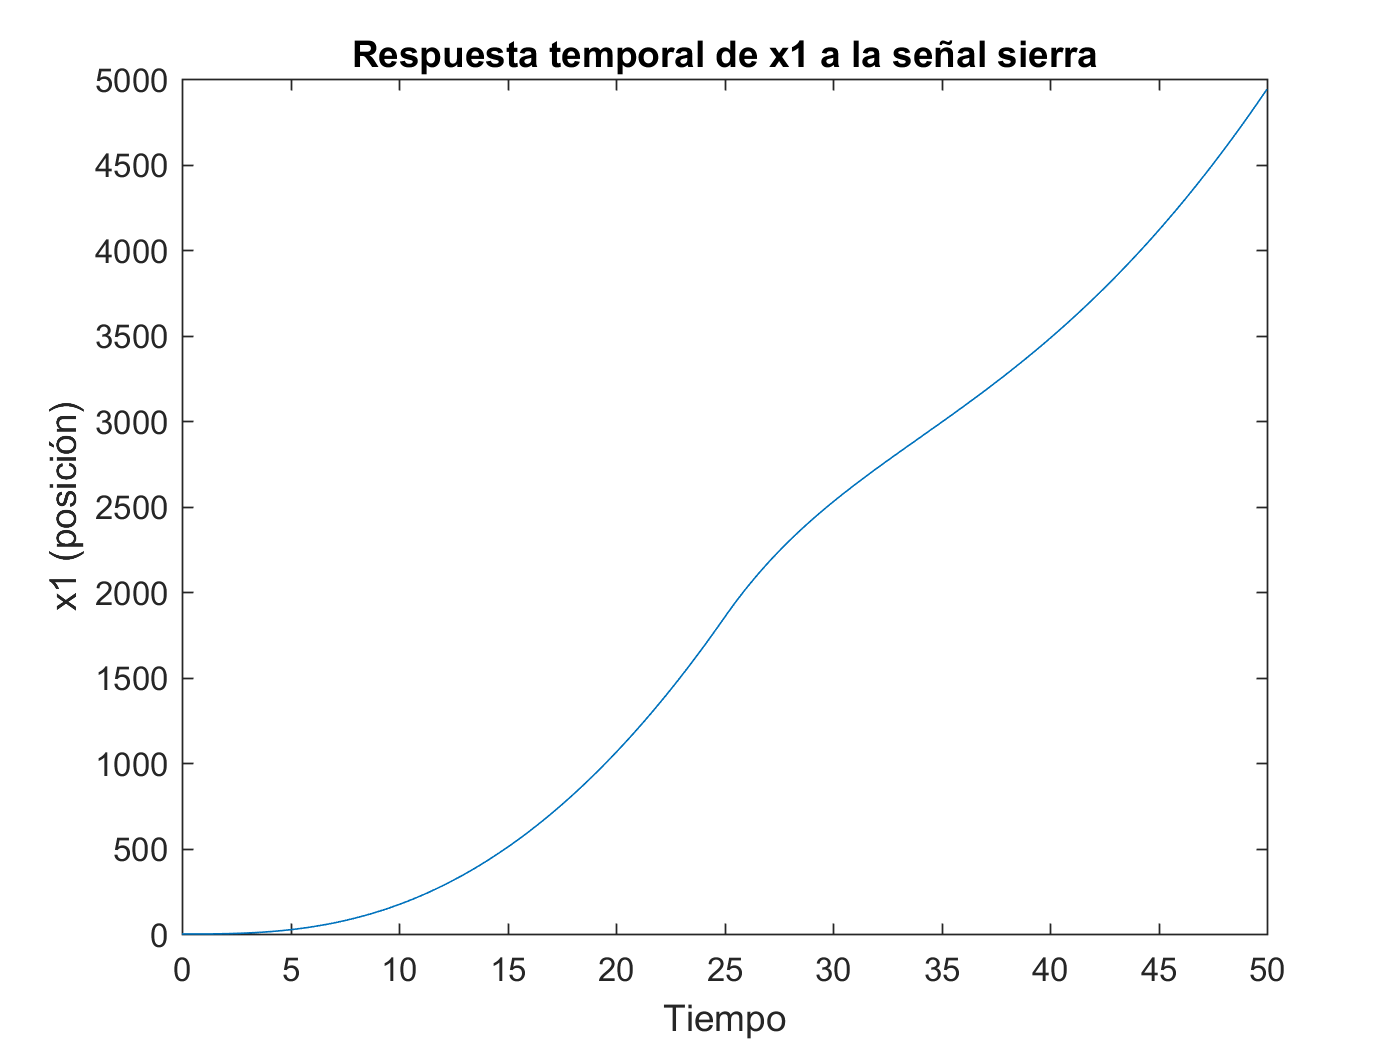
\includegraphics[scale=0.18]{figures/x1sierra.png}
\end{figure}

\begin{figure}[ht!]
\caption{Respuesta temporal $x_3$ con señal sierra.\label{x3sierra}}
  \centering
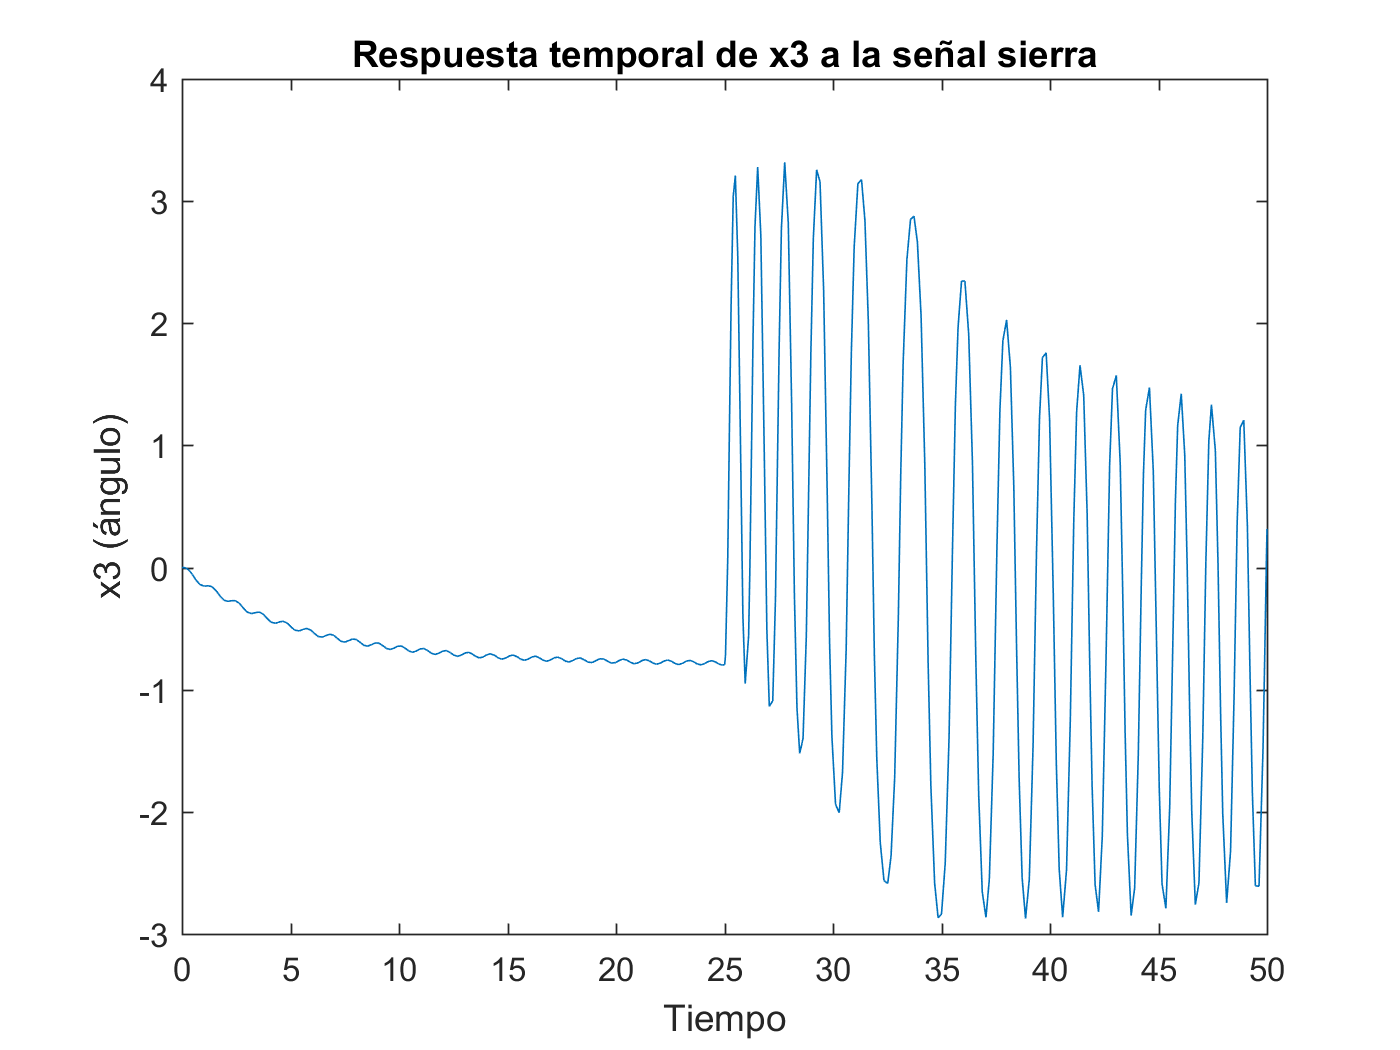
\includegraphics[scale=0.18]{figures/x3sierra.png}
\end{figure}


\subsection{Solución numérica}
La alta complejidad de los sistemas dinámicos, tales como el péndulo invertido, hacen necesario el uso de métodos numéricos para la solución de los mismos. En la presente sección se exponen los métodos numéricos desarrollados para este proyecto con el objetivo de verificar las implementaciones realizadas en \textit{Simulink}. Estos se pueden encontrar en el siguiente repositorio de \href{https://github.com/anpoc/Inverted-pendulum}{GitHub}.\\

\begin{figure}[!h]
\caption{Comparación del método de Euler y Runge Kutta, junto al a la salida de Simulink, escalada, bajo una entrada tipo \textit{step}, con zoom en el intervalo 50-55.\label{fig:nmth}}
  \centering
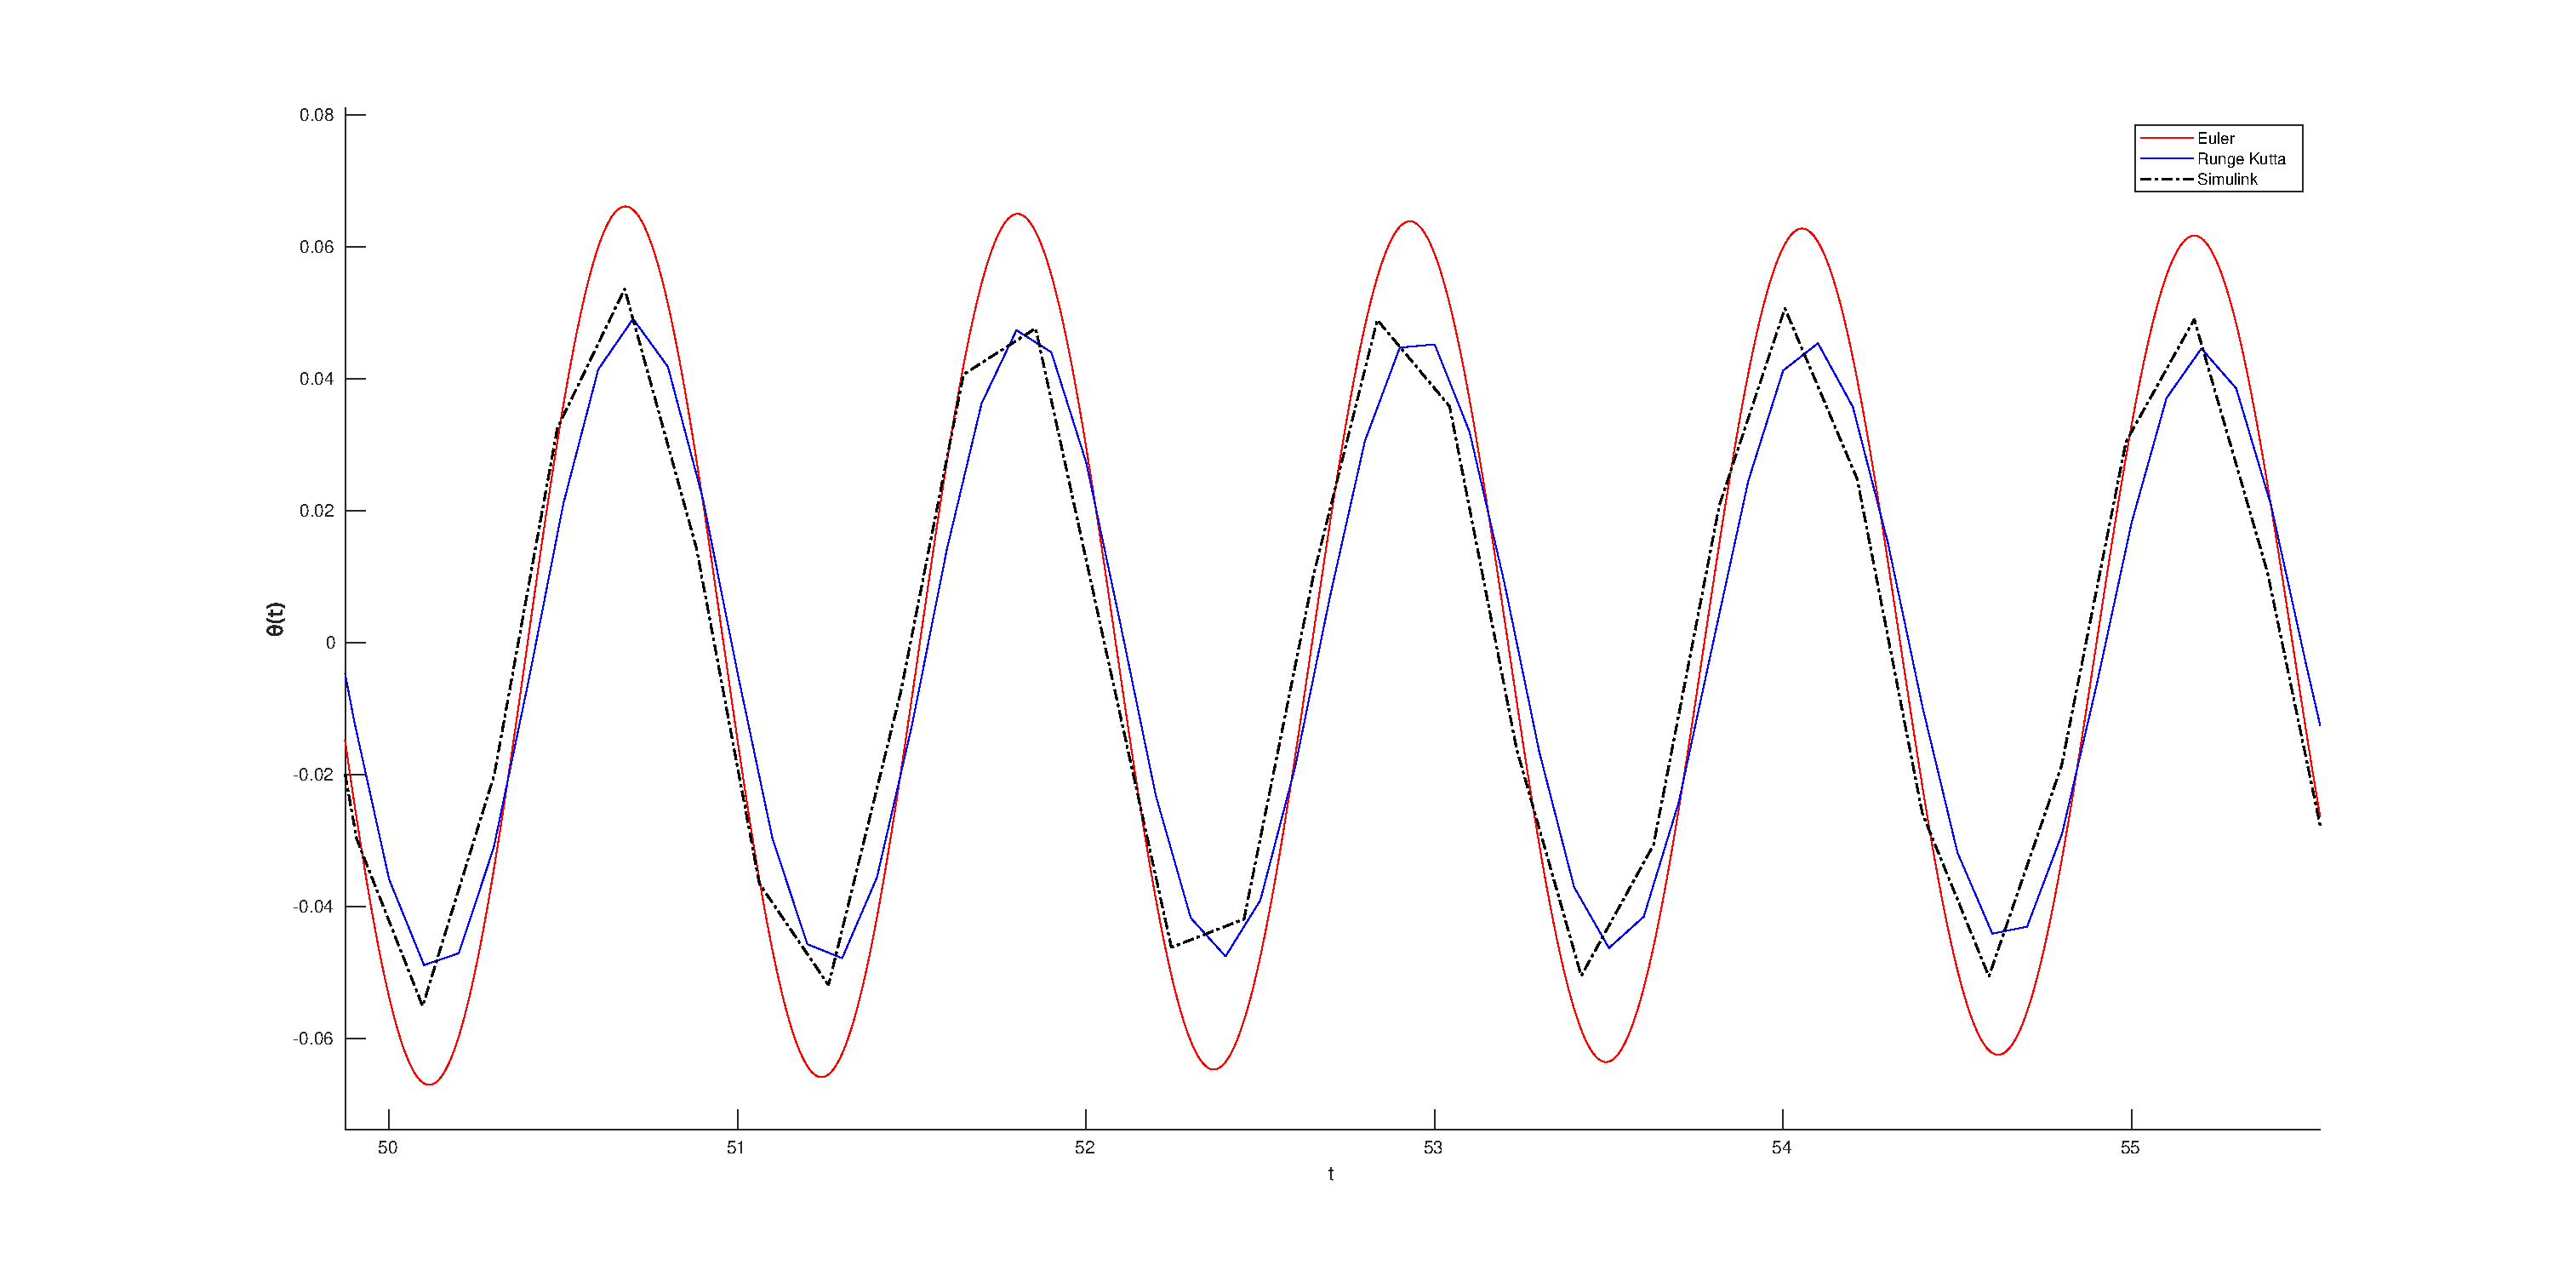
\includegraphics[scale=0.2]{nm.eps}
\end{figure}

\subsubsection*{Método de Euler}
El método de Euler es un procedimiento de integración numérica para resolver ecuaciones diferenciales ordinarias. Éste surge como una aproximación de las Series de Taylor~\cite{eu-1993}. El método consiste en definir un paso \[ h = \frac{x_f - x_0}{n} \] de manera que se obtengan $n + 1$ puntos. A partir de esto, se resuelve de forma recursiva la siguiente ecuación \[ y_n = y_{n - 1} + h f(x_{n - 1}, y_{n - 1}) \] donde $f(x_{n - 1}, y_{n - 1})$ es la derivada en el punto anteriormente obtenido, lo que nos indica la dirección de cambio de la función en dicho punto. Esta pendiente se multiplica por $h$ para obtener el cambio en función del tamaño del paso previamente definido~\cite{eu-1993} (ver~\cite{hamm} para mas información).\\

En la Figura~\ref{fig:nmth} se compara el resultado obtenido en la simulación con el método de Euler, con paso $h = \frac{1}{4000}$, dado que para valores más altos la diferencia entre ambas simulaciones se vuelve bastante notoria. Esta diferencia pueden darse a causa de la alta complejidad de las
ecuaciones de estado, en donde se hace necesario utilizar un
paso muy pequeño. A pesar de lo anterior, aún con un paso diminuto no se consigue una buena aproximación del sistema.\\

\subsubsection*{Método de Runge-Kutta}
El método de Runge-Kutta es un conjunto de procedimientos que permiten la solución numérica de ecuaciones diferenciales. La implementación que se realiza es Runge-Kutta de cuarto orden (RK4). El método RK4 está dado por la siguiente ecuación \[ y_{i + 1} = y_i + \frac{1}{6} h (k_1 + 2 k_2 + 2 k_3 + k_4) \] donde cada valor de $k$ se expresa por
\[
  \begin{cases}
    k_1 = f(x_i, y_i)\\
    k_2 = f(x_i + \frac{1}{2} h, y_i + \frac{1}{2} k_1 h)\\
    k_3 = f(x_i + \frac{1}{2} h, y_i + \frac{1}{2} k_2 h)\\
    k_4 = f(x_1 + h, y_i + k_3 h)
  \end{cases}.
\]
\\
Se observa que cada valor de $k_i$ depende de $k_{i - 1}$ para $i = 2, 3, 4$, lo que nos dice el orden en que estos valores deben calcularse. Adicionalmente, la función $f(x, y)$ hace referencia a la derivada, es decir, $y' = f(x, y)$. (Ver~\cite{hamm} para más información)\\

Para este metodo, el valor del paso es $h = \frac{1}{10}$. La precisión obtenida es tal que en la figura no se logra diferenciar con facilidad la simulación arrojada por \textit{Simulink}.
Esto indica que el método de Runge-Kutta posee un error
suficientemente bajo y ofrece buenas aproximaciones de las ecuaciones de estados. Es importante resaltar que al utilizar un paso relativamente grande,
el tiempo de computo asociado es bajo.\\

\subsection{Sensibilidad paramétrica}
Para analizar la sensibilidad del modelo se considera el efecto del cambio en los parámetros que conforman al mismo, en particular la longitud al centro de masa del péndulo y la masa del péndulo.
Esto ocurre ya que experimentalmente es sencillo y económico reemplazar estas componentes del péndulo. Para realizar las simulaciones se utiliza una entrada \textit{step}.\\

\begin{figure}[t!]
\caption{Respuesta temporal del modelo, ante cambios en el parametro \texttt{L}, la longitud del pendulo, bajo una entrada \texttt{step}, para los valores de $L=1$ (Amarillo),$L=0.5$ (Rojo), $L=0.1$ (Azul)\label{fig:var-len}}
  \centering
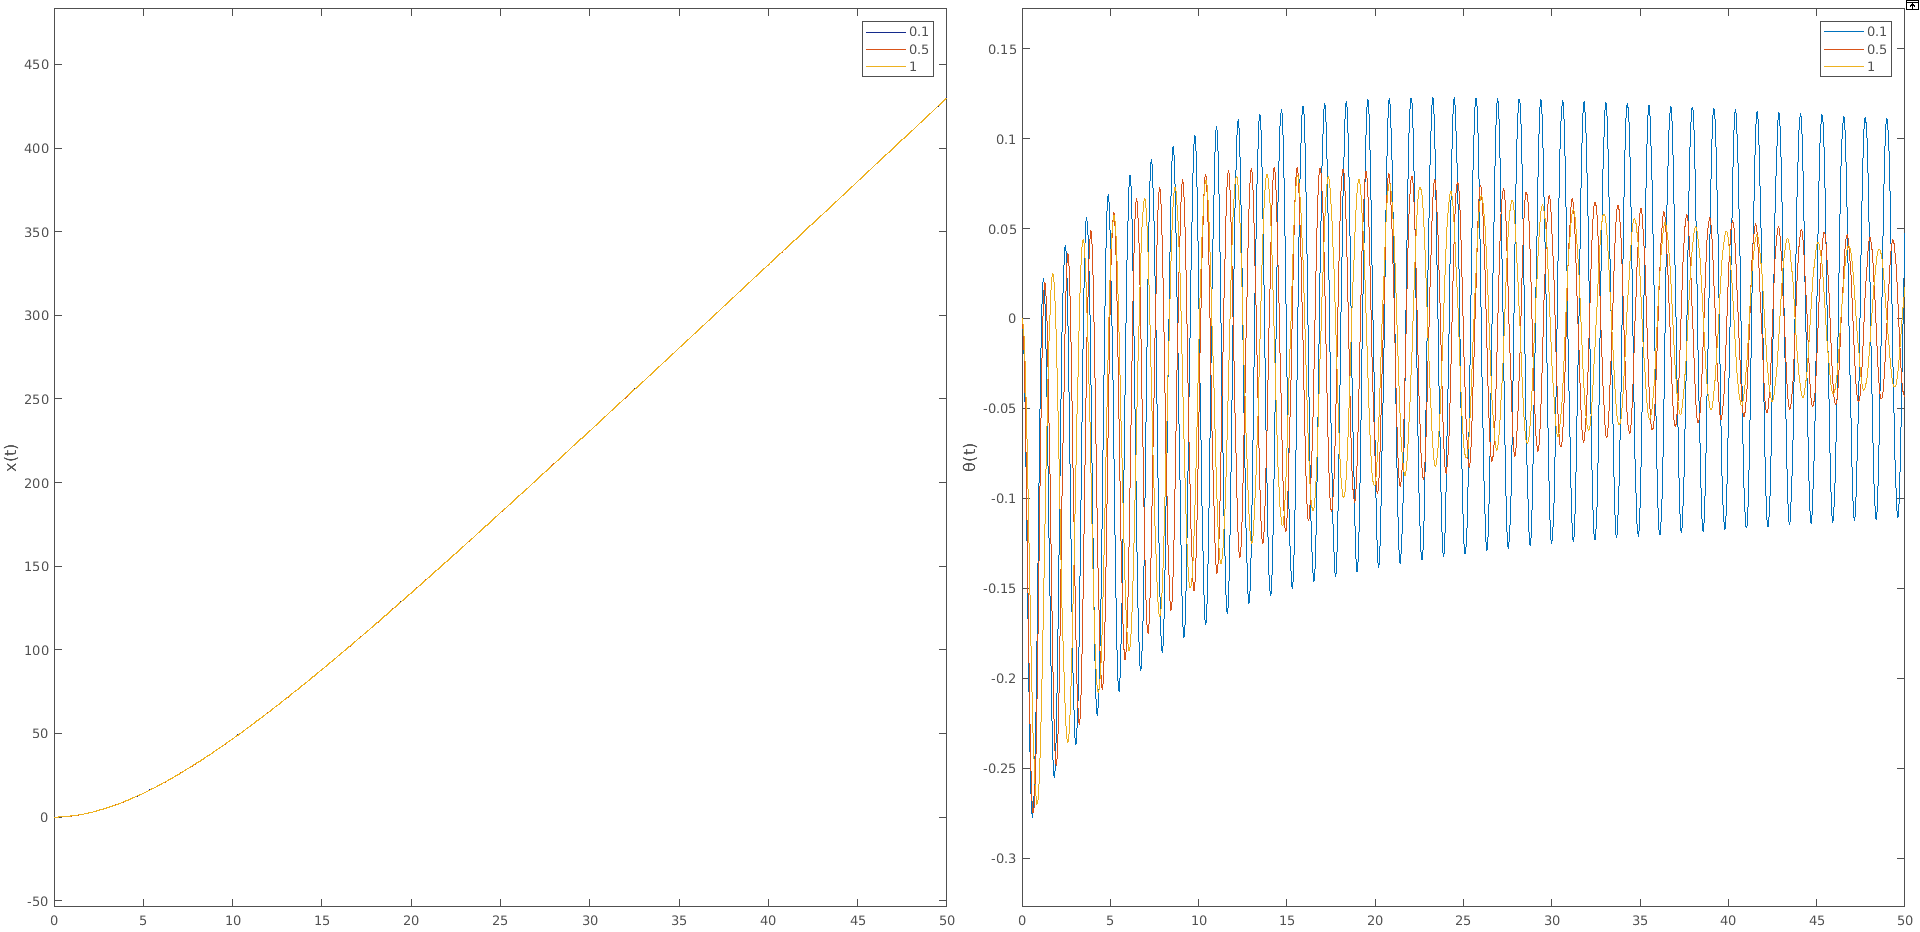
\includegraphics[scale=0.15]{L.png}
\end{figure}

\begin{figure}[t!]
\caption{Respuesta temporal del modelo, ante cambios en el parametro \texttt{m}, la masa del pendulo, bajo una entrada\texttt{step}, para los valores de $m=1$ (Amarillo),$m=0.5$ (Rojo), $m=0.1$ (Azul).\label{fig:var-mass}}
  \centering
	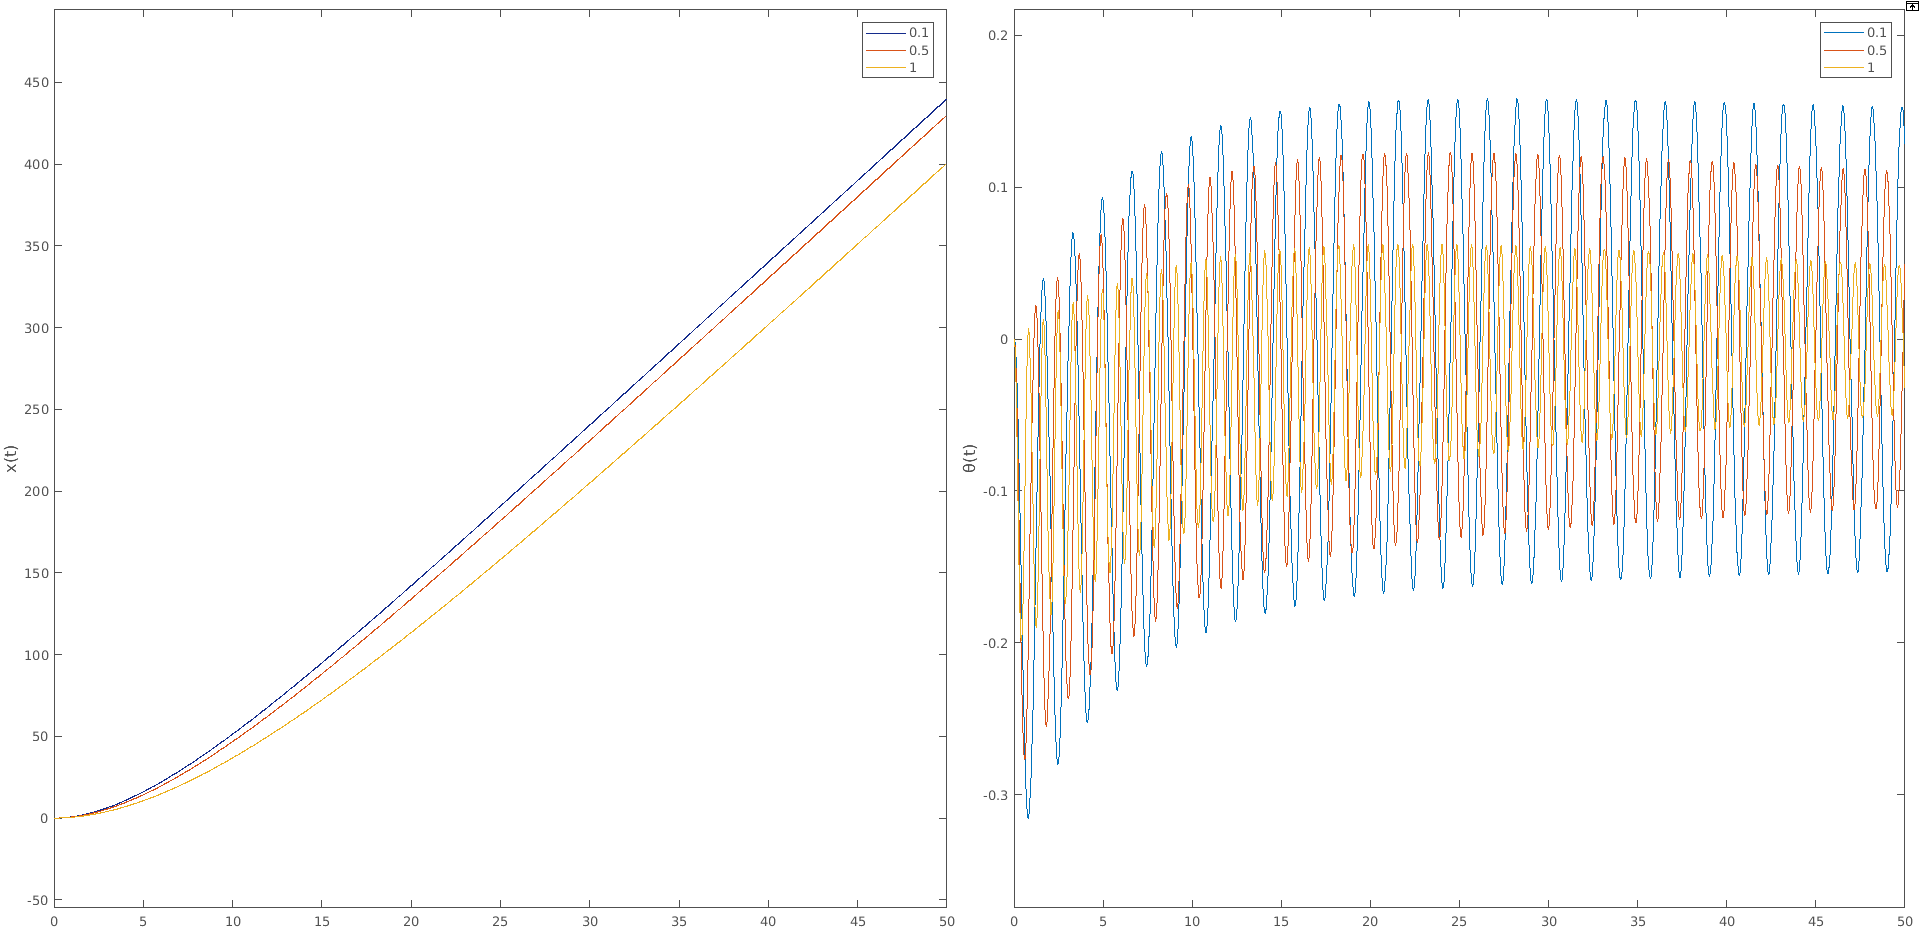
\includegraphics[scale=0.15]{m.png}
\end{figure}

\subsubsection*{Longitud al centro de masa}
En la Figura~\ref{fig:var-len} se varía la distancia del centro de masa
del péndulo. De la gráfica se observa que la amplitud con la que se
mueve el carro disminuye a medida que la distancia del centro
de masa del péndulo también lo hace. Esto ocurre ya que la inercia depende de esta
distancia y es la que provoca dichos movimientos sobre el carro.
Vale la pena resalta que el ángulo del péndulo
no se ve afectado significativamente por esta longitud.\\

\subsubsection*{Masa del péndulo}
En la Figura~\ref{fig:var-mass} se presenta la respuesta temporal
al variar la masa del péndulo, de la cual se observa que la amplitud
del ángulo disminuye a medida que aumenta la masa del mismo. Por otro
lado, la frecuencia con la que éste oscila incrementa, lo cual tiene sentido,
pues el péndulo se mueve más rápido sobre ángulos más pequeños. Lo anterior se
corrobora al ver la gráfica de la posición, la cual no sólo crece más
rápido, sino que lo hace con una mayor concavidad, indicando que la
aceleración del péndulo es mayor y hace que la fuerza requerida
se incremente para poder mover más masa.


\section{Linealización}\label{sec:lin}

Un sistema lineal es de la forma
\[\dot{X}=AX+BU\]
\[Y=CX+DU\]
donde $Y$ es el vector de salidas, $X$ es el vector de estados, $U$ es el vector
de entradas y $A$, $B$, $C$ y $D$ son matrices (o vectores dependiendo de las
dimensiones de $X$ y $U$) de coeficientes constantes.\\

La linealización del modelo del péndulo invertido se realiza tanto analíticamente como por MATLAB utilizando el diagrama de bloques. Dicha linealización, que es una aproximación de un modelo no lineal a uno lineal alrededor de un punto de operación, se desarrolla generalmente en un punto de equilibrio. Para este caso, dicho punto es \[\begin{bmatrix}
x_1 & x_2 & x_3 & x_4 & u
\end{bmatrix}^T=0\]

Los puntos de equilibrio de un sistema se hallan igualando las $f_n$ a 0. Para el sistema en cuestión, se obtienen seis puntos de equilibrio, los cuales se muestran en el Cuadro \ref{tab: ptoseq}.


\begin{table}[ht!]
  \centering
  \caption{Puntos de equilibrio}\label{tab: ptoseq}
  \begin{tabular}{c|c|c|c|c|c|c}
    \hline
     & 1 & 2 & 3 & 4 & 5 & 6\\
    \hline
     $x_1$ & 0 & 0 & 0 & 0 & 0 & 0\\
     $x_2$ & 0 & 0 & 0 & 0 & 0 & 0\\
     $x_3$ & $- \pi + 1.4049i$ &  $-1.4049i$ & $1.4049i$ & $\pi$ & 0 & $\pi+1.4049i$\\
     $x_4$ & 0 & 0 & 0 & 0 & 0 & 0\\
     $u$ & $6.0807i$ & $- 6.0807i$ & $6.0807i$ & 0 & 0 & $- 6.0807i$\\ \hline
\end{tabular}
\end{table}



\subsection{Linealización analítica}
La linealización analítica del sistema se hace por series de Taylor, como se muestra a continuación, con punto de evaluación $X_0$ y $U_0$ el punto de equilibrio indicado anteriormente.
\[\begin{split}
f_i(X, U) \approx f_i(X_0, U_0) + \sum_{j=1}^{4}\frac{\partial f_i(X, U)}{\partial x_j}\bigg\rvert_{X=X_0, U=U_0}\Delta x_j \\
+\frac{\partial f_i(X, U)}{\partial U}\bigg\rvert_{X=X_0, U=U_0}\Delta U
\end{split}\]
\[\begin{split}
y_k(X, U) \approx h_k(X_0, U_0) + \sum_{j=1}^{4}\frac{\partial h_k(X, U)}{\partial x_j}\bigg\rvert_{X=X_0, U=U_0}\Delta x_j\\
+ \frac{\partial h_k(X, U)}{\partial U}\bigg\rvert_{X=X_0, U=U_0}\Delta U
\end{split}\]
donde $i=1,...,4$ y $k=1,2$.\\

Se sabe que las funciones evaluadas en el punto de equilibrio, es decir, $f_i(X_0, U_0)$ y $y_k(X_0, U_0)$, tienden a cero.\\

La representación matricial de la aproximación por series de Taylor para el modelo del péndulo invertido se muestra a continuación.
\begin{eqnarray}
\Delta\dot{X} = A\Delta X + B\Delta U\\
\Delta Y = C\Delta X + D\Delta U
\end{eqnarray}
donde
\[A =\begin{bmatrix}
    0 & 1 & 0 & 0\\
    0 & -2/11 & 147/55 & 0\\
    0 & 0 & 0 & 1\\
    0 & 5/11 & -343/11 & 0
\end{bmatrix}
\]
\[B = \begin{bmatrix}
    0 &
    20/11 &
    0 &
    -50/11
\end{bmatrix}^{T}\]
\[C = \begin{bmatrix}
    1 & 0 & 0 & 0\\
    0 & 0 & 1 & 0
\end{bmatrix}\]
\[D = \begin{bmatrix}
    0&
    0
\end{bmatrix}^{T}\]

\subsubsection{Linealización con Simulink}
Con base en el modelo de bloques mostrado en la Figura \ref{sistema} y utilizando la función \textit{linmod} de MATLAB, se obtiene la siguiente linealización del modelo.

\[A =\begin{bmatrix}
    0 & 0 & 1 & 0\\
    0 & 0 & 0 & 1\\
    0 & 2.6727 & -0.1818 & 0\\
    0 & -31.1818 & 0.4545 & 0
\end{bmatrix}
\]
\[B = \begin{bmatrix}
    0 &
    0 &
    1.8182 &
    -4.5455
\end{bmatrix}^{T}\]
\[C = \begin{bmatrix}
    1 & 0 & 0 & 0\\
    0 & 1 & 0 & 0
\end{bmatrix}\]
\[D = \begin{bmatrix}
    0&
    0
\end{bmatrix}^{T}\]

Se observa que las posiciones de las variables $x_2$ y $x_3$ se encuentran trocadas. Al hacer la respectiva transformación lineal, usando la matriz $T$ que se define abajo, se evidencia que la linealización analítica y la linealización utilizando Simulink son equivalentes.

\[T=\begin{bmatrix}
1 & 0 & 0 & 0\\
0 & 0 & 1 & 0\\
0 & 1 & 0 & 0\\
0 & 0 & 0 & 1
\end{bmatrix}\], 

\subsection{Estabilidad en el punto de equilibrio $X_0=0$, $U_0=0$}
La estabilidad en el punto de equilibrio se infiere de los valores propios de la matriz $A$ del sistema linealizado. Los valores propios se calculan así 
$$\det(A-\lambda I)=0$$ 
En MATLAB esto se puede hacer por medio del comando \textit{eye}. Con base en dichos valores, que se muestran en el Cuadro \ref{valores propios}, y teniendo cuenta que todos son negativos y existe uno de ellos en cero, el punto de equilibrio estudiado es críticamente estable.

\begin{table}[!h]
\centering
\label{valores propios}
\caption{Valores propios de la matriz A}
\begin{tabular}{ccl}
$\lambda_1$ & = & $0$\\
$\lambda_2$ & = & $-0.1429 + 0.0000i$\\
$\lambda_3$ & = & $-0.0195 + 5.5835i$\\
$\lambda_4$ & = & $-0.0195 - 5.5835i$\\
\end{tabular}
\end{table}

\subsection{Curva de linealidad para la variable $x_3$}
La curva de linealidad obtenida enviando entradas $u \in [-5;5]$ al modelo lineal y al no lineal se muestra en la Figura \ref{fig:curve}. La curva azul hace referencia a los resultados del modelo no lineal, mientras la naranja al modelo lineal. Para entradas $u \in [-2.5; 2.5]$ se considera que el modelo lineal representa una buena aproximación del modelo no lineal ya que se presentan errores absolutos menores a 0.02.\\

\begin{figure}[!h]
\caption{Curva de linealidad para la variable $x_3$ con entradas $u \in [-5;5]$ con tiempo de corrida 300s.\label{fig:curve}}
  \centering
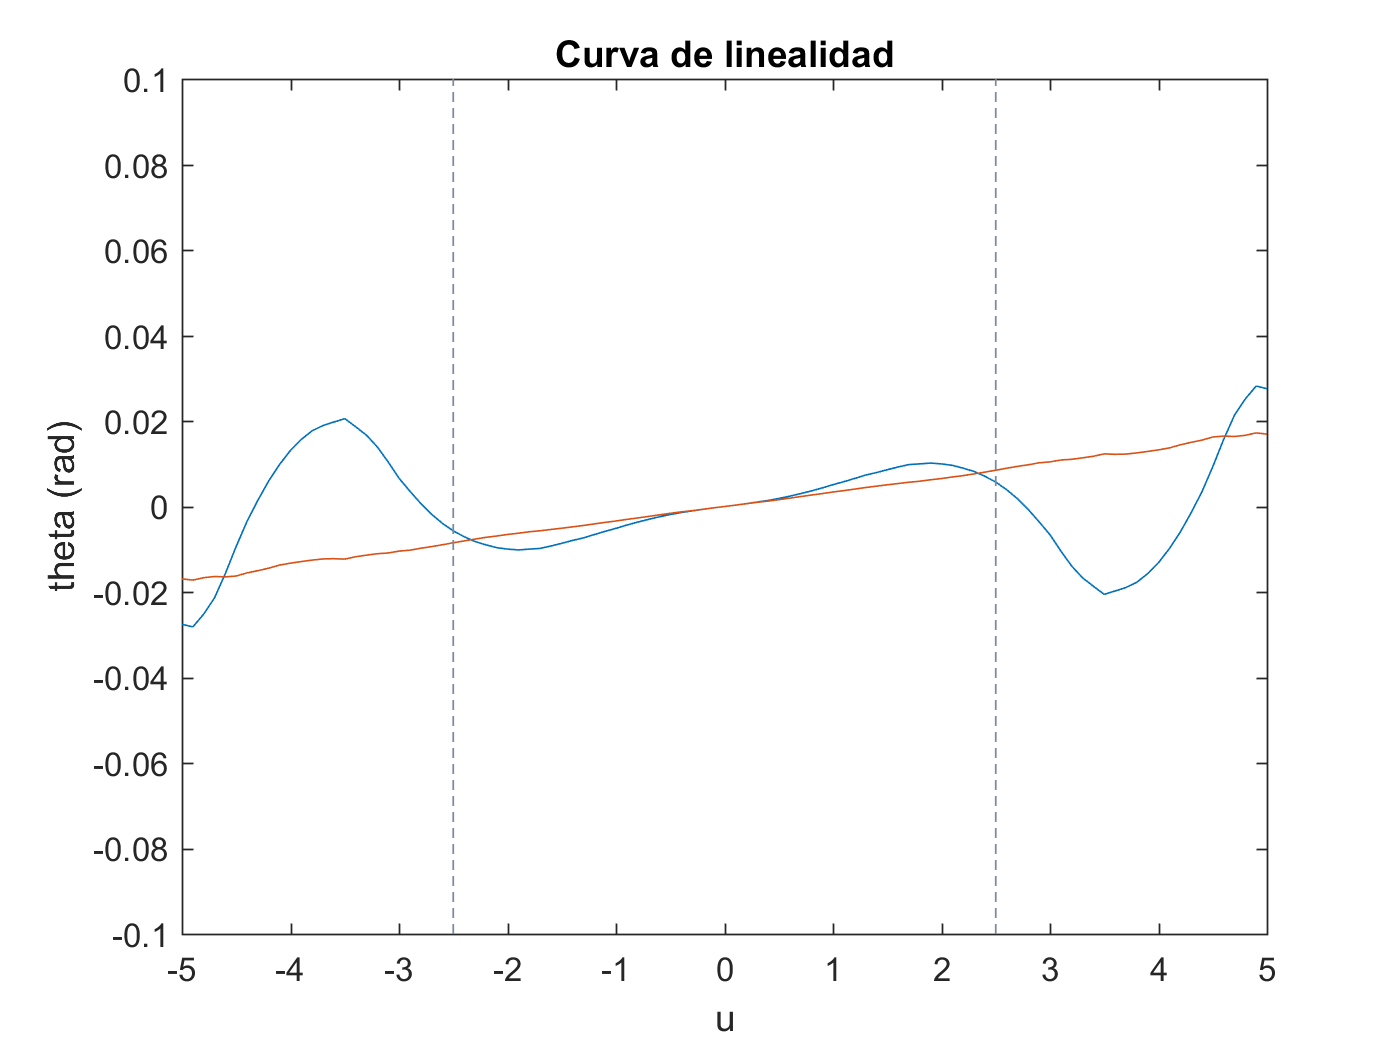
\includegraphics[scale=0.2]{curva_lin.png}
\end{figure}
       
\subsubsection{Curva de linealidad con \textit{Step}}
Otra forma de hallar la curva de linealidad es por medio de una señal escalera. Para una escalera con vector de amplitud $[-5.0; -4.9;...;4.9;5]$ y paso cada 5000s, teniendo un tiempo total de simulación de 500000s, se genera la curva de linealidad mostrada en la Figura \ref{fig:curve_s}. Nuevamente, la curva azul hace referencia a los resultados del modelo no lineal, mientras la naranja al modelo lineal.\\

\begin{figure}[h!]
\caption{Curva de linealidad para la variable $x_3$ con señal escalera y tiempo de corrida 500000s.\label{fig:curve_s}}
  \centering
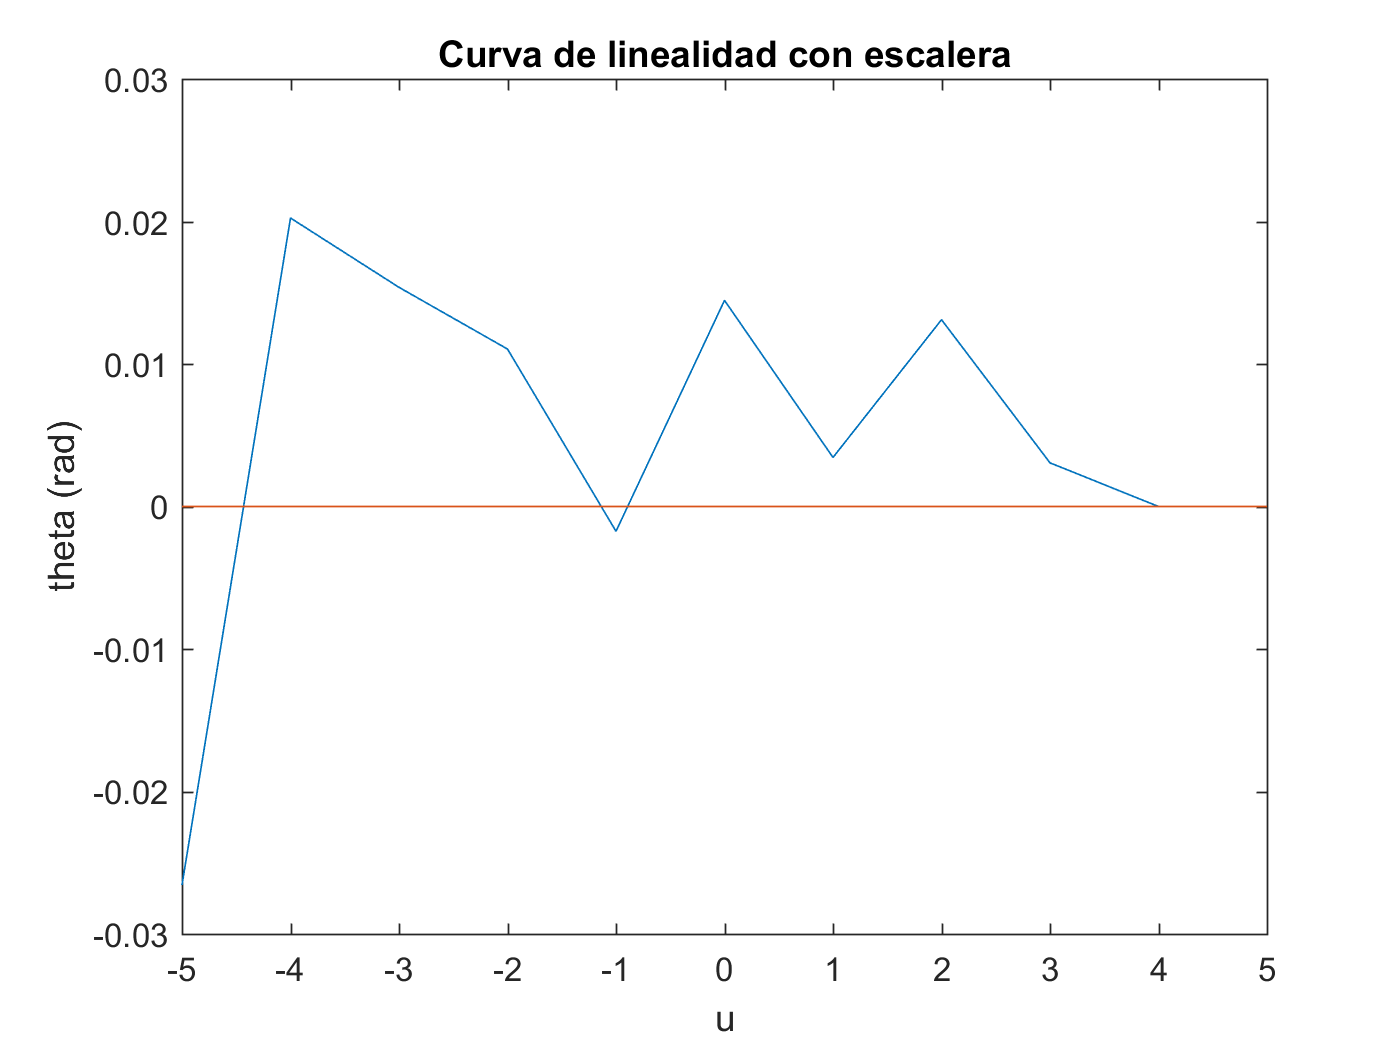
\includegraphics[scale=0.2]{curva_lin_esc.png}
\end{figure}
       
Se observa una similitud entre ambas curvas de linealidad, pero claramente la obtenida mediante la señal escalera no logra ser una aproximación lo suficientemente buena. Esto se puede deber principalmente a que el sistema no se alcanza a estabilizar antes de que la entrada le mande la siguiente señal o a que se trata de hacer la aproximación a una señal continua a partir de un conjunto de puntos discretos y el tamaño del conjunto de puntos puede no ser el adecuado, es decir, la distancia entre los puntos puede ser relativamente grande. Esto último se verifica al ver que la curva azul no es suave.

\section{Variación de entradas y condiciones iniciales: Modelo lineas vs. modelo no lineal}

\subsection{Variación de entrada dentro del rango de linealidad}

Se sabe que el rango de linealidad, es decir, aquel rango en el que el modelo lineal es robusto y es una buena aproximación del modelo no lineal alrededor del punto de equilibrio $X_0=0, U_0=0$, es $[-2.5;2.5]$. Por ende, se eligen dos valores en este rango $u = 0.5$ y $u = -2.0$ y se muestran las gráficas obtenidas para $x_3$ en las Figuras  $\ref{fig:u0.5}$ y $\ref{fig:u-2}$, respectivamente. Ambas figuras muestran la contraposición de las respuestas temporales para $x_3$ del modelo lineal y no lineal. Mas dado que esta diferencia no se observa con claridad, se añade a las gráficas la diferencia entre las respuestas temporales, representado por la curva amarilla. En ambas esta diferencia es muy pequeña, próxima a cero, y con mayores valores al inicio de la simulación. Se cumple que el rango de linealidad supuesto genera resultados esperados, con lo que se concluye que el rango puede ser apropiado.  

\begin{figure}[h!]
\caption{Respuesta temporal variable $x_3$ para entrada $u=0.5$\label{fig:u0.5}}
  \centering
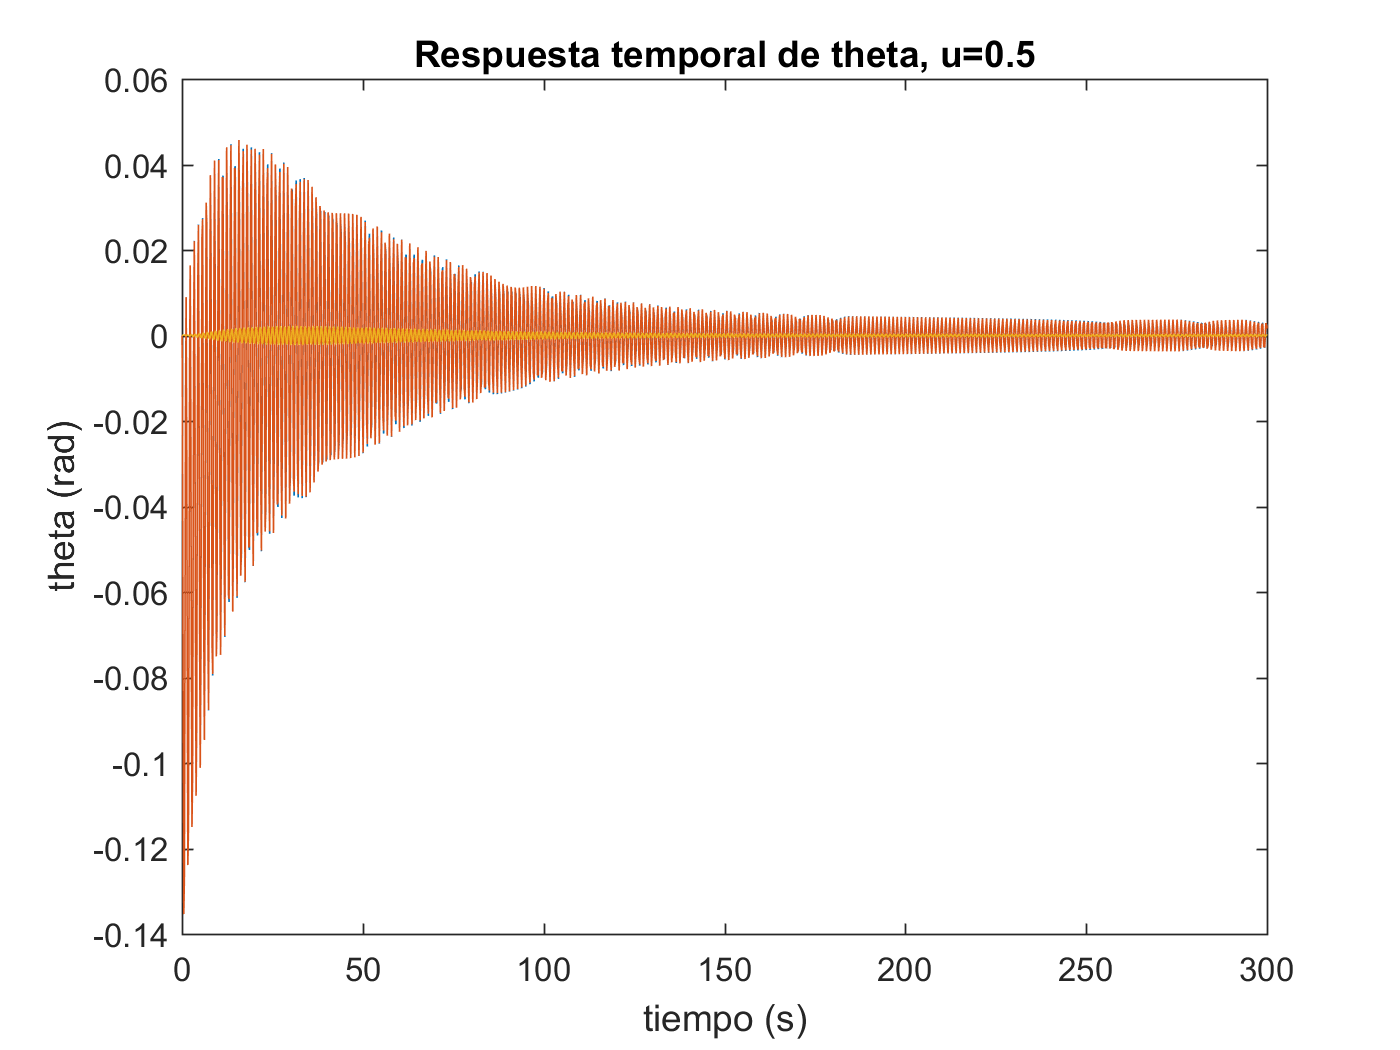
\includegraphics[scale=0.19]{Graficaslvsnl/u0_5.png}
\end{figure}

\begin{figure}[h!]
\caption{Respuesta temporal variable $x_3$ para entrada $u=-2.0$\label{fig:u-2}}
  \centering
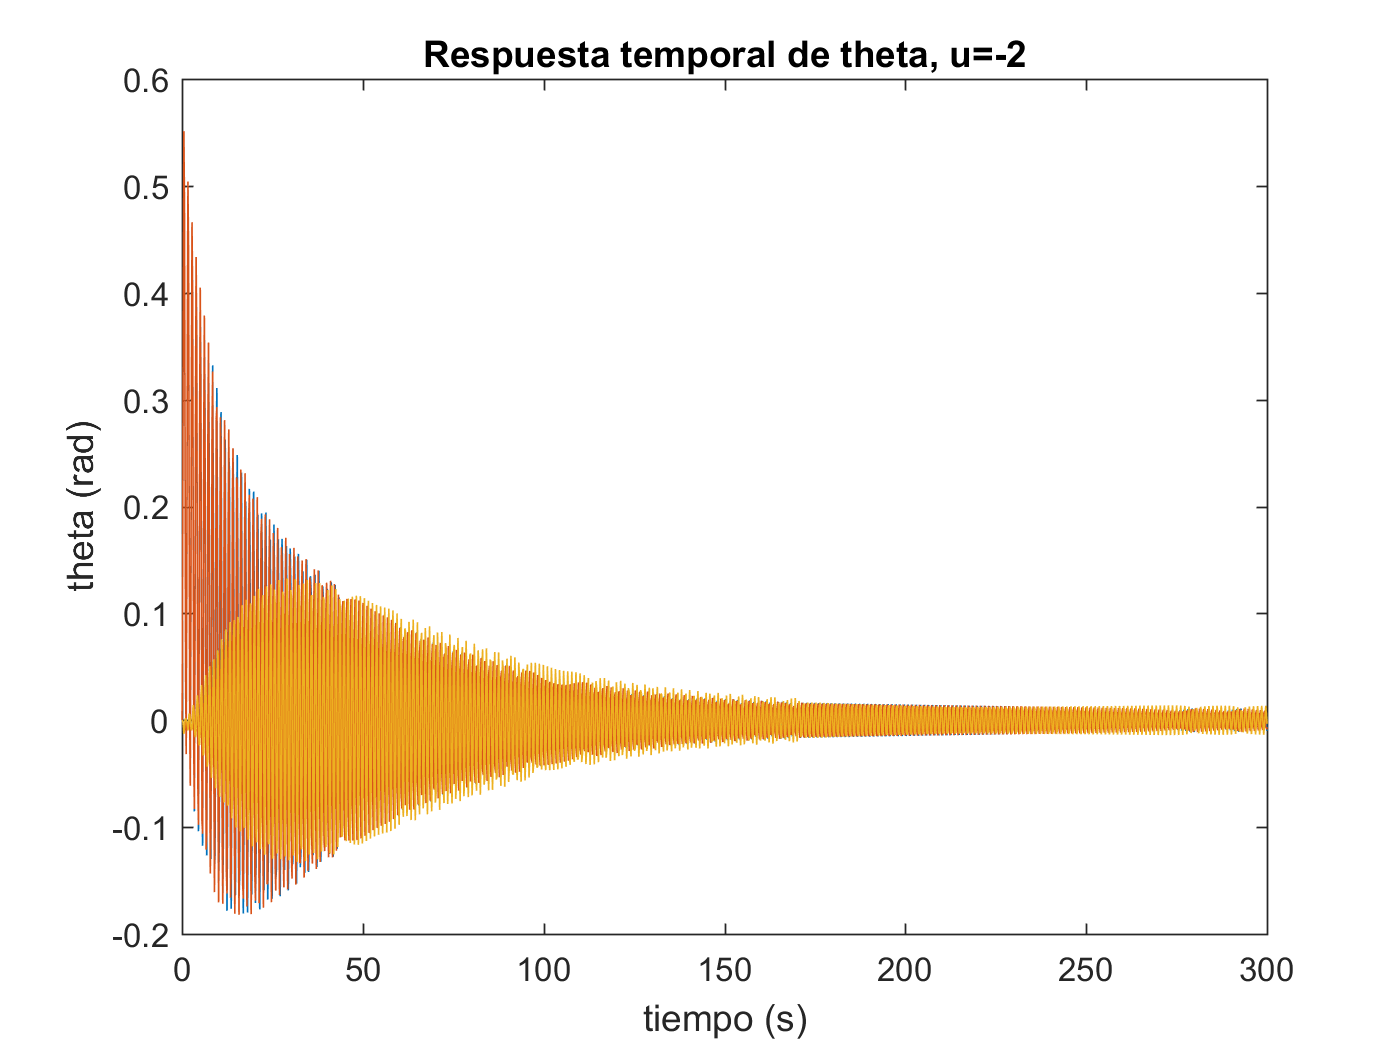
\includegraphics[scale=0.19]{Graficaslvsnl/u-2.png}
\end{figure}
       
\subsection{Variación de entrada fuera del rango de linealidad}
Como se dijo anteriormente, el rango de linealidad elegido es $[-2.5,2.5]$. Se escogen los valores $u=6$ y $u=-100$, por fuera del rango mencionado. En $u=-100$, Figura \ref{fig:u-100}, se observa que el modelo lineal no es una aproximación válida para el modelo no lineal. Por otro lado, para $u=6$, la diferencia en la respuesta temporal obtenida por el modelo lineal y el no lineal no es tan clara como para $u=-100$, a pesar de que se alcanza a ver zonas azules denotando diferencia entre las curvas. Dado lo mencionado anteriormente, se añade la gráfica de contraposición de las respuestas con la diferencia entre ellas, Figura \ref{fig:u6dif}. Esta diferencia no es relativamente grande, con máximo valor absoluto alrededor de 1. Según el valor de relajamiento que se permita en la diferencia entre las respuestas temporales producidas por el modelo lineal y por el no lineal, se puede considerar ampliar el rango de linealidad propuesto.

\begin{figure}[h!]
\caption{Respuesta temporal variable $x_3$ para entrada $u=6.0$\label{fig:u6}}
  \centering
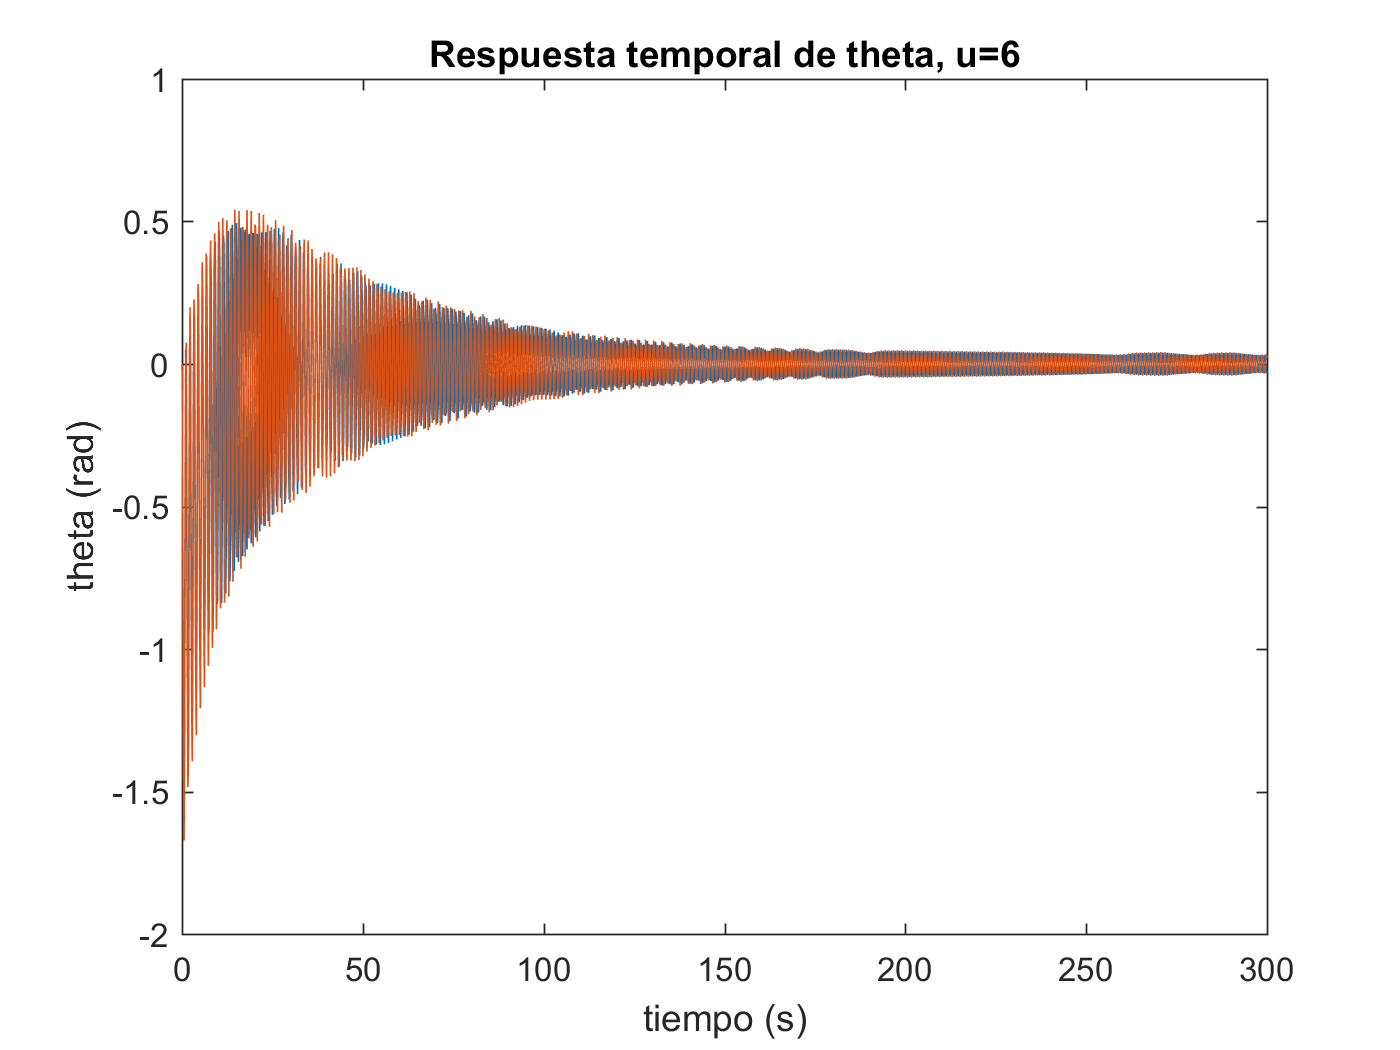
\includegraphics[scale=0.19]{Graficaslvsnl/u6.png}
\end{figure}

\begin{figure}[h!]
\caption{Respuesta temporal variable $x_3$ para entrada $u=6.0$ con diferencia entre las respuestas\label{fig:u6dif}}
  \centering
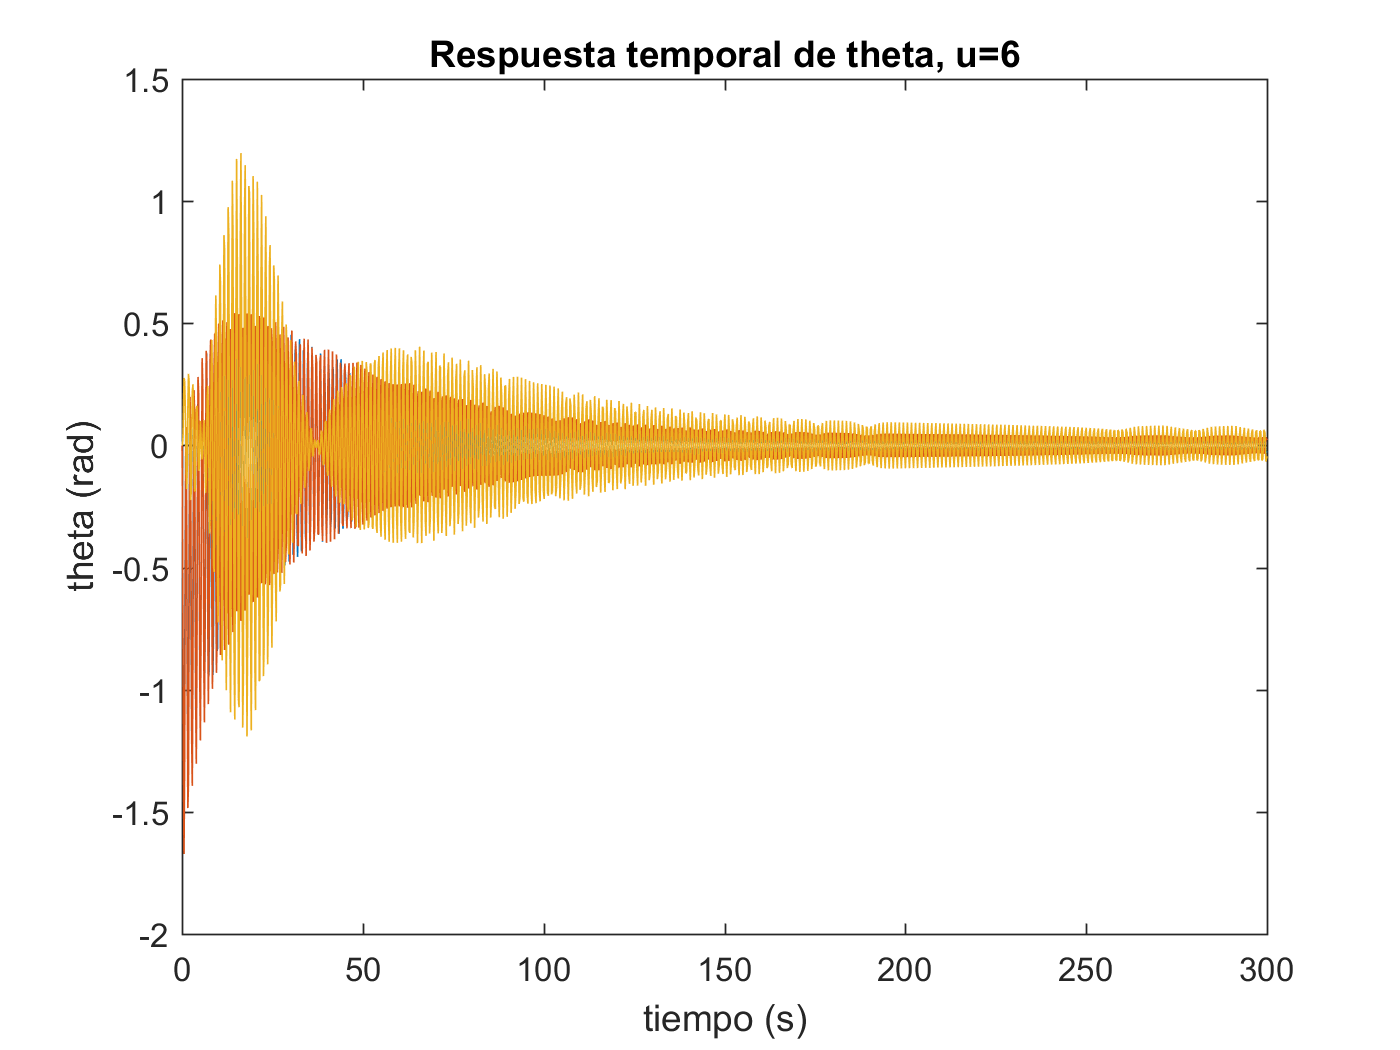
\includegraphics[scale=0.19]{Graficaslvsnl/u6dif.png}
\end{figure}

\begin{figure}[h!]
\caption{Respuesta temporal variable $x_3$ para entrada $u=-100.0$\label{fig:u-100}}
  \centering
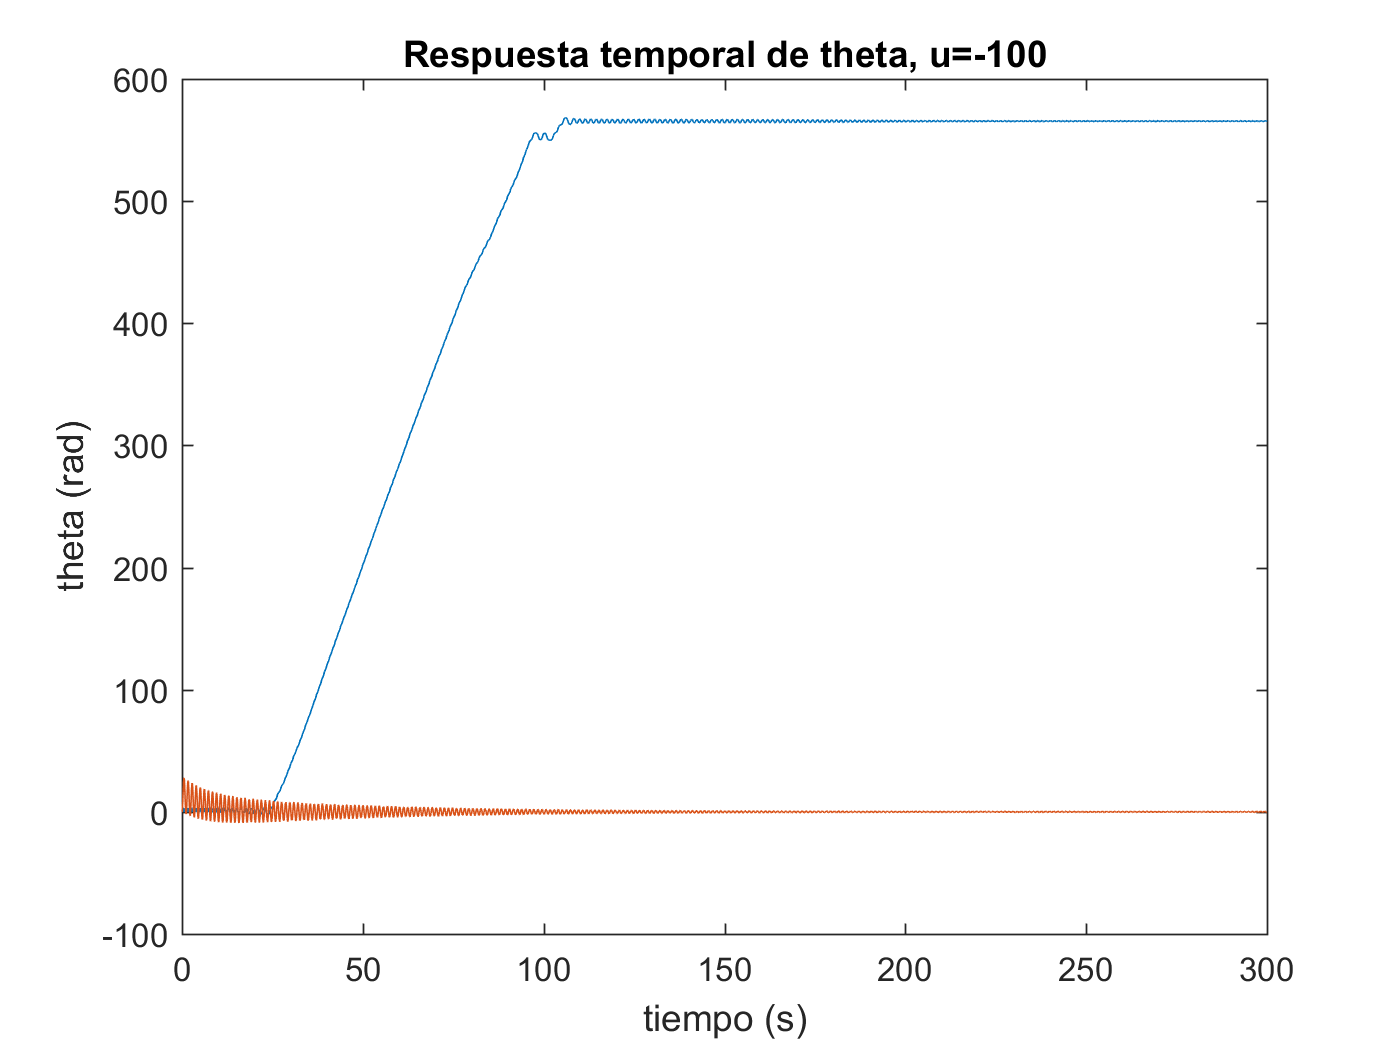
\includegraphics[scale=0.19]{Graficaslvsnl/u-100.png}
\end{figure}
       
\subsection{Variación condiciones iniciales}
Las Figuras \ref{fig:t0.01} y \ref{fig:t0.1} son producidas con pequeñas variaciones de la condición inicial de $x_3$. La Figura \ref{fig:t0.01} corresponde a una variación de 0.01 en la condición inicial y entrada $u=0$. La Figura \ref{fig:t0.1} es obtenida con variación de 0.1 en la condición inicial y entrada $u=0.1$. Comparando las dos gráficas mencionadas anteriormente, se concluye que variaciones relativamente pequeñas en la condición inicial para $x_3$, produce un desplazamiento vertical en la respuesta temporal del modelo lineal, igual al cambio en la condición. Por otro lado, este cambio define el rango de variación inicial en la respuesta temporal para el modelo no lineal. Esto se observa en ambas gráficas. Cuando $u=0$, la gráfica correspondiente al modelo lineal es una línea recta. Por último, cuando se varía $u$ en pequeñas cantidades, se presenta oscilamiento en la respuesta temporal para $x_3$ del modelo lineal.

\begin{figure}[h!]
\caption{Respuesta temporal variable $x_3$ para entrada $u=0$ y condicional inicial $x_{30}=0.01$\label{fig:t0.01}}
  \centering
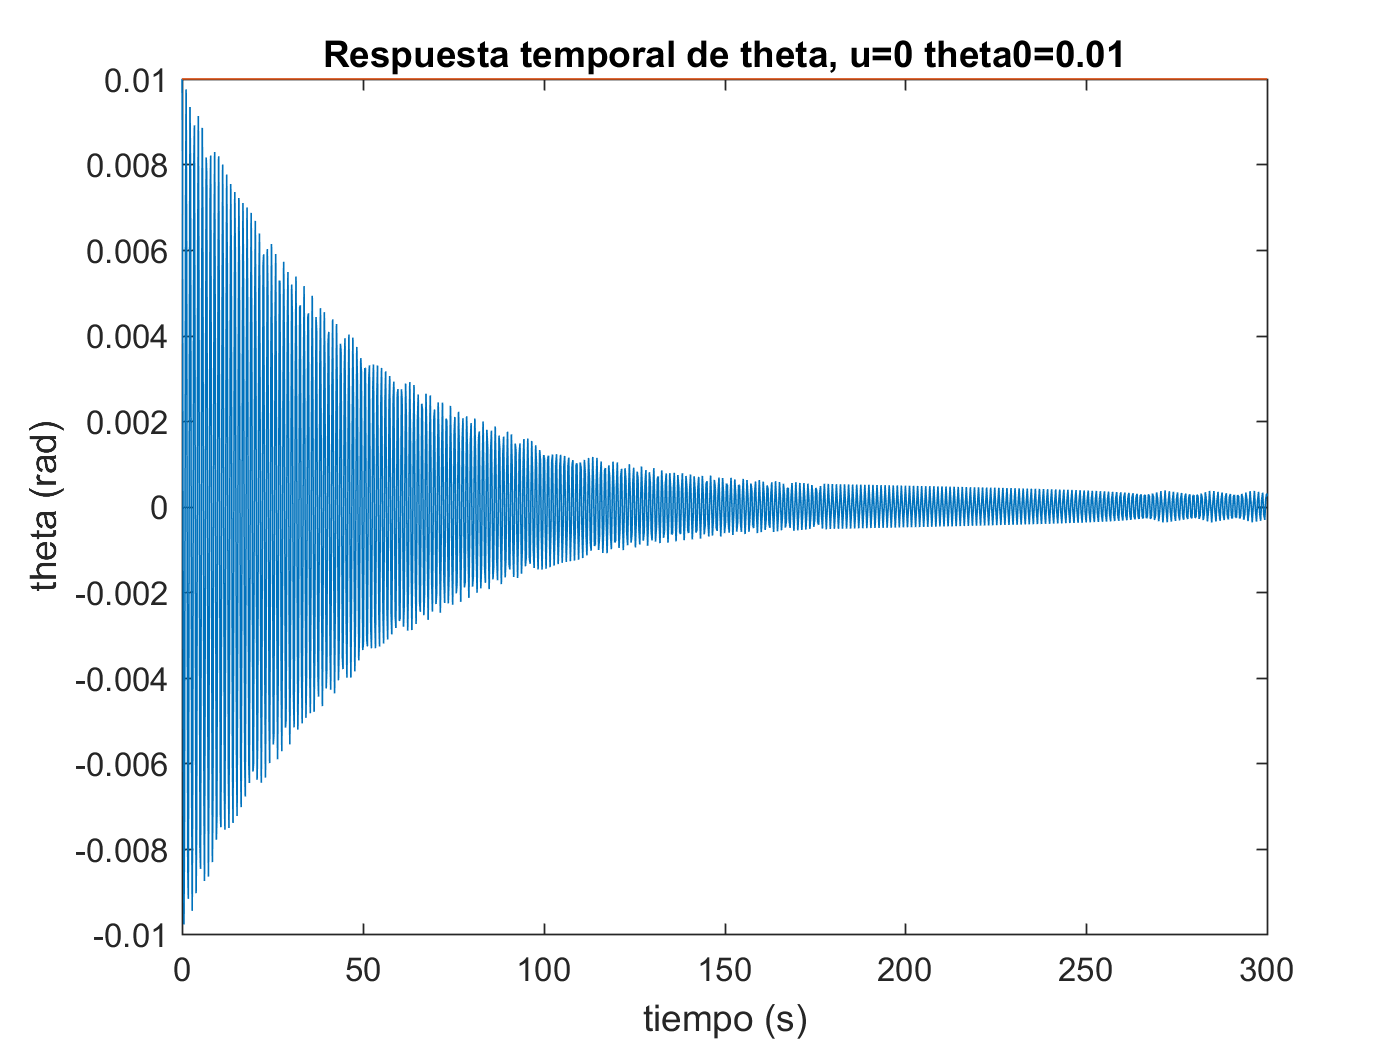
\includegraphics[scale=0.19]{Graficaslvsnl/t0_01.png}
\end{figure}
       
\begin{figure}[h!]
\caption{Respuesta temporal variable para entrada $u=0.1$ y condición inicial $x_{30}=0.1$\label{fig:t0.1}}
  \centering
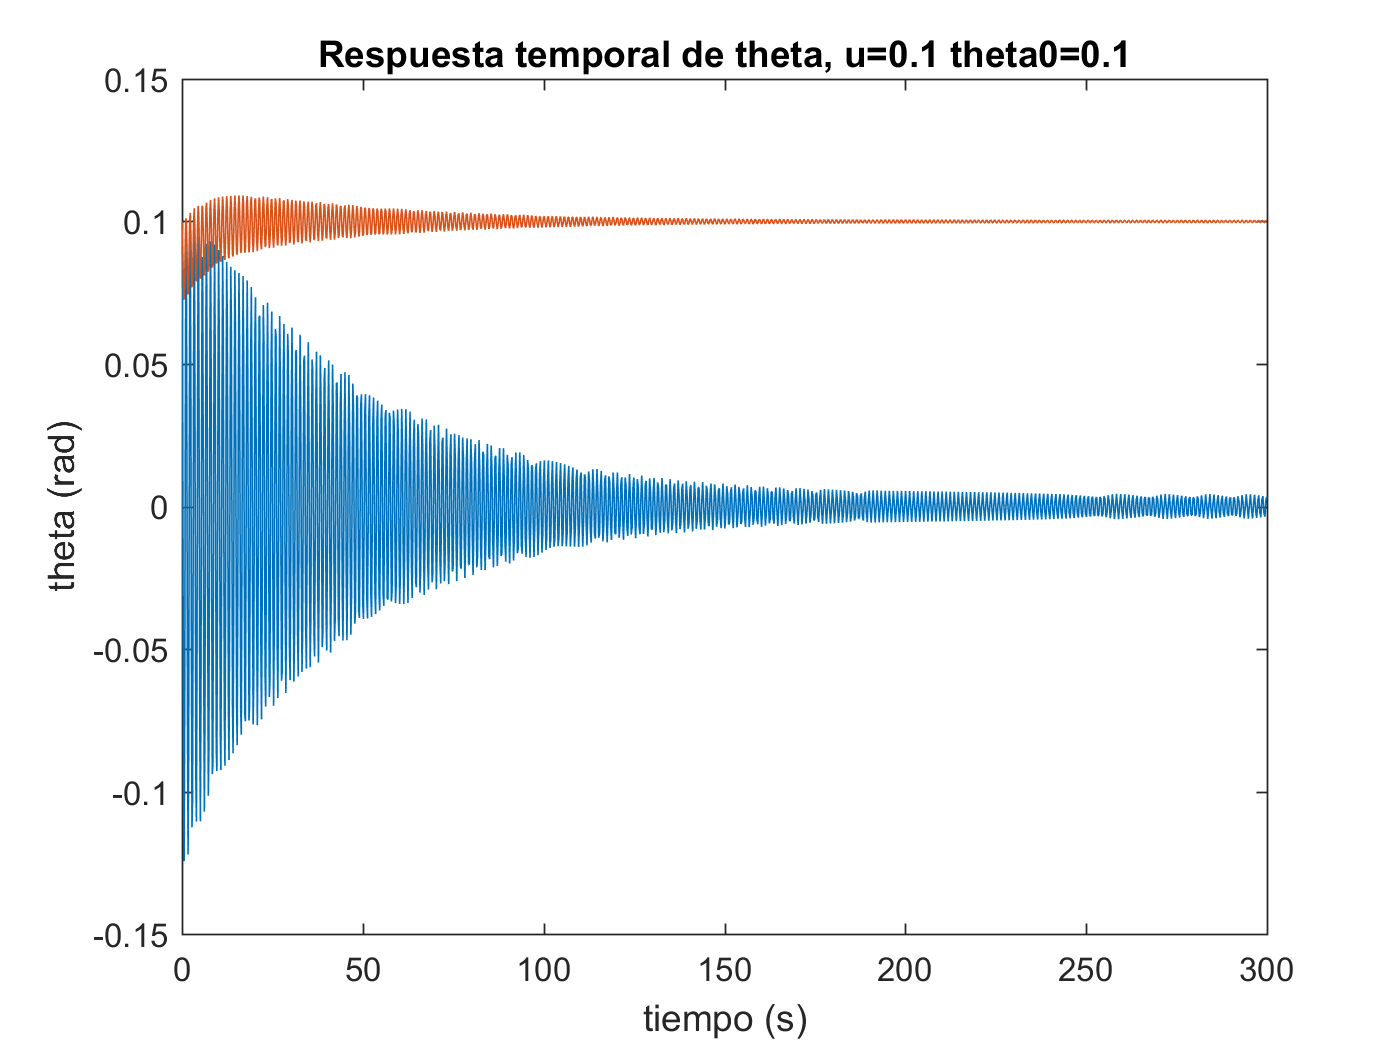
\includegraphics[scale=0.19]{Graficaslvsnl/t0_1.png}
\end{figure}

\section{Función de transferencia}
La función de transferencia es un modelo matemático que relaciona la respuesta de un sistema con una señal de entrada por medio de un cociente. Para un sistema en tiempo continuo, viene a ser la transformada de Laplace de la salida sobre la transformada de Laplace de la entrada, bajo la suposición de condiciones iniciales nulas \cite{wiki:state} . Mientras que, para uno en tiempo discreto, se realiza el mismo procedimiento que en tiempo continuo pero con la transformada Z.   

\subsection{Función de transferencia continua}\label{sub:ftc}
El péndulo invertido es un sistema SIMO, es decir, posee una sola entrada y múltiples salidas. Por lo cual, se habla de una matriz de transferencia, donde se tiene un función de transferencia por cada par entrada-salida. La matriz de transferencia se muestra en (\ref{tf: G}). La función de transferencia correspondiente al par $u-y_1$ se referirá como $G_1$ y al par $u-y_2$ como $G_2$.

\begin{equation}
\label{tf: G}
 G(s) = \begin{bmatrix}
	y_1(s)\\
	y_2(s)
\end{bmatrix} = 
\begin{bmatrix}
    \dfrac{1.818 s^2 + 44.55}{s^4 + 0.1818 s^3 + 31.18 s^2 + 4.455 s}\\
	\dfrac{-4.545 s}{s^3 + 0.1818 s^2 + 31.18 s + 4.455}
\end{bmatrix}
\begin{bmatrix}
	u(s)
\end{bmatrix}
\end{equation}
\textbf{}

Para cualquier función de transferencia se denomina polos a las raíces del denominador, también conocido como polinomio característico, y ceros a las del numerador. La ganancia es la constante o la``amplitud" de la función, la cual no necesariamente debe ser positiva. Una función de transferencia ($TF$) con numerador de grado $m$ y denominador de grado $n$, se puede expresar en términos de sus polos ($p$), ceros ($z$) y ganancia ($k$) de la siguiente forma
\[
TF(s) = k\dfrac{(s - z_1)...(s - z_m)}{(s - p_1)...(s - p_n)}
\]
Los polos, ceros y ganancia por cada para entrada-salida de la función de transferencia del modelo lineal del péndulo invertido se muestran en el Cuadro \ref{tab: pzg tfc}. La graficación de los polos y ceros de $G$ se encuentran en la Figura \ref{fig:pzG}. Tanto del Cuadro \ref{tab: pzg tfc} como de la Figura \ref{fig:pzG}, se aprecian raíces complejas conjugadas y raíces reales, todas negativas exceptuando un polo en 0. El polo que se encuentra en 0 proviene de $G_1$. Dicho polo hace que el sistema se considere críticamente estable, validando el estudio de la estabilidad del sistema por medio de los valores propios de la matriz A que se encuentra en la Sección \ref{sec:lin}. Si la salida del sistema fuese únicamente el ángulo $\theta$, el sistema sería estable.\\

\begin{table}[!h]
\centering
\caption{Polos, ceros y ganancia de la función de transferencia continua reducida a orden dos}
\label{tab: pzg tfc}
\begin{tabular}{@{}lccc@{}}
\toprule
                  & Polos & Ceros             & Ganancia          \\ \midrule
\multirow{4}{*}{$G_1$} & 0 & 4.9497i & 1.8182 \\
                  & -0.0195 + 5.5835i &        -4.9497i           &                   \\
                  & -0.0195 - 5.5835i & &                   \\
                  &    -0.1429  &                   &                   \\ \midrule
\multirow{3}{*}{$G_2$} & -0.0195 + 5.5835i & 0 & -4.5455 \\
                  & -0.0195 - 5.5835i &           &                   \\
                  & -0.1429 & &                  
                  \\ \bottomrule
\end{tabular}
\end{table}


\begin{figure}[ht!]
\caption{Mapa de polos y ceros de $G$\label{fig:pzG}}
  \centering
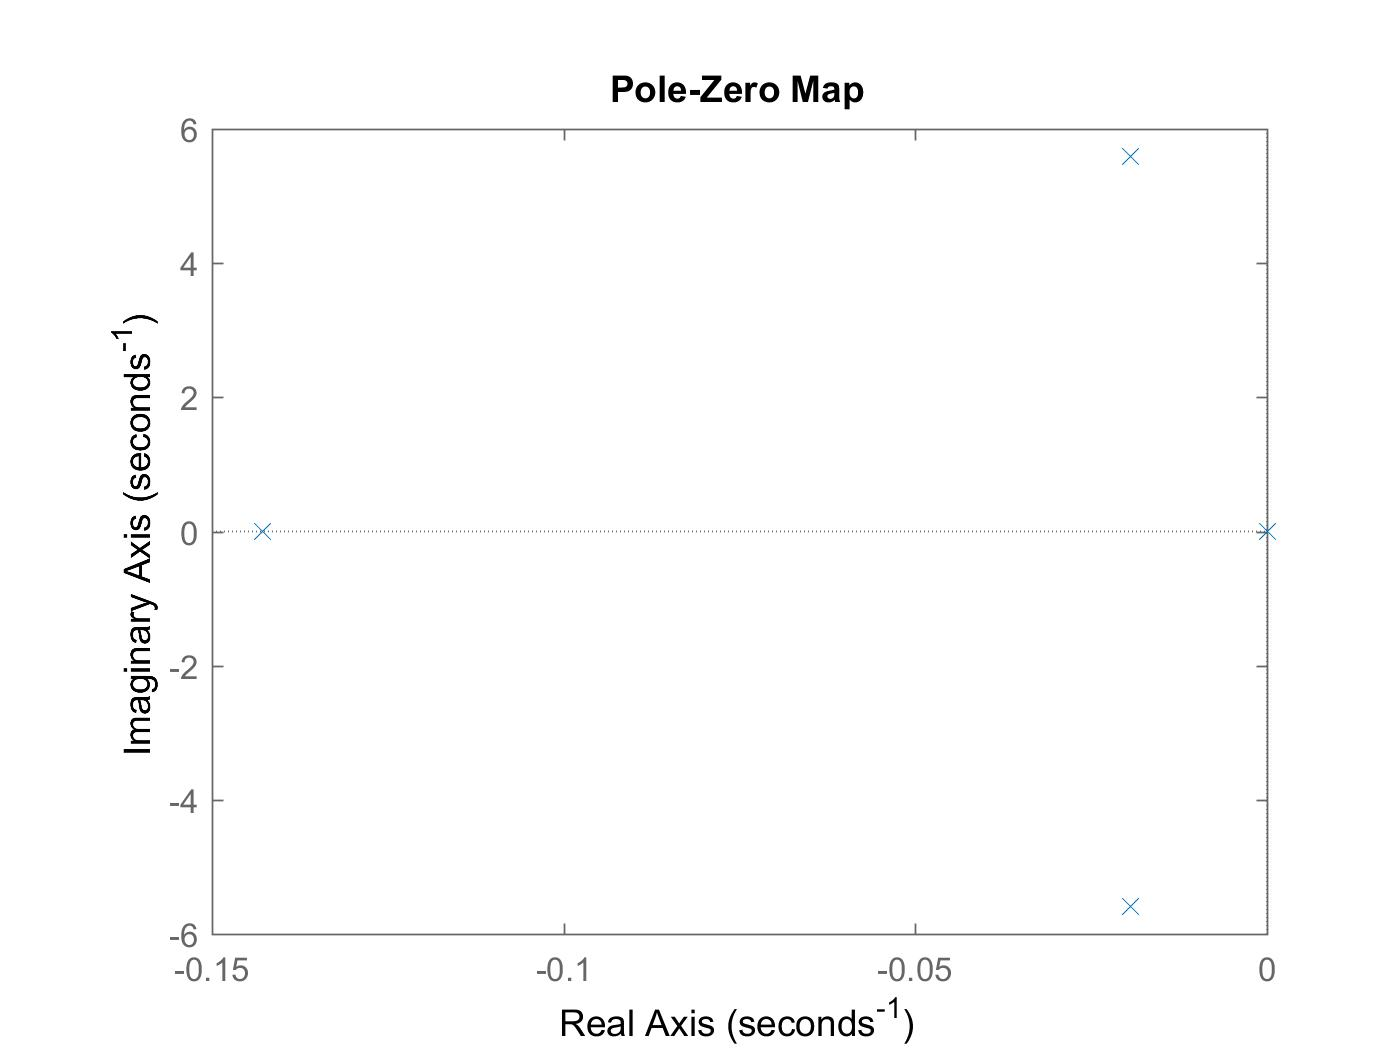
\includegraphics[scale=0.18]{tf/pzmap_G.jpg}
\end{figure}

\subsubsection*{Respuesta al escalón y al impulso unitario}
Al sistema se le aplican dos tipos de entrada: escalón e impulso, ambas unitarias. Las respuestas temporales para el escalón unitario se muestran en la Figura \ref{fig:step}. Al contrastar las Figuras \ref{x1step} y \ref{x3step} con la Figura \ref{fig:step}, se encuentra que ambas respuestas coinciden. La comparación se hace a partir del momento de acción de la entrada, por lo que se deben despreciar los primeros 5 segundos en las gráficas del escalón retardado. Por otro lado, las respuestas al impulso unitario se encuentran en la Figura \ref{fig:impulse}. La variable $x_1$ explota al aplicar el escalón, mas converge a un valor al aplicar el impulso. Una explicación factible es que el escalón unitario se ve como una fuerza positiva constantemente entrando al sistema haciendo que la posición tenga un crecimiento positivo permanente. La variable $x_3$ tiene un comportamiento más similar para ambas señales, convergiendo a 0.\\      
\begin{figure}[ht!]
\caption{Respuesta temporal de las salidas a la entrada escalón unitario\label{fig:step}}
  \centering
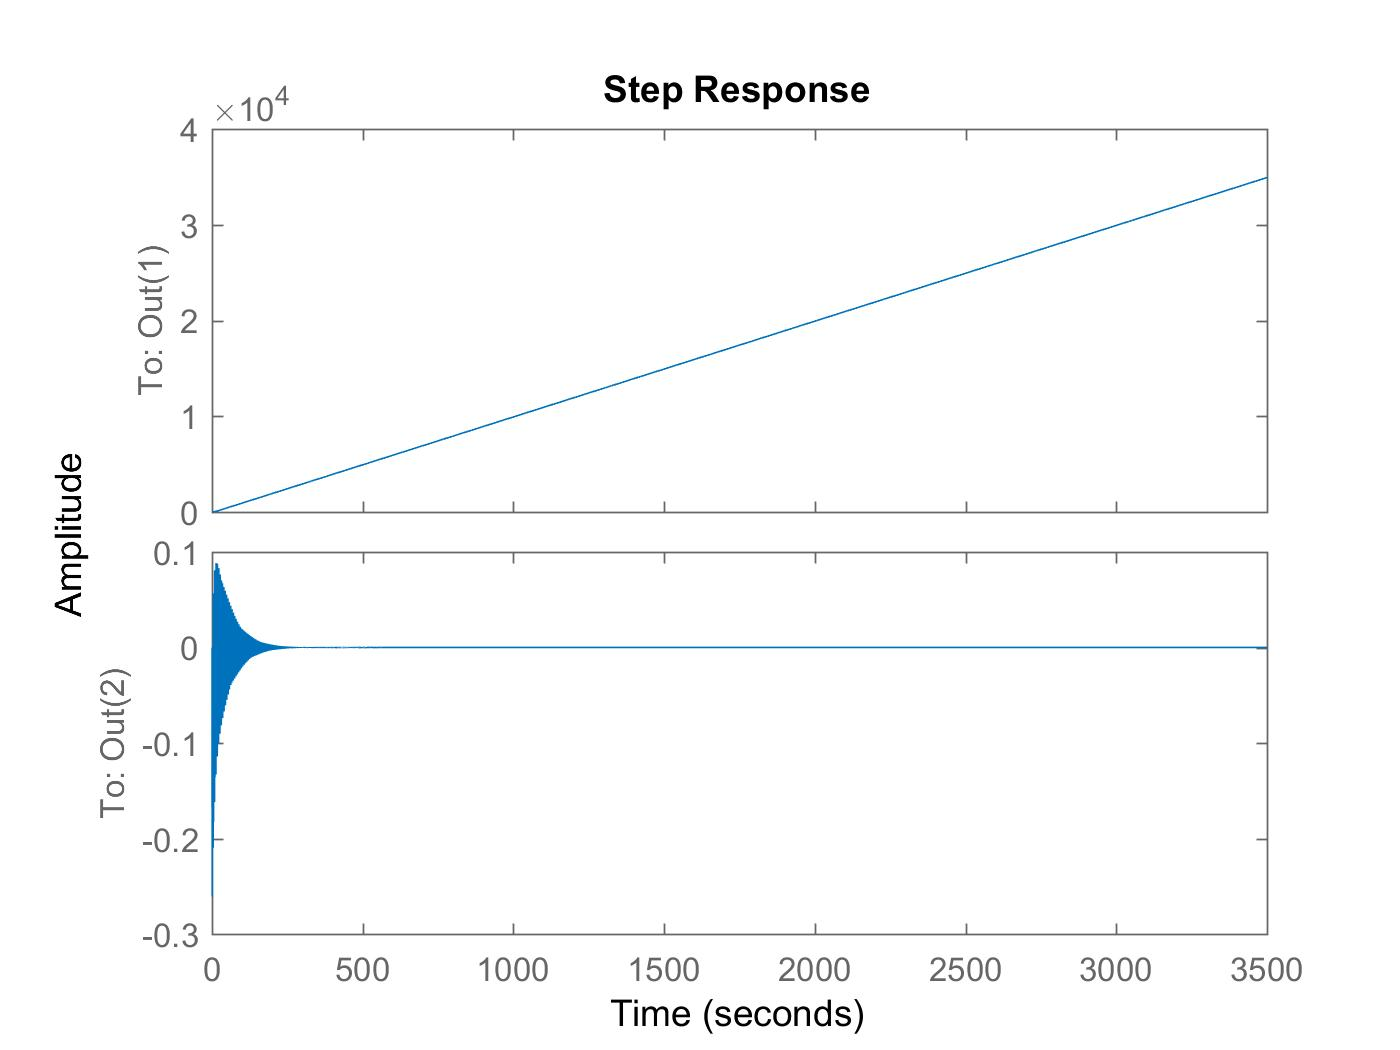
\includegraphics[scale=0.18]{tf/step.jpg}
\end{figure}

\begin{figure}[ht!]
\caption{Respuesta temporal de las salidas a la entrada impulso unitario\label{fig:impulse}}
  \centering
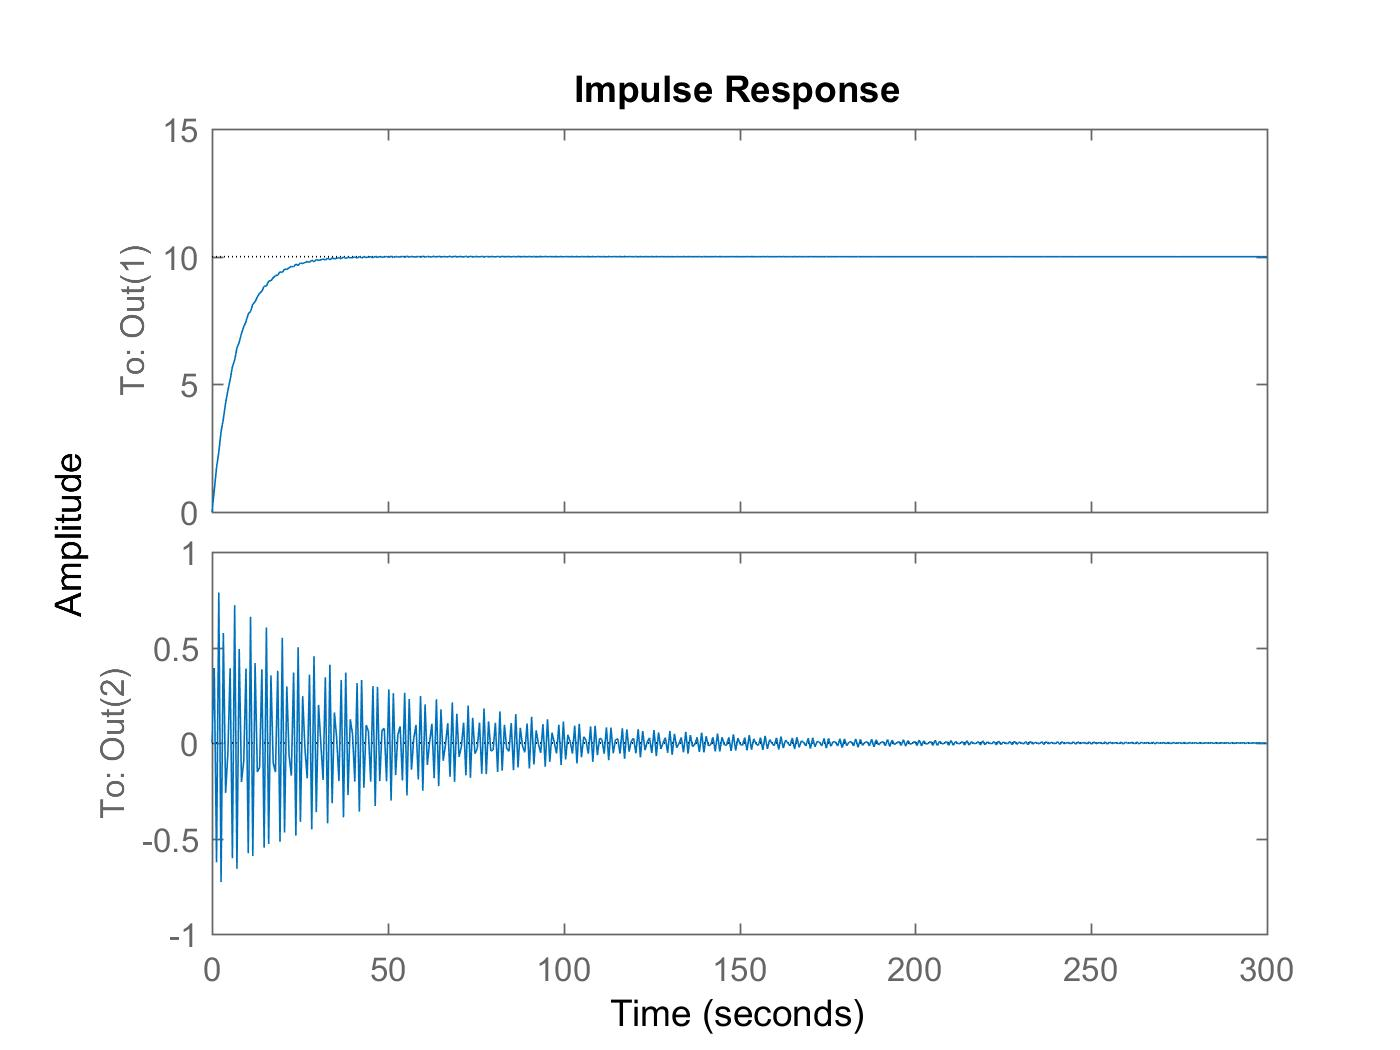
\includegraphics[scale=0.18]{tf/impulse.jpg}
\end{figure}

\subsubsection*{Estado estacionario}
El teorema del valor final se utiliza cuando es necesario determinar el comportamiento de la función $y(t)$ en el infinito. Para cada función de transferencia $G_1$ y $G_2$, se evalúa la salida en estado estacionario aplicando el teorema del valor final
\[
\lim_{s \to 0} sG(s)
\]
Los resultados obtenidos de la evaluación son $\infty$ y 0 para $G_1$ y $G_2$, respectivamente. Esto quiere decir que la salida $y_1$ diverge; mientras que, la salida $y_2$ converge a 0, es decir, posee estado estacionario. 

\subsection{Reducción de la función de transferencia continua a segundo orden}
La función de transferencia del modelo, presentada en la Subsección \ref{sub:ftc}, es de cuarto orden. El orden de una función de transferencia se identifica por el orden de su denominador. La idea es reducirla a una de segundo orden y compararlas. Esta reducción se lleva a cabo por medio del comando de MATLAB \textit{reduce}. La matriz de transferencia resultante se muestra a en (\ref{tf:Gr}).\\ 

\begin{equation}
\label{tf:Gr}
Gr(s)=\begin{bmatrix}
	y_1(s)\\
	y_2(s)
\end{bmatrix} = 
\begin{bmatrix}
\dfrac{0.00468 s + 1.428}{s^2 + 0.1428 s}\\
\dfrac{-0.0249}{s + 0.1428}
\end{bmatrix}
\begin{bmatrix}
	u(s)
\end{bmatrix}
\end{equation}

Los polos, ceros y ganancia para la función de transferencia por cada par entrada-salida se presentan en el Cuadro \ref{tab: pzg tfr} y el gráfico de polos y ceros del sistema en general ($Gr$) en la Figura \ref{fig:pzGr}. La Figura \ref{fig:pzGr} se valida al mirar los valores de los polos presentados en el Cuadro \ref{tab: pzg tfr}. El carácter del sistema en términos de estabilidad se conserva al momento de realizar la reducción, sigue siendo críticamente estable. Los polos negativos complejos conjugados desaparecen y se conservan el que se encuentra en 0 y el real negativo en la función de transferencia reducida.

\begin{table}[!h]
\centering
\caption{Polos, ceros y ganancia de la función de transferencia continua}
\label{tab: pzg tfr}
\begin{tabular}{@{}lccc@{}}
\toprule
                  & Polos & Ceros             & Ganancia          \\ \midrule
\multirow{2}{*}{$Gr_1$} & -0.1428 & -305.0361 & 0.0047 \\
                  & -0 & &                   \\
                 \midrule
$Gr_2$ & -0.1428 &  & -0.0249                 
                  \\ \bottomrule
\end{tabular}
\end{table}

\begin{figure}[ht!]
\caption{Mapa de polos y ceros de $Gr$\label{fig:pzGr}}
  \centering
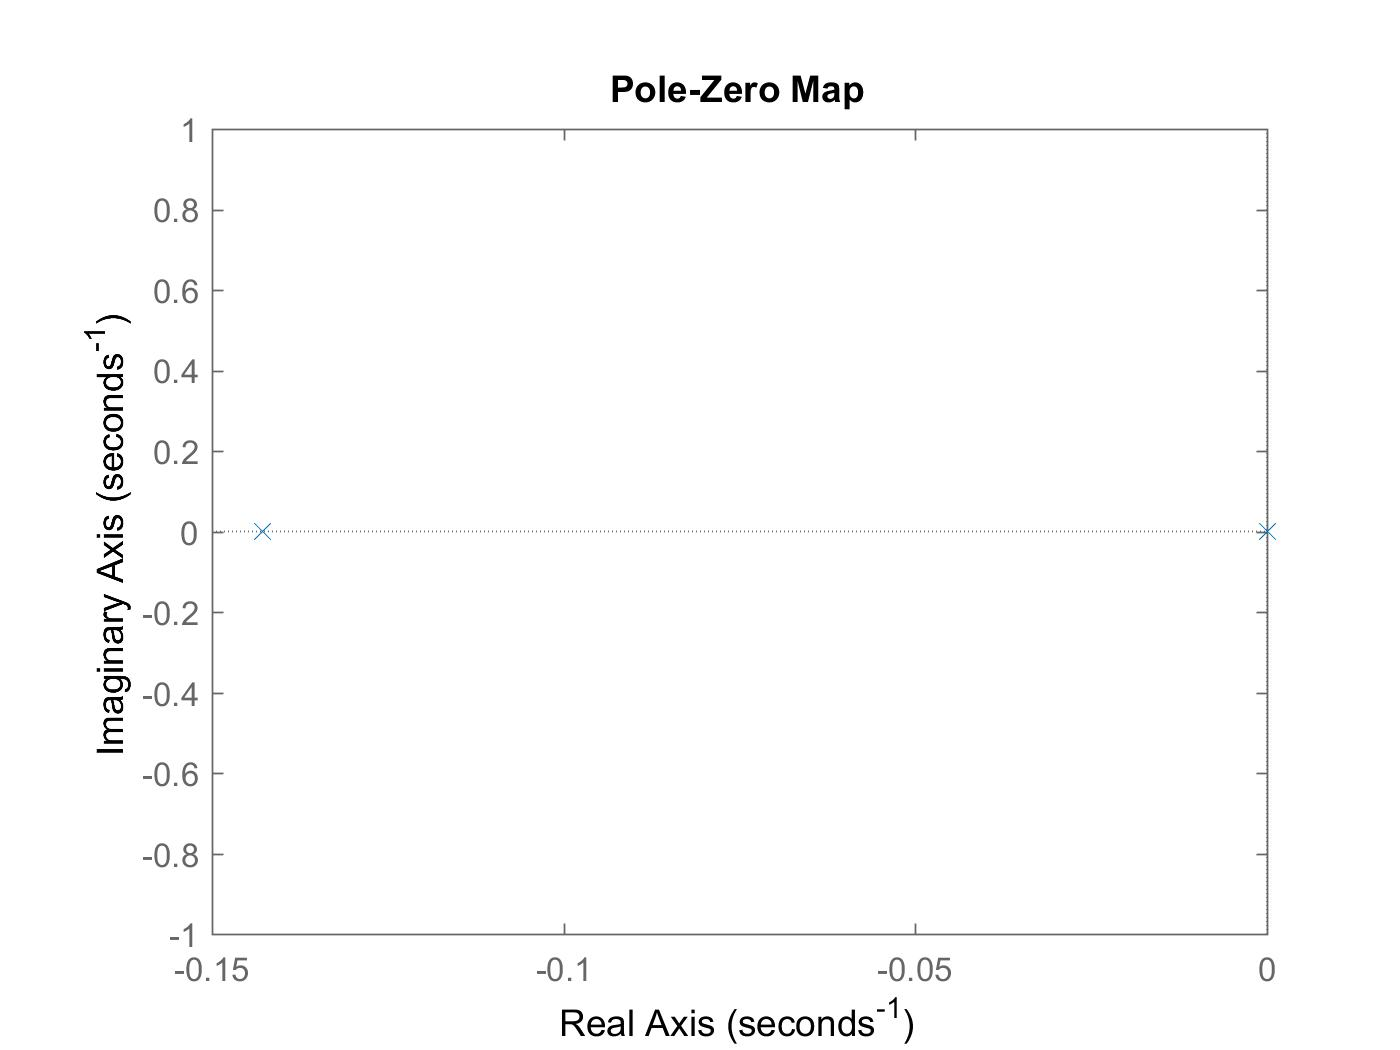
\includegraphics[scale=0.18]{tf/pzmap_Gr.jpg}
\end{figure}

\subsubsection*{Respuesta al escalón y al impulso unitario}
Las respuestas al escalón y al impulso unitarios del sistema reducido se ven en las Figuras \ref{fig:stepGr} y \ref{fig:impulseGr}. Para la salida $y_1$ se ve un comportamiento igual al observado para el sistema con orden completo en respuesta a ambas entradas. Aunque esto no se puede decir para $y_2$. La respuesta temporal para ambas entradas no presenta oscilación, como sí ocurre con las de la función de transferencia de orden completo. Para el impulso unitario, la salida también converge a 0, como ocurre en la subsección anterior, y el punto de corte con el eje de ordenadas ($-0.025$) hace parte del rango de oscilación de la respuesta original ([$-0.7;0.7$]). La respuesta al escalón unitario es más especial, ésta no converge 0, sino a $-0.174$, difiriendo con la original. 

\begin{figure}[ht!]
\caption{Respuesta temporal de las salidas a la entrada escalón unitario\label{fig:stepGr}}
  \centering
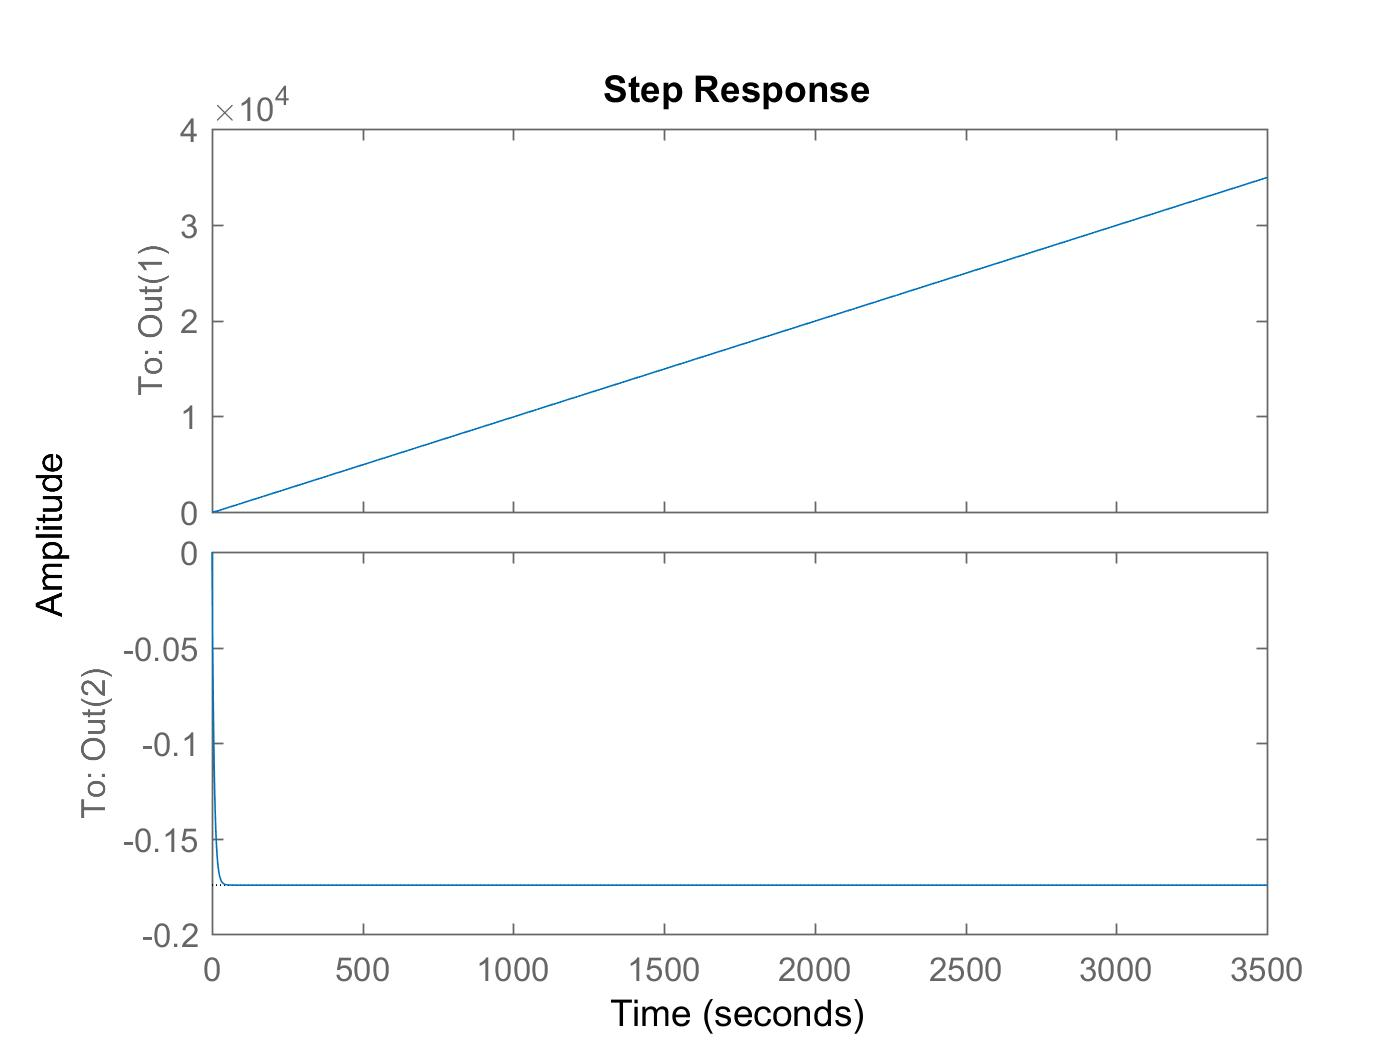
\includegraphics[scale=0.18]{tf/step_Gr.jpg}
\end{figure}

\begin{figure}[ht!]
\caption{Respuesta temporal de las salidas a la entrada impulso unitario\label{fig:impulseGr}}
  \centering
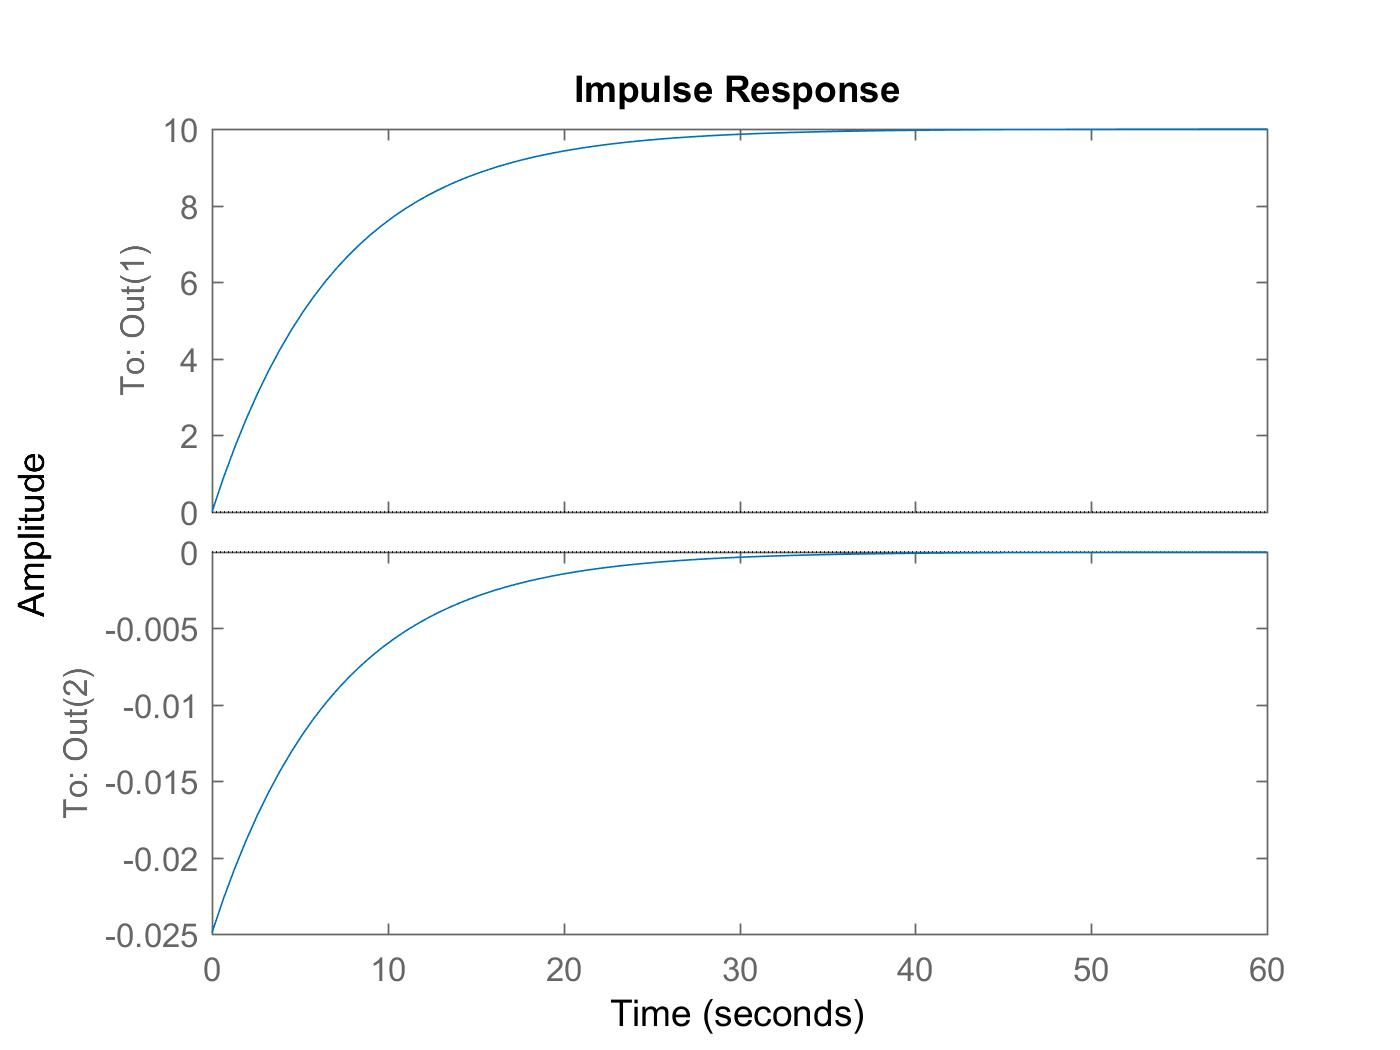
\includegraphics[scale=0.18]{tf/impulse_Gr.jpg}
\end{figure}

\subsection{Función de transferencia discreta}
La función de transferencia continua fue discretizada en tres tiempos de muestreo: $0.21$, $0.73$ y $1.26$. Se presentan los mapas de polos y ceros para las tres discretizaciones obtenidas, junto con las respuestas temporales a las entradas escalón unitario e impulso unitario, en las Figuras \ref{fig:pzGd}-\ref{fig:impulseGd2}. Los mapas de polos y ceros para la función discretizada en los diferentes tiempos de muestreo tienen en común un polo en la frontera del círculo unitario, específicamente en ($1,0$). A medida que se aumenta el tiempo de muestreo, los polos aumentan su distancia al círculo unitario. El sistema en ninguna de las discretizaciones pierde su carácter de críticamente inestable. De forma similar ocurre con las respuestas temporales al impulso unitario, en las cuales se halla un gran parecido con las respuestas temporales a la misma entrada de la función de transferencia continua. A medida que se aumenta el tiempo de muestreo, se percibe un deterioro en curvas, especialmente en la de la salida $y_1$ antes de converger con la aparición de un despicado y en la de la salida $y_2$ donde las distancia entre las oscilaciones es cada vez mayor y éstas son más toscas.\\ 

\begin{figure}[h!]
\caption{Mapa de polos y ceros para la función de transferencia con $T=0.21$\label{fig:pzGd}}
  \centering
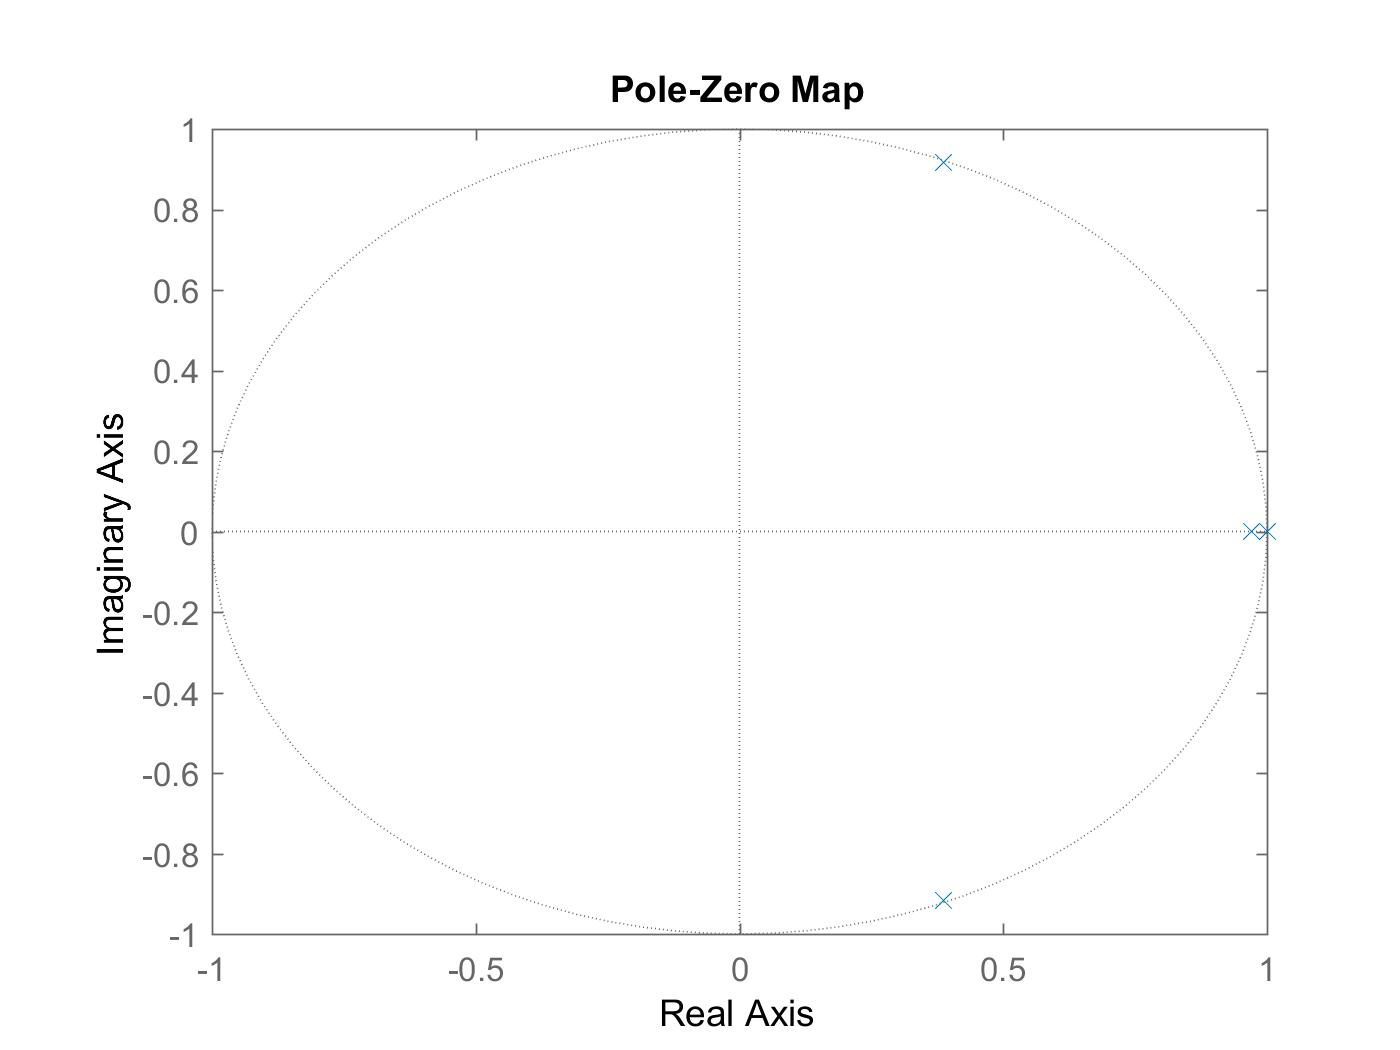
\includegraphics[scale=0.18]{tf/pzmap_Gd.jpg}
\end{figure}

\begin{figure}[h!]
\caption{Mapa de polos y ceros para la función de transferencia con $T=0.73$\label{fig:pzGd1}}
  \centering
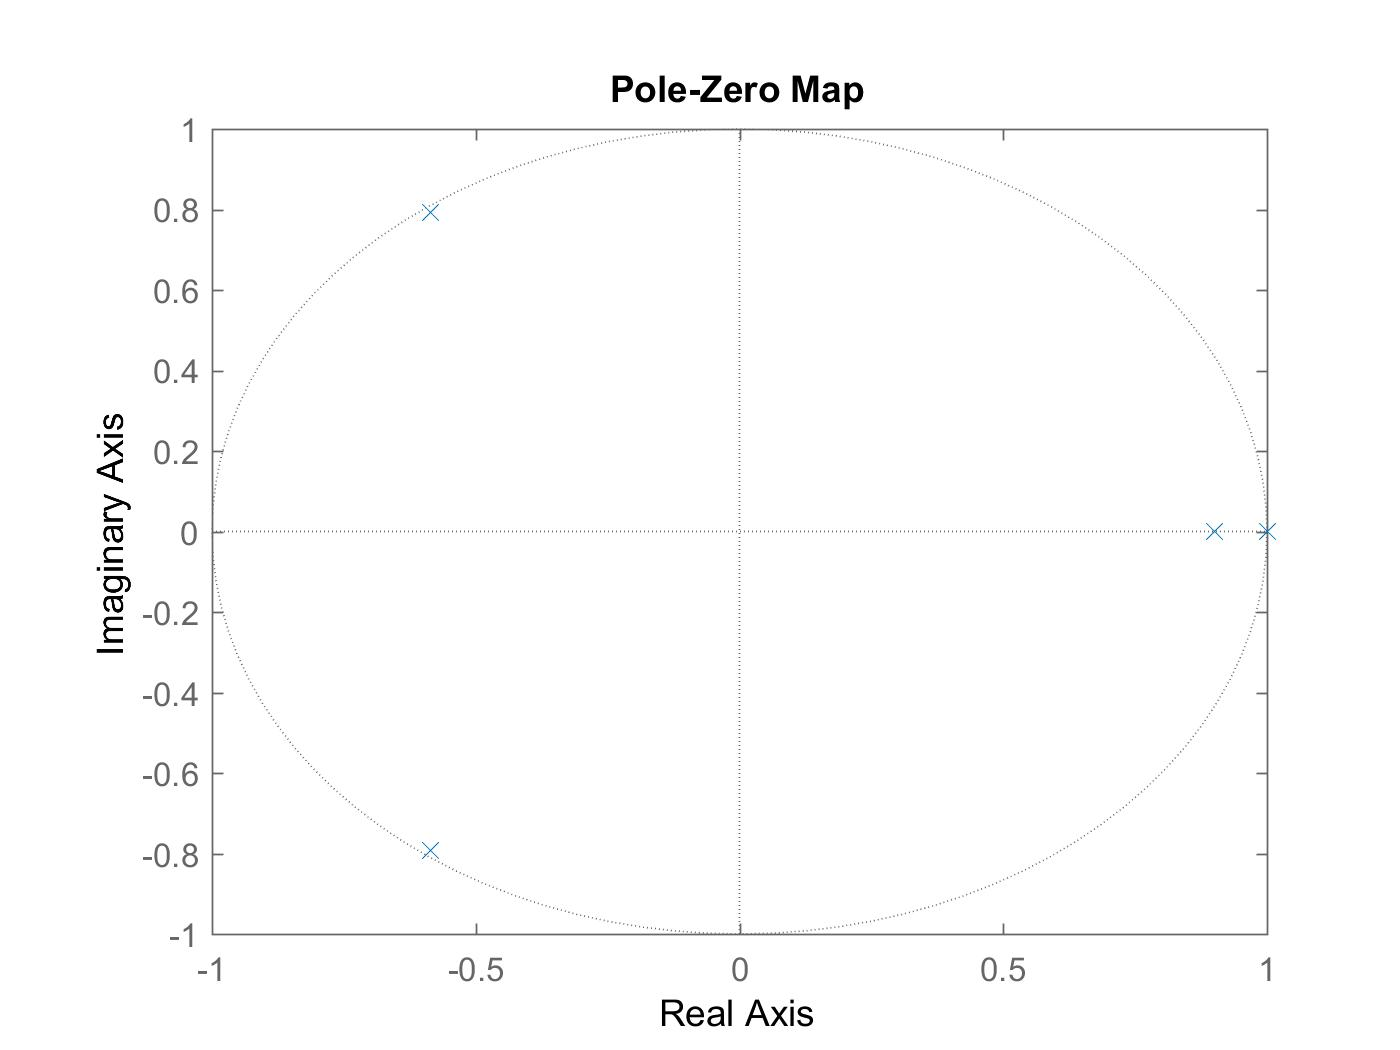
\includegraphics[scale=0.18]{tf/pzmap_Gd_1.jpg}
\end{figure}

\begin{figure}[h!]
\caption{Mapa de polos y ceros para la función de transferencia con $T=1.26$\label{fig:pzGd2}}
  \centering
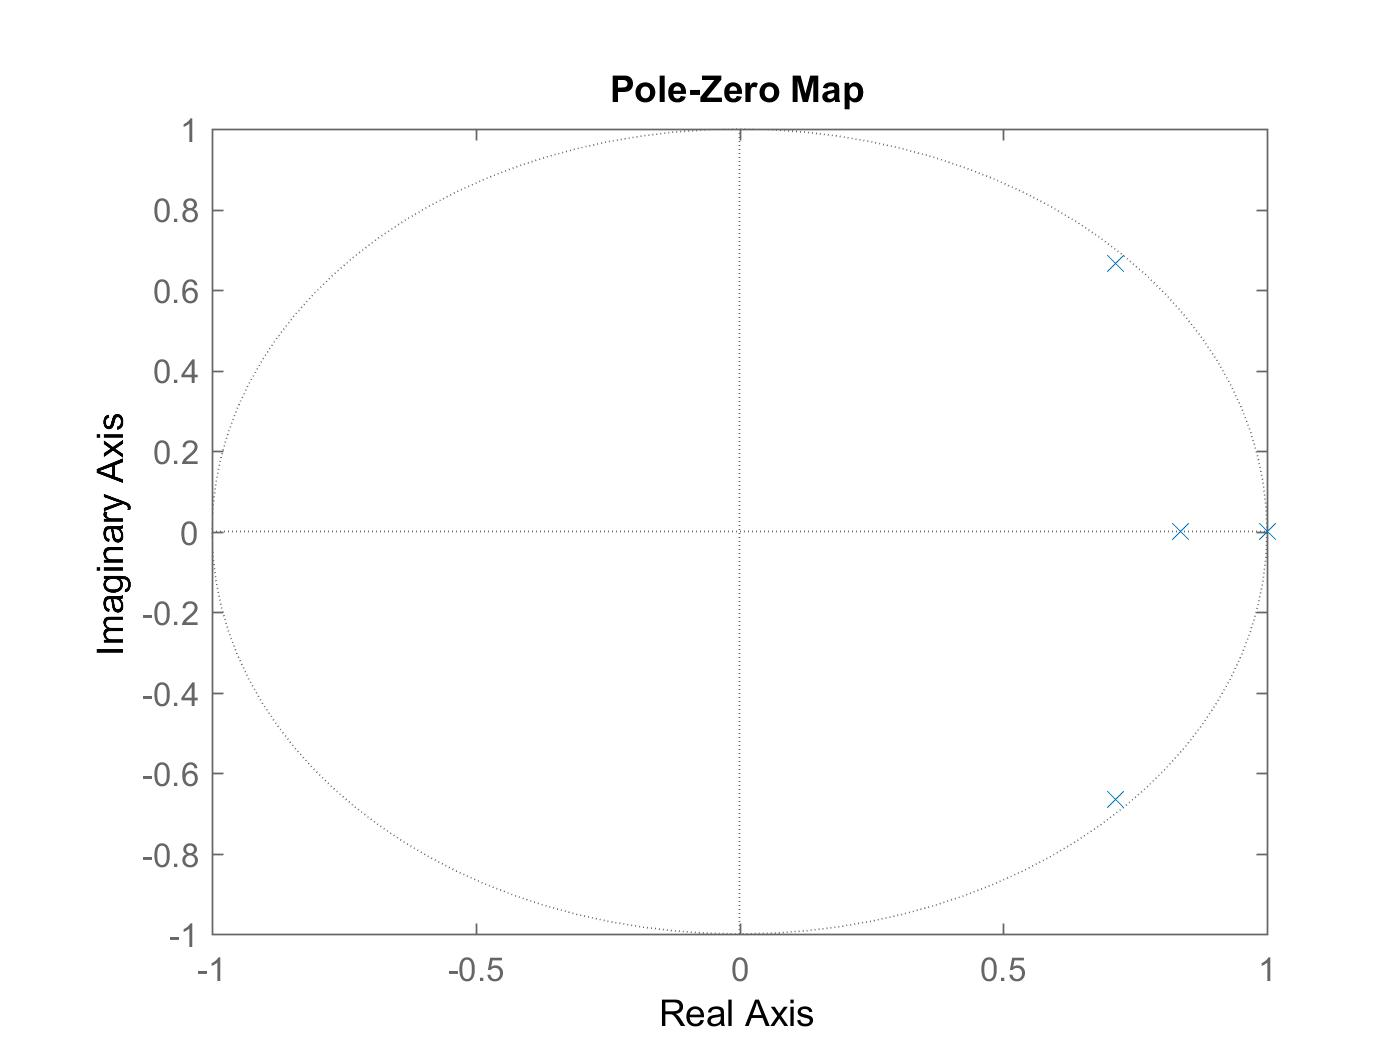
\includegraphics[scale=0.18]{tf/pzmap_Gd_2.jpg}
\end{figure}

\begin{figure}[h!]
\caption{Respuesta temporal de las salidas a la entrada impulso unitario para la f. de transferencia de $T=0.21$\label{fig:impulseGd}}
  \centering
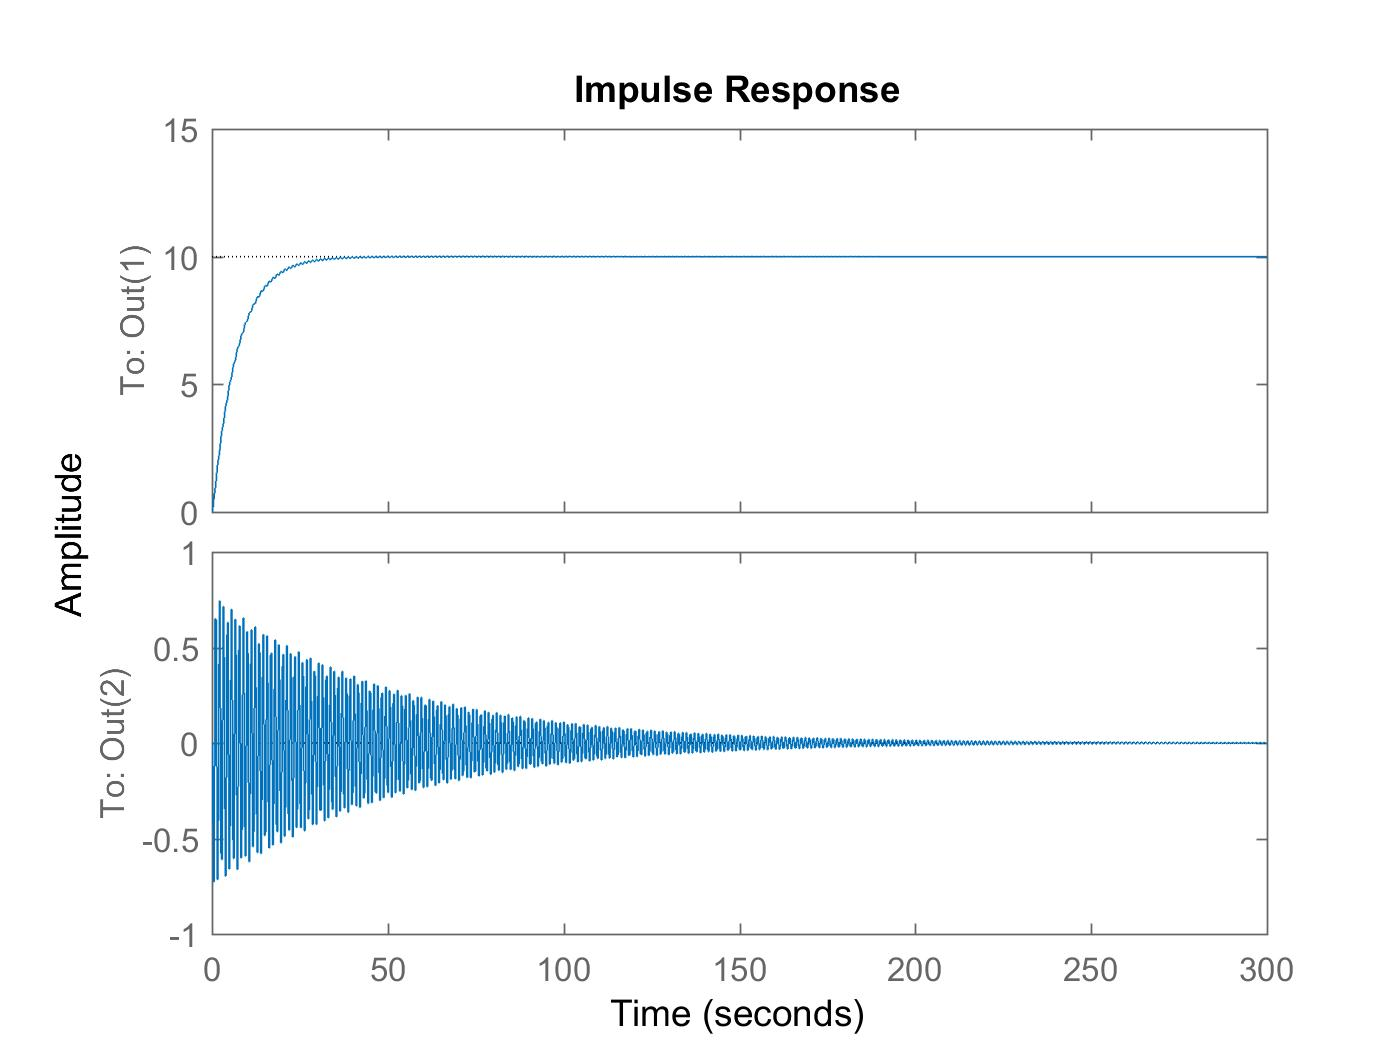
\includegraphics[scale=0.18]{tf/impulse_Gd.jpg}
\end{figure}

\begin{figure}[h!]
\caption{Respuesta temporal de las salidas a la entrada impulso unitario para la f. de transferencia de $T=0.73$\label{fig:impulseGd1}}
  \centering
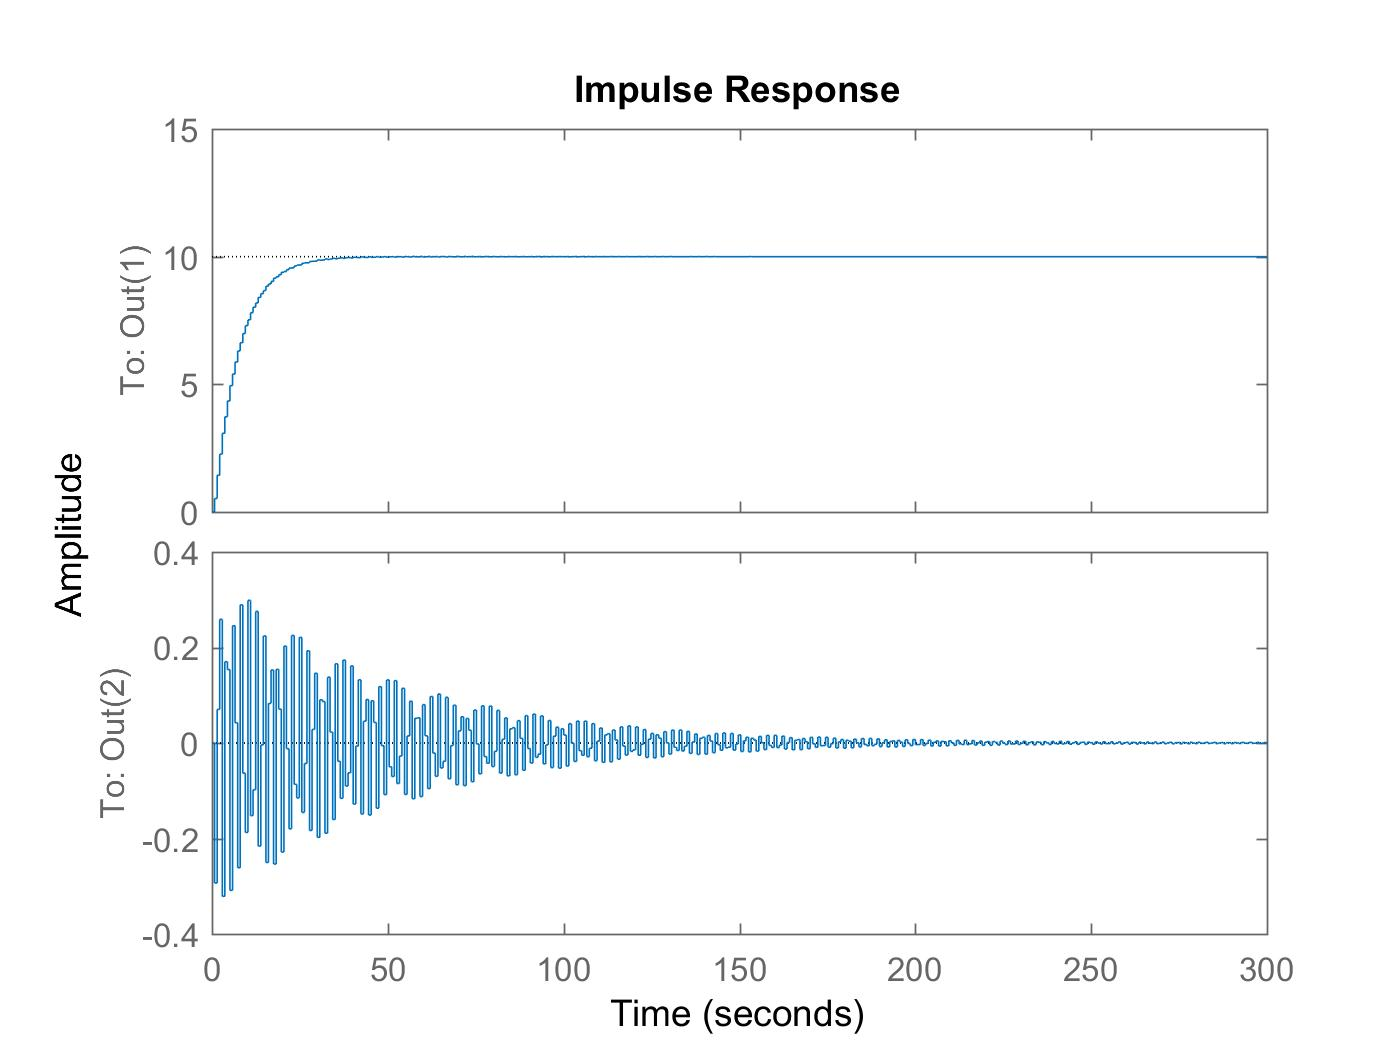
\includegraphics[scale=0.18]{tf/impulse_Gd_1.jpg}
\end{figure}

\begin{figure}[h!]
\caption{Respuesta temporal de las salidas a la entrada impulso unitario para la f. de transferencia de $T=1.26$\label{fig:impulseGd2}}
  \centering
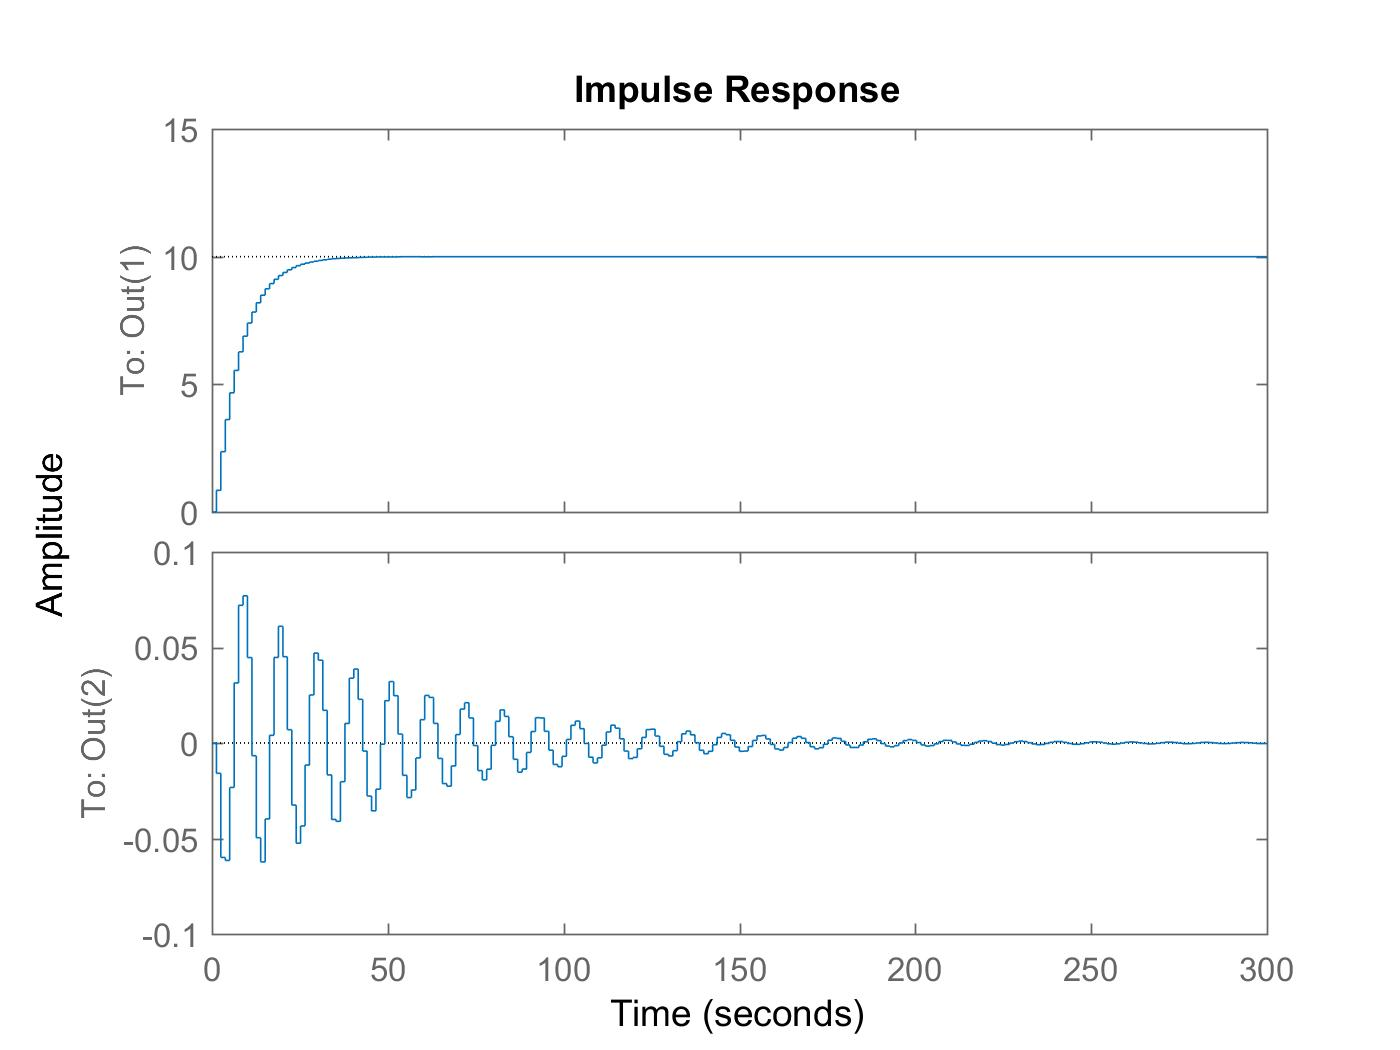
\includegraphics[scale=0.18]{tf/impulse_Gd_2.jpg}
\end{figure}

La función de transferencia discreta que más se asemeja a la función de transferencia continua es la de menor tiempo de muestro ($T=0.21$). Dicha función es la que se presenta detalladamente, en la parte inferior, y en la cual se basan la descripción de polos, ceros y ganancia y la respuesta al escalón unitario.\\

\begin{equation}
\label{tf:Gd}
\begin{aligned}
&Gd(z) = \begin{bmatrix}
	y_1(z)\\
	y_2(z)
\end{bmatrix} \\
& = 
\begin{bmatrix}
\dfrac{0.03866 z^3 - 0.001061 z^2 - 6.895e^{-5} z + 0.03817}{z^4 - 2.743 z^3 + 3.484 z^2 - 2.704 z + 0.9625}\\
\dfrac{-0.08809 z^2 + 0.001042 z + 0.08705}{z^3 - 1.743 z^2 + 1.741 z - 0.9625}
\end{bmatrix}
\begin{bmatrix}
	u(z)
\end{bmatrix}
\end{aligned}
\end{equation}
\textbf{}

Los polos, ceros y ganancia de la función de transferencia (\ref{tf:Gd}) se resumen en el Cuadro \ref{tab: pzg tfd}. Se puede verificar lo anteriormente dicho sobre la estabilidad del sistema: es críticamente estable porque posee un polo en el círculo unitario y el resto de ellos se encuentran al interior de éste. Si la salida únicamente estuviese conformada por $x_3$, el sistema sería estable. Gráficamente lo mencionado se observa en la convergencia de la respuesta temporal de esta salida en las Figuras \ref{fig:impulseGd} y \ref{fig:stepGd}. La respuesta al escalón unitario es idéntica y muy similar a la del caso continuo para $y_1$ y $y_2$, respectivamente.\\

\begin{table}[!h]
\centering
\caption{Polos, ceros y ganancia de la función de transferencia discreta}
\label{tab: pzg tfd}
\begin{tabular}{@{}lccc@{}}
\toprule
                  & Polos & Ceros             & Ganancia          \\ \midrule
\multirow{4}{*}{$Gd_1$} & 0.3862 + 0.9180i & 0.5074 + 0.8617i & 0.0387 \\
                  & 0.3862 - 0.9180i & 0.5074 - 0.8617i &                   \\
                  & 1 & -0.9872 &                   \\
                  & 0.9704 & &                   \\    
                 \midrule
\multirow{4}{*}{$Gd_2$} & 0.9704 & 1 & -0.0881 \\
                  & 0.3862 + 0.9180i & -0.9882 &                   \\  
                  &  0.3862 - 0.9180i &  &
                  \\ \bottomrule
\end{tabular}
\end{table}

\begin{figure}[!h]
\caption{Respuesta temporal de las salidas a la entrada escalón unitario\label{fig:stepGd}}
  \centering
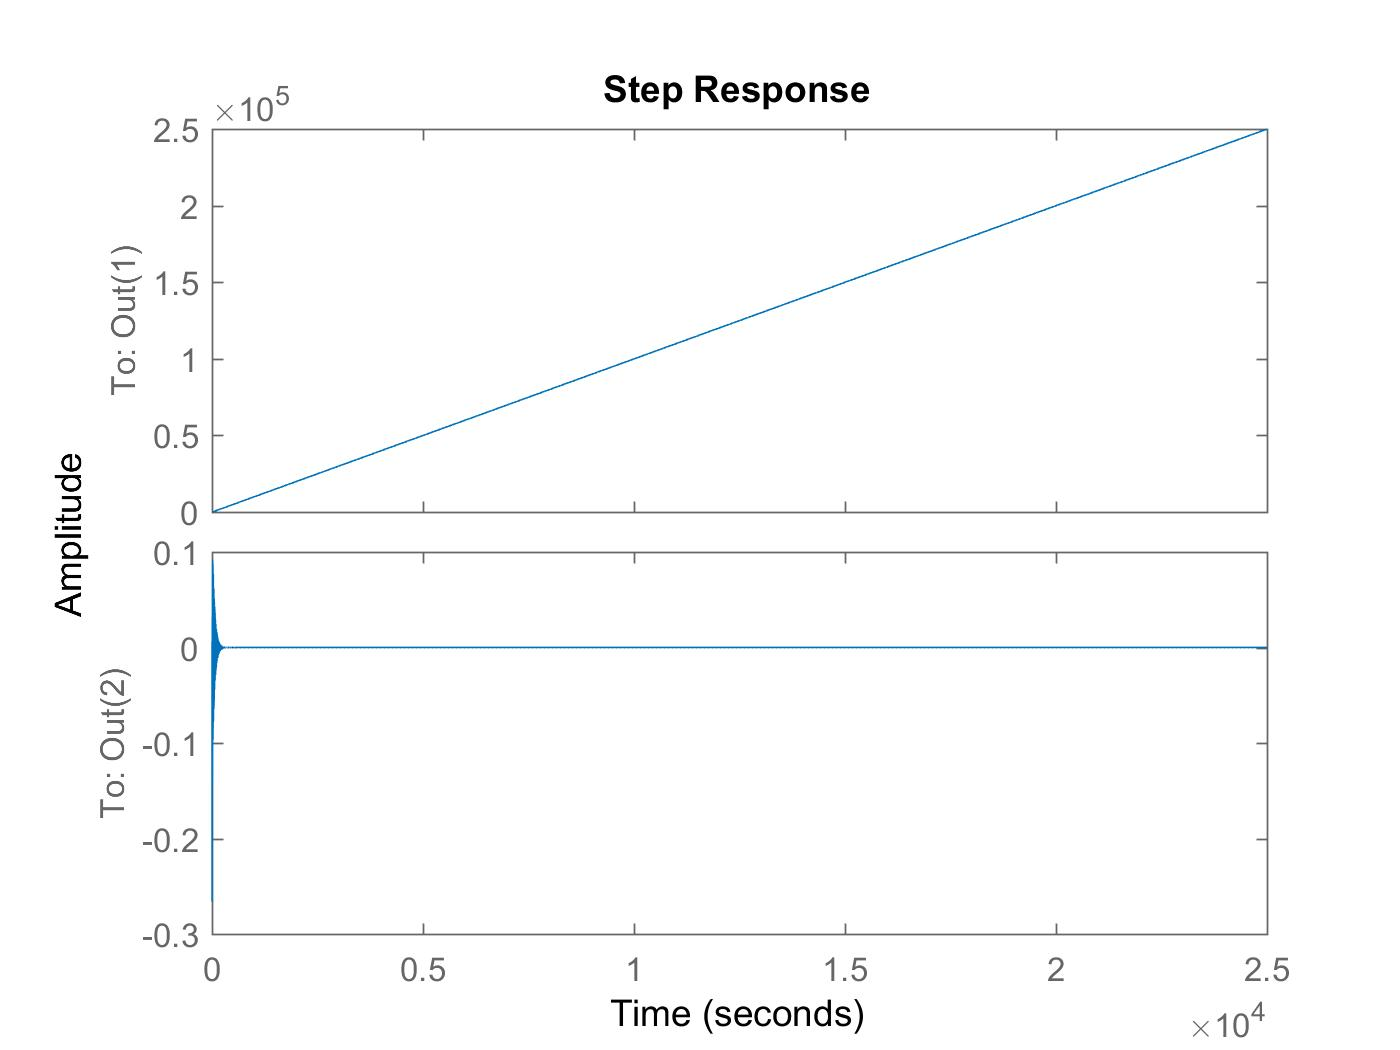
\includegraphics[scale=0.18]{tf/step_Gd.jpg}
\end{figure}

\subsection{Validación de la discretización en \textit{Simulink}}
El entorno de programación visual \textit{Simulink} posee la posibilidad de agregar diferentes tipos de retenedores para discretizar la señal, en la presente subsección se utiliza dicha herramienta con el fin de contrastar y validar los resultados obtenidos, tal como se hizo previamente con el sistema continuo.\\

\begin{figure}[t!]
\caption{Comparación de la discretización realizada en \textit{Simulink} utilizando ZOH y la discretización utilzando \texttt{c2d} de MATLAB, bajo una entrada escalón\label{fig:dis5}}
  %\centering
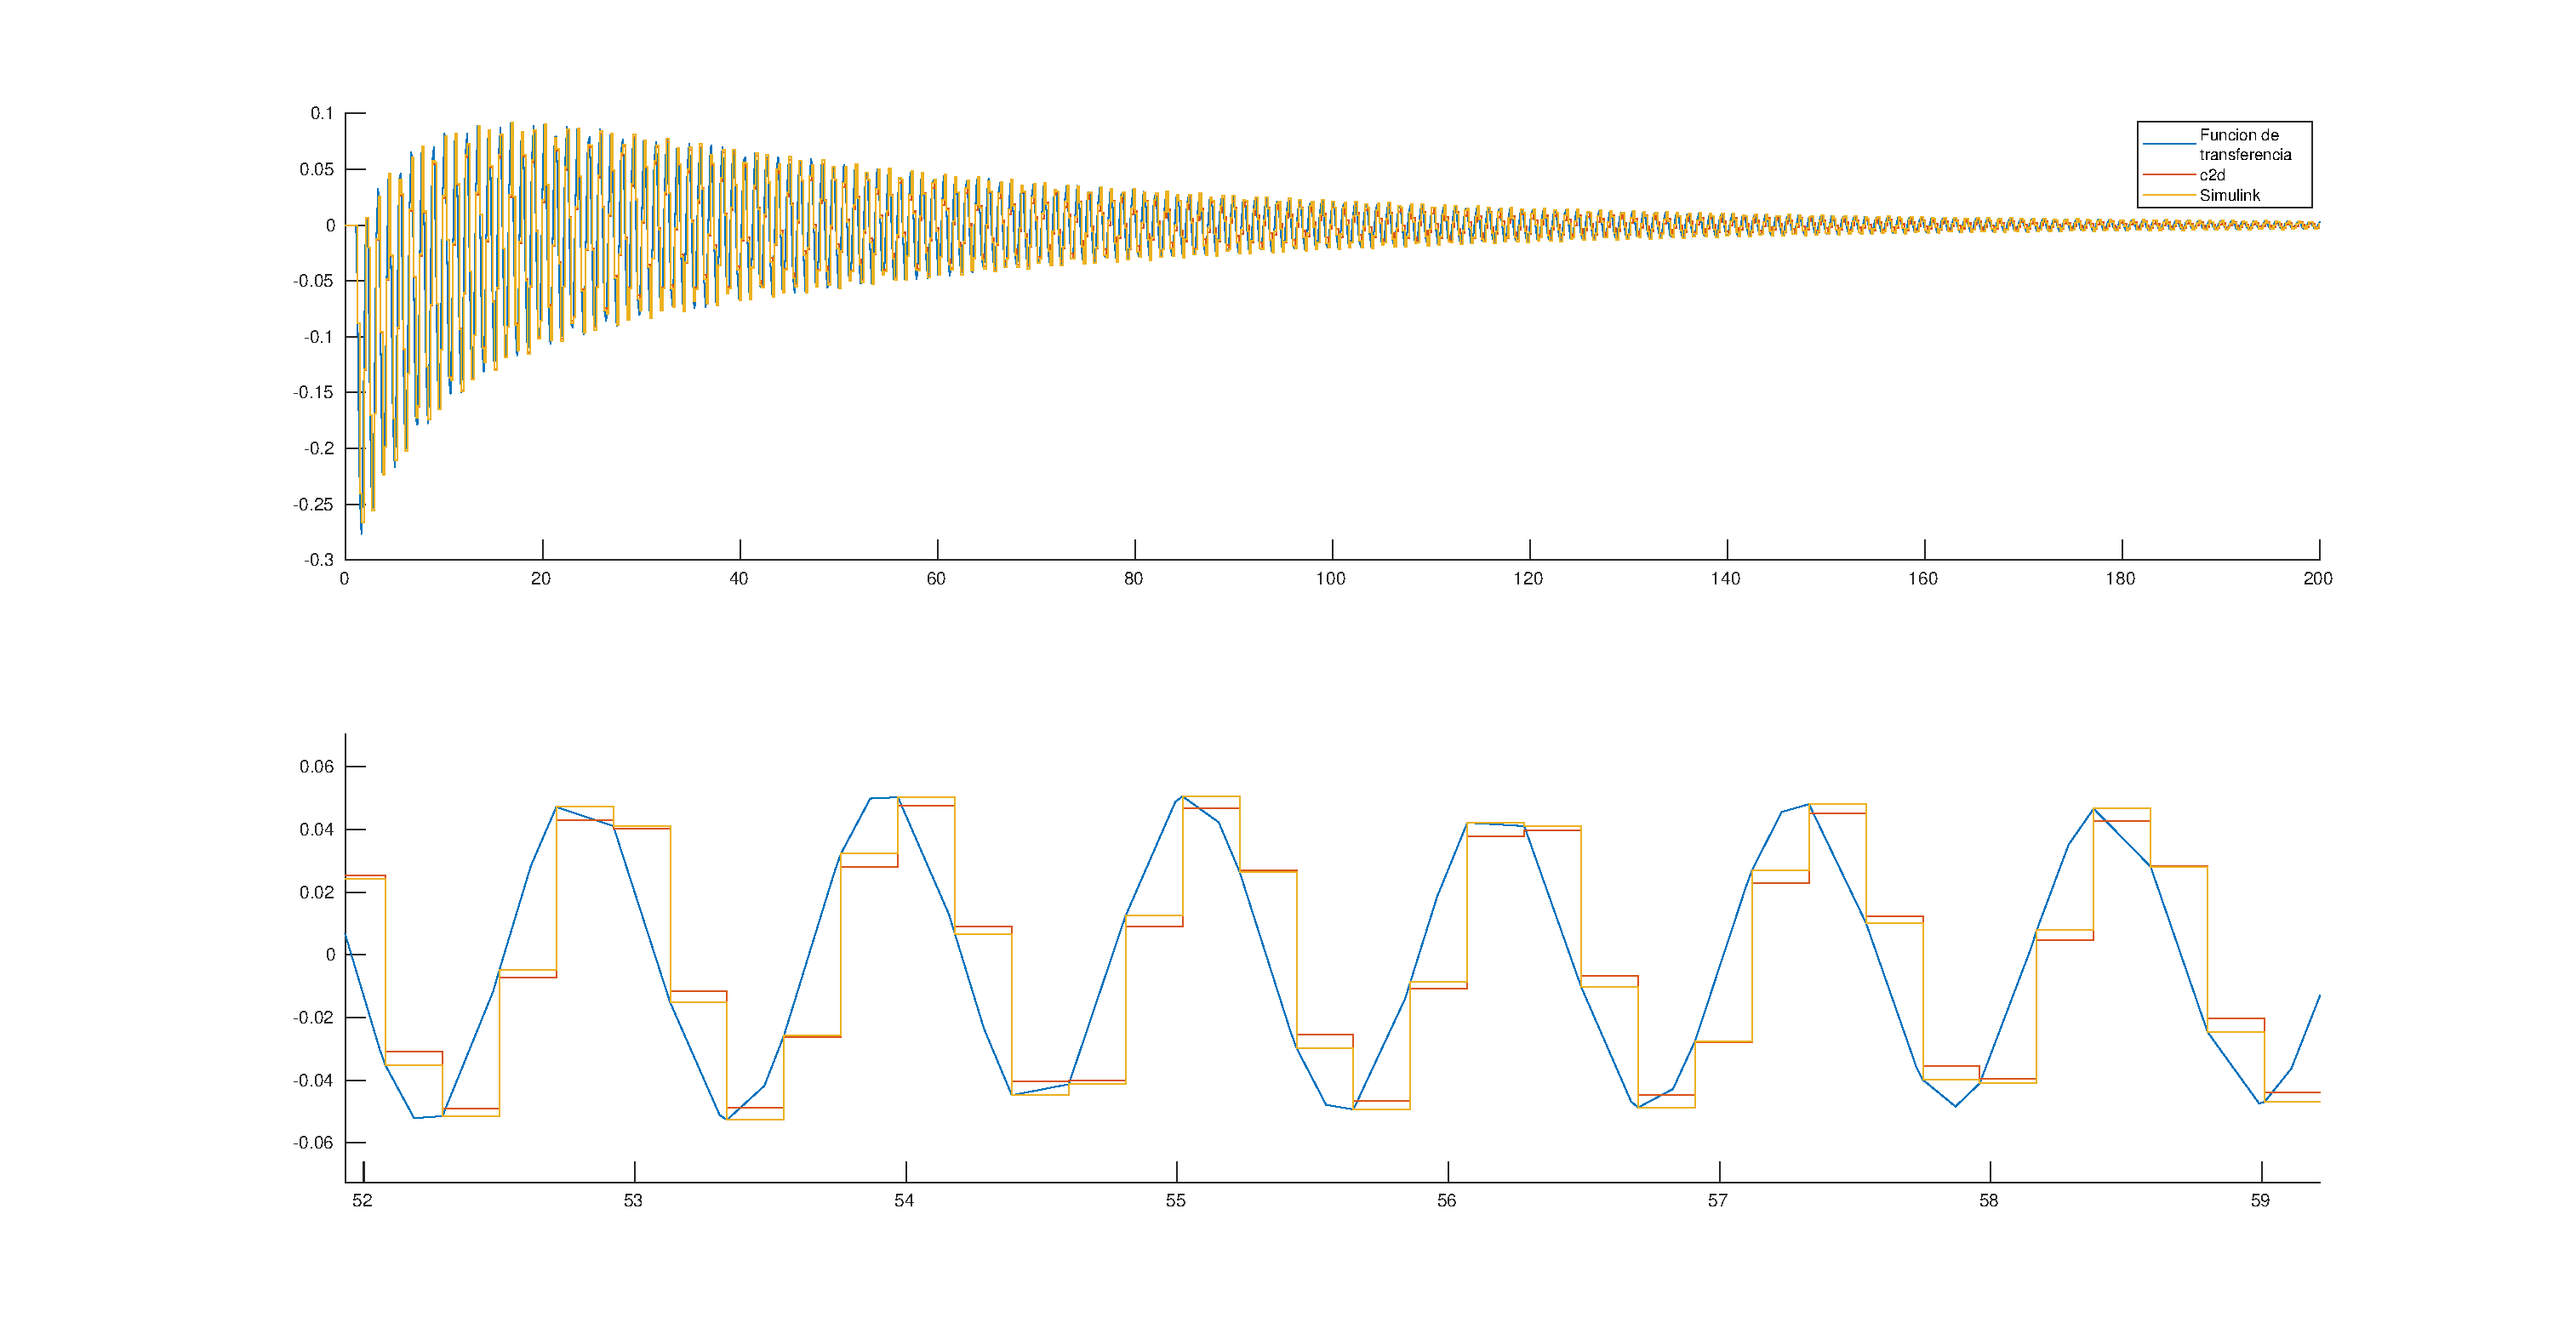
\includegraphics[scale=0.19]{5.eps}
\end{figure}

Con la  finalidad de facilitar el análisis se consideran dos subfiguras. La primera muestra la respuesta temporal para la salida $y_2$ de los diferentes métodos de discretizacion (ZOH y \textit{c2d}) bajo una entrada escalón; sin embargo, por la exactitud de la aproximación es muy difícil comparar las diferentes discretizaciones. Por otro lado, la segunda subfigura muestra un acercamiento a una sección especifica de la primera subfigura, lo que permite observar de manera más clara las diferencias en las señales.\\ 

El primer resultado que se puede deducir al observar la Figura \ref{fig:dis5}, es el hecho de que efectivamente las señales discretas se encuentran sincronizadas, es decir, poseen un mismo periodo de muestreo; sin embargo, también es posible ver éstas difieren un poco. Lo que se puede deber, a que si bien ambas utilizan retenedores de orden cero, ambas están reteniendo señales diferentes, y si bien es un mismo modelo, el modelo de Simulink utiliza un método numérico específico para computar la señal, el cual introduce un error asociado a la exactitud del método, error que el sistema discreto implementado en \textit{Simulink} retiene. Por otro lado, al utilizar el comando \texttt{c2d}, se realiza sobre el modelo teórico, lo cual en principio posee menor error numérico asociado. Es importante anotar, que la diferencia entre ambas aproximaciones es bastante baja.


\section{Control}
En esta sección se estudia la posibilidad de insertar un controlador estático y un controlador PID (Proporcional-Integral-Derivativo) para la función de transferencia de cada par entrada-salida. Un controlador estático es aquel que representa una ganancia para la planta, e.d., afecta la planta de forma constante (ver la Figura \ref{fig:estatico}). Ahora, un controlador PID ``es un mecanismo de control por retroalimentación ampliamente usado en sistemas de control. Este calcula la desviación o error entre un valor medido y un valor deseado. El algoritmo del control PID consiste de tres parámetros distintos: el proporcional, el integral, y el derivativo. El valor proporcional depende del error actual, el integral de los errores pasados y el derivativo es una predicción de los errores futuros" \cite{wiki:PID}. La Figura \ref{fig:PID} representa un diagrama de bloques de un controlador PID en el dominio del tiempo. Este último en el dominio de Laplace está representado por la expresión
\begin{equation}
\label{eq:PID}
G_c(s) = K_P+K_Ds+\dfrac{K_I}{s}
\end{equation}
Los resultados obtenidos se presentan por cada par entrada-salida.\\

\begin{figure}[h!]
\caption{Descripción gráfica de un controlador estático. Tomado de: Prentaciones de clase\label{fig:estatico}}
  \centering
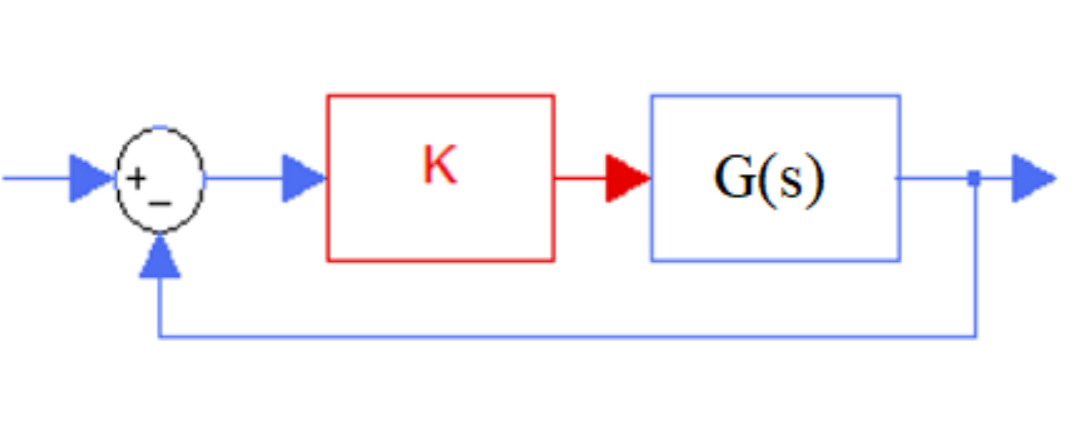
\includegraphics[scale=0.55]{control/Capture.PNG}
\end{figure}

\begin{figure}[h!]
\caption{Descripción gráfica de un controlador PID. Tomado de \cite{wiki:PID}\label{fig:PID}}
  \centering
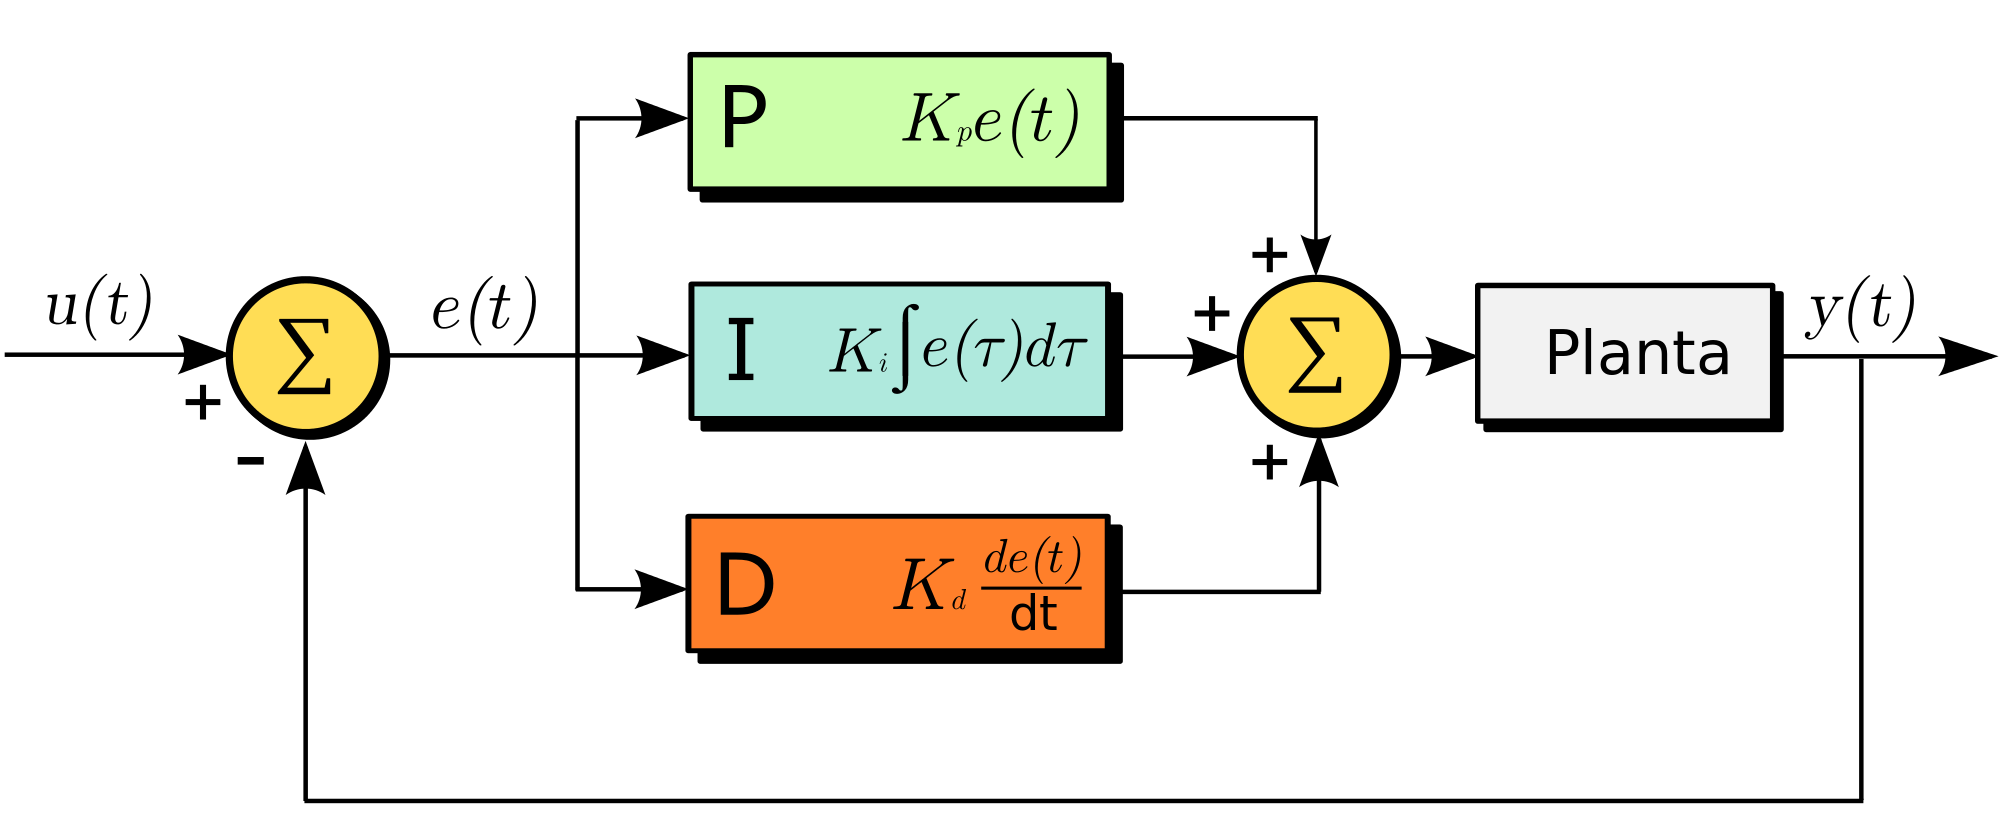
\includegraphics[scale=0.12]{control/Controlador_pid_svg.png}
\end{figure}

\subsection{Análisis control para $G_2$}
Primero, se analiza la posibilidad de aplicar a $G_2$ un controlador estático. Para ello, el paso inicial es ver el lugar de las raíces de $G_2$ (ver Figura \ref{fig:rlocusG2}). Se observa que a medida que se aumenta k, los polos conjugados se  vuelven inestables y el polo real tiende a ser menos dominante. Se define como polos dominantes aquellos que se encuentran más cerca al eje de las ordenadas. Por lo que se deduce que el valor óptimo para $k$ es 0, en otras palabras, no es recomendable implementar un controlador estático a $G_2$, éste sólo inestabilizaría el sistema.\\

\begin{figure}[h!]
\caption{Lugar de las raíces para $G_2$.\label{fig:rlocusG2}}
  \centering
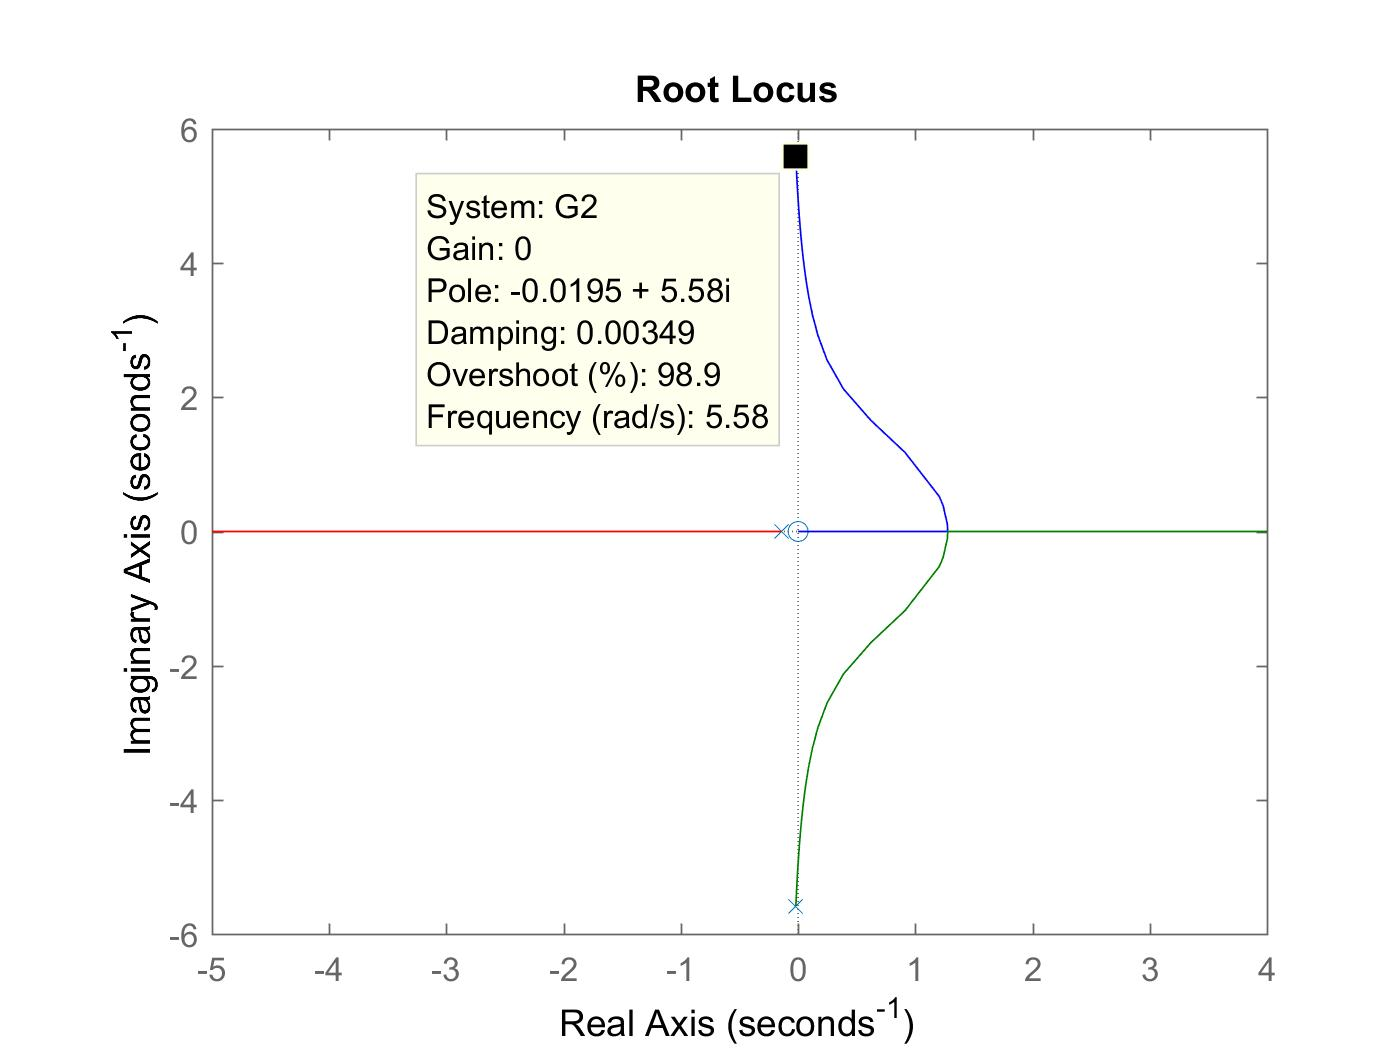
\includegraphics[scale=0.18]{control/k_G2.jpg}
\end{figure}

Ahora, dada la ineficacia de un controlador estático, se observa la posibilidad de aplicar un controlador PID. La Ecuación (\ref{eq:PID}) se puede rescribir como $$G_c(s) = \dfrac{K_D}{s}\bigg(s^2+\dfrac{K_P}{K_D}s+\dfrac{K_I}{K_D}\bigg)$$
Luego, se fijan valores para los coeficientes del segundo factor o el polinomio factorizado de segundo orden. Los valores dados son
$$\dfrac{K_P}{K_D} = 0.0389 \qquad \textnormal{y} \qquad \dfrac{K_I}{K_D} = 31.1763$$
que corresponden a sumar y multiplicar el inverso aditivo de los únicos dos polos conjugados de $G_2$. La finalidad de esta asignación es la eliminación de dichos polos como se verá a continuación. Para mirar como $K_D$ afecta a los polos del sistema, se multiplican $G_c$, con los valores fijados y dejando a un lado $K_D$, y $G_2$, resultando
$$G_{2c} = \dfrac{(s^2+0.0389s+31.1763)(-4.545 s)}{s(s^3 + 0.1818 s^2 + 31.18 s + 4.455)}$$
$$G_{2c} =  \dfrac{-4.545 s}{s^2 + 0.1429 s}$$\\

En la Figura \ref{fig:rlocusG2PID} se muestra el lugar de las raíces para $G_{2c}$ según el valor de $K_D$. Se podría llegar aplicar un controlador PID, pero no se considera de gran aporte. En conclusión, tampoco se recomienda la implementación de un controlador PID para $G_2$. La ineficacia de dichos controladores puede deberse a que $G_2$ es estable. 

\begin{figure}[h!]
\caption{Lugar de las raíces para $G_{2c}$ según $K_D$.\label{fig:rlocusG2PID}}
  \centering
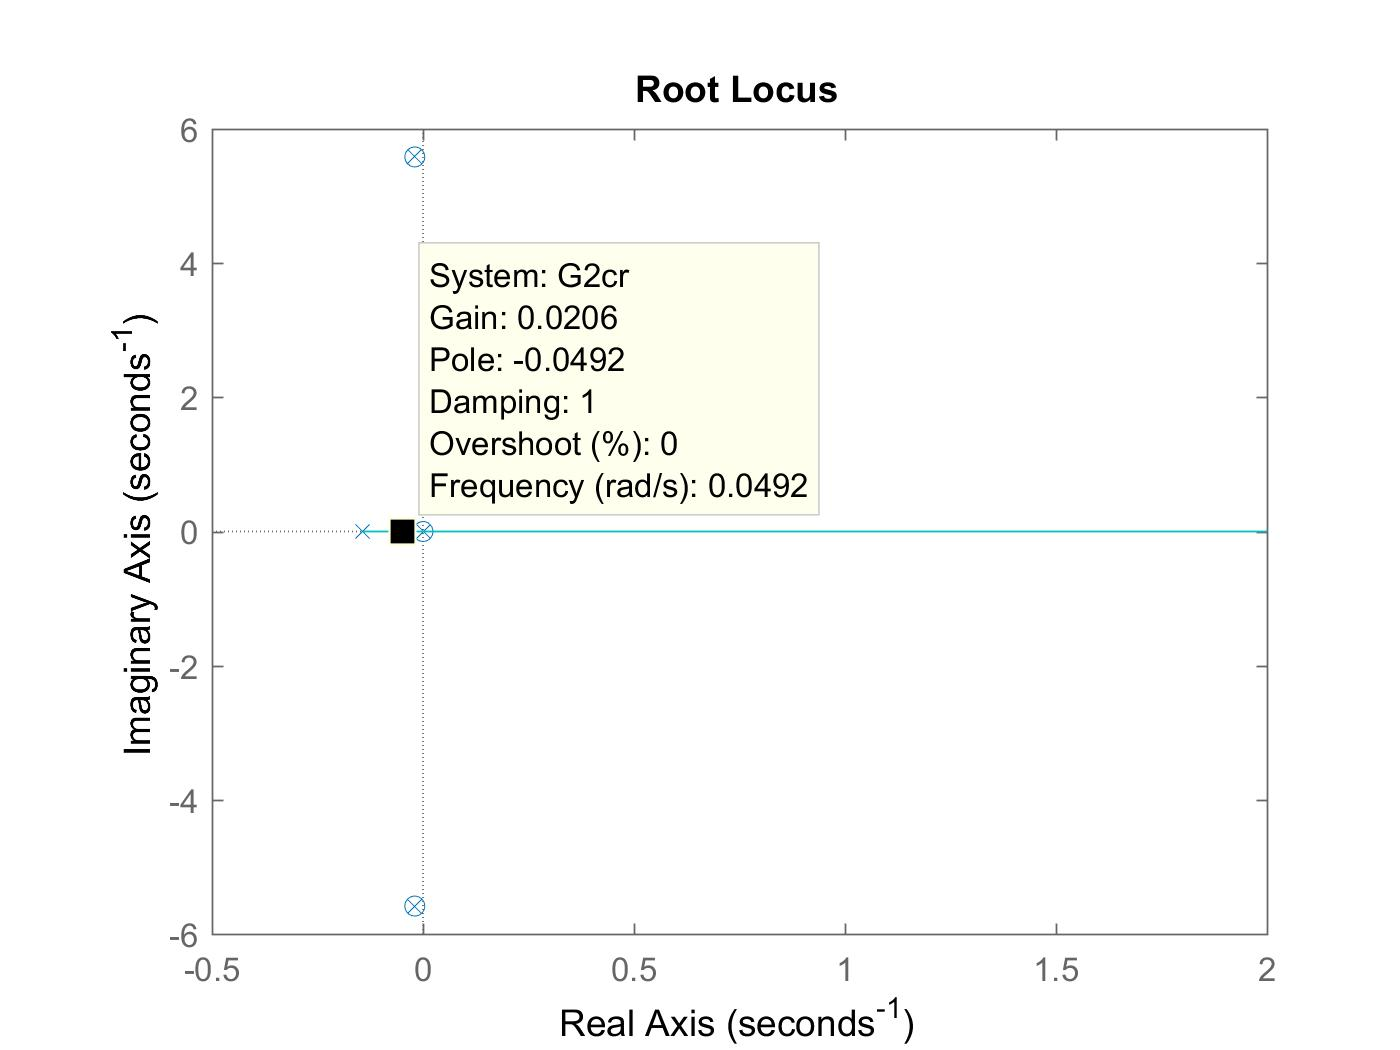
\includegraphics[scale=0.18]{control/PID_G2.jpg}
\end{figure}

\subsection{Análisis control para $G_1$}
Para el análisis de control de $G_1$ sólo se estudia la posibilidad de introducir un controlador estático. En próximas entregas se analizará la oportunidad de implementar un controlador PID. En la Figura \ref{fig:rlocusG1} se muestra el lugar de las raíces de $G_1$. Dada la posibilidad de mover el polo que se encuentra en (0,0) y que la estabilidad del sistema no se deteriora, sino que mejora, se decide aplicar un controlador estático con $k=0.00357$.\\   

\begin{figure}[h!]
\caption{Lugar de las raíces para $G_1$.\label{fig:rlocusG1}}
  \centering
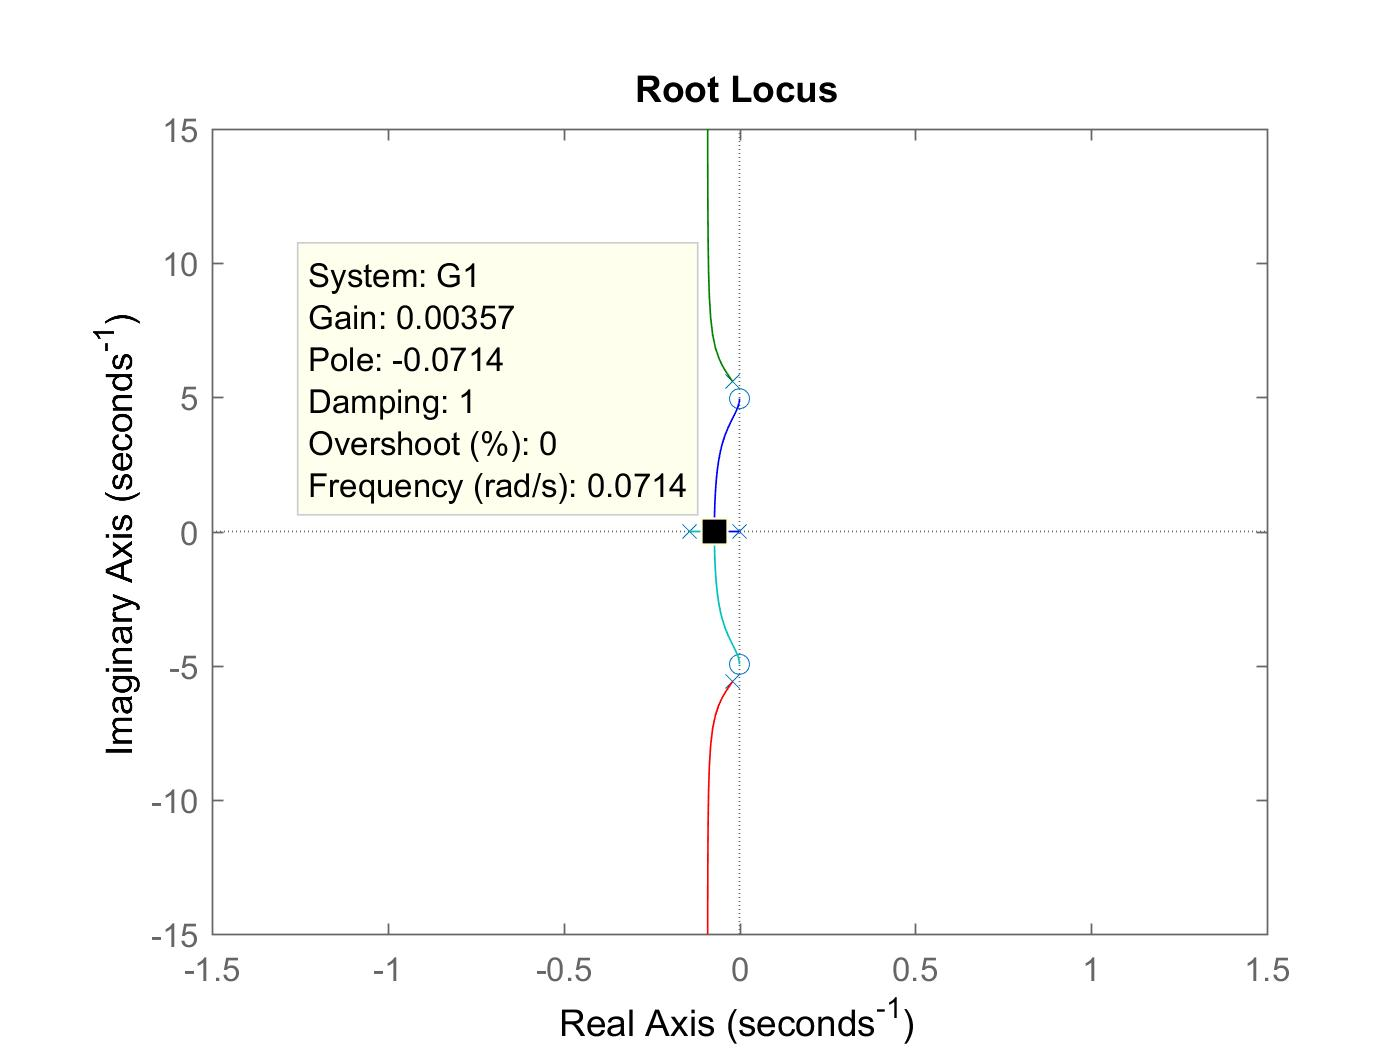
\includegraphics[scale=0.18]{control/k_G1.jpg}
\end{figure}

La función de transferencia en lazo cerrado para un controlador estático se calcula como $G_c = \dfrac{kG}{1+kG}$ dando como resultado
\\

\scalebox{0.75}{$G_c = \dfrac{0.006491 s^6 + 0.00118 s^5 + 0.3614 s^4 + 0.05783 s^3 + 4.959 s^2 + 0.7084 s}{ s^8 + 0.3636 s^7 + 62.4 s^6 + 20.25 s^5 + 974.3 s^4 + 277.9 s^3 + 24.8 s^2 + 0.7084 s}$}\\

Los polos, ceros y ganancia se especifican en el Cuadro \ref{tab: pzg tf1e}. Se observa que la función de transferencia para la salida $y_1$ aumenta su orden, teniendo más polos estables y continúa teniendo un polo en (0,0), haciendo que se siga considerando críticamente estable. A pesar de ello, la estabilidad mejora notablemente, como se puede verificar en la Figura \ref{fig:stepGc1}, presentándose convergencia en la respuesta temporal al escalón unitario, situación que ocurría antes de implementar el controlador.  

\begin{table}[!h]
\centering
\caption{Polos, ceros y ganancia de la función de transferencia $G1$ en lazo cerrado con controlador estático}
\label{tab: pzg tf1e}
\begin{tabular}{@{}lccc@{}}
\toprule
                  & Polos & Ceros             & Ganancia          \\ \midrule
\multirow{8}{*}{$G_1$} & 0 & 0 & 0.006491 \\
                       &   -0.0195 + 5.5837i      &     -0.0195 + 5.5835i      &         \\
                       &   -0.0195 - 5.5837i     &    -0.0195 - 5.5835i       &         \\
                       &   -0.0195 + 5.5837i      &   4.9497i        &         \\
                       &   -0.0195 - 5.5837i      &    - 4.9497i       &         \\
                       & -0.1429      &     -0.1429      &         \\
                       & -0.0729     &           &         \\
                       & -0.0699     &           &         \\
                       \bottomrule
\end{tabular}
\end{table}

\begin{figure}[h!]
\caption{Respuesta al escalón unitario para la función de transferencia $G_1$ en lazo cerrado con controlador estático.\label{fig:stepGc1}}
  \centering
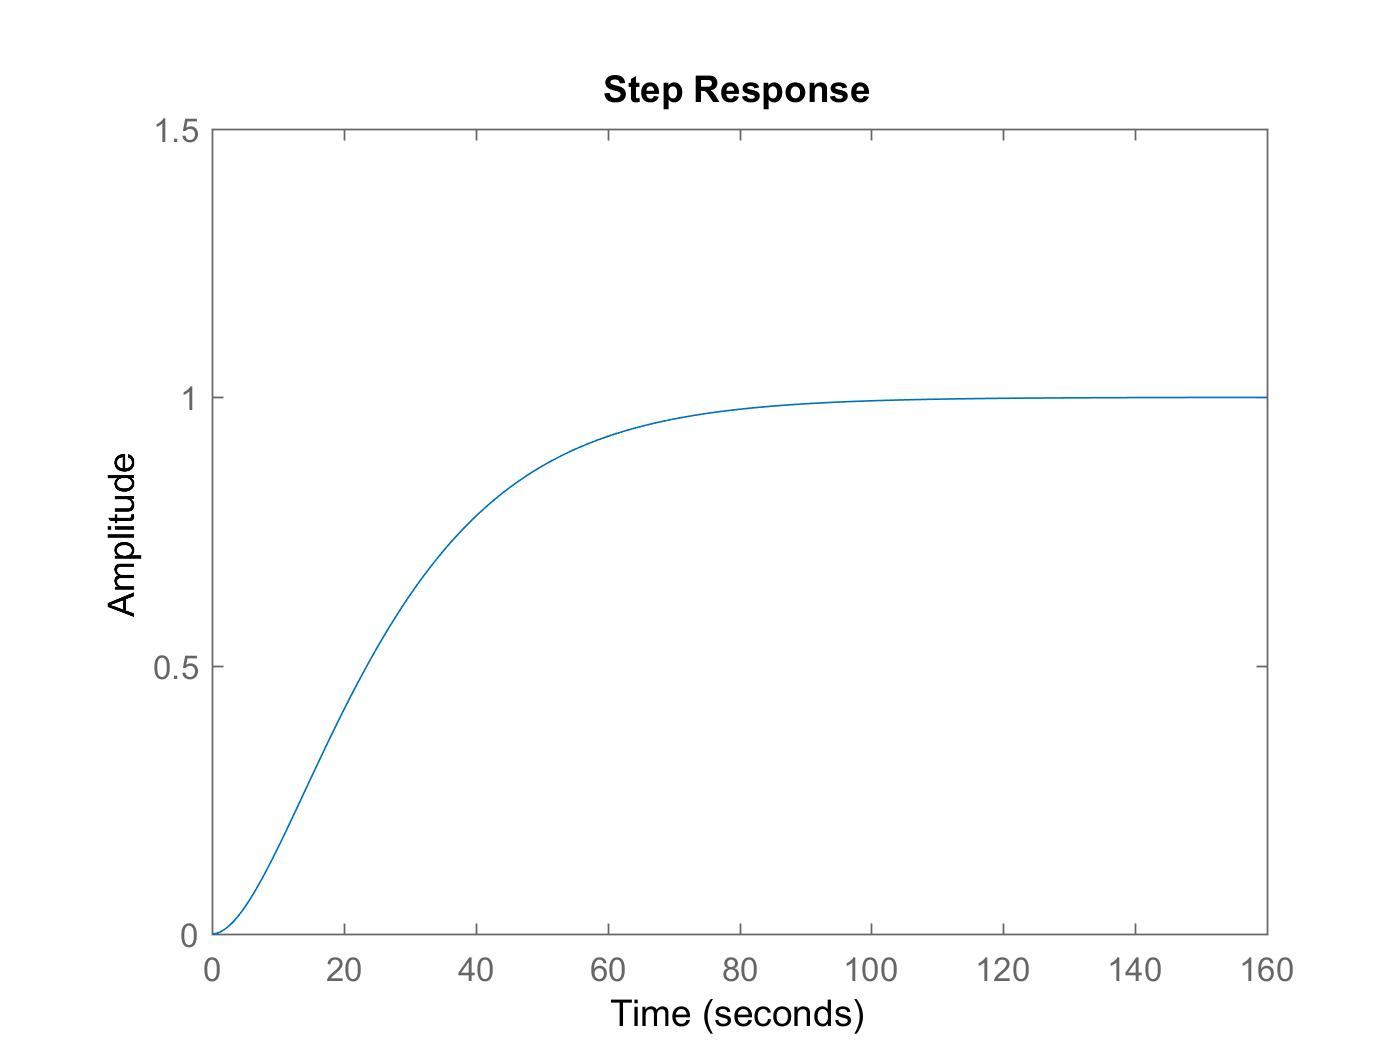
\includegraphics[scale=0.18]{control/step_Gc1.jpg}
\end{figure}
\vspace{20pt}
\section{Routh-Hurwitz y Jury}
Esta sección se encuentra anexada al final del documento. La razón por la que se encuentra anexa es debido la forma en cómo desarrolla, con un procedimiendo matemático detallado.

\section{Conclusiones}
El péndulo invertido es un modelo no lineal que posee múltiples puntos de equilibrio, entre ellos $X_0=0$ y $U_0=0$. Diferentes análisis de estabilidad muestran que el sistema en dicho punto es críticamente estable. Entre estos análisis se encuentran la definición de estabilidad con base en los valores propios de la matriz A del modelo linealizado en el punto de equilibrio mencionado, la ubicación de los polos de la función de transferencia y el método de Routh-Hurwitz. La salida que hace al modelo críticamente estable es $y_1$. Lo anterior se observa en las diferentes respuestas temporales de dicha salida: para señales de entrada no oscilantes y con pendiente monótonamente creciente o decreciente, como el escalón unitario y la función sierra, la respuesta temporal no converge; mientras que, para señales de comportamiento sinusoidal o no constantes, como el impulso unitario, tiende a converger a un valor.\\

La reducción de orden de la función de transferencia del sistema hace que las respuestas temporales de la salida $y_2$ pierdan su carácter oscilatorio, debido a que al realizar la reducción sólo quedan polos reales, desapareciendo los polos complejos conjugados. A pesar de ello, el carácter críticamente estable del sistema se conserva. De igual forma ocurre cuando se discretiza el sistema. En los tres tiempos de muestreo propuestos $0.21, 0.73,1.26$ la estabilidad del sistema y la forma de las respuestas temporales se conservan. Se comprueba que a menor tiempo de muestro, más se asemejan las funciones de transferencia en tiempo continuo y en tiempo discreto.\\


Por último, para la función de transferencia asociada a la salida $y_2$, ni la aplicación de un controlador estático ni de un controlador PID muestra ser beneficiosa; por el contrario, tienden a desestabilizar la planta. Lo que no pasa con función de transferencia relacionada a la salida $y_1$, la cual al implementarse un controlador estático mejora su estabilidad. Esto se observa notablemente en la convergencia en la respuesta temporal a la señal escalón unitario.  


\bibliography{ref}
\bibliographystyle{IEEEtran}

\newpage
\subsection{Espacios de estados generalizados}
\[
  \bm{x} =
  \begin{pmatrix}
    x_1\\
    x_2\\
    x_3\\
    x_4
  \end{pmatrix}
  \in \mathbb{R}^{4 \times 1} \quad
  \bm{u} = u \in \mathbb{R}^{1 \times 1} \quad
  \bm{y} =
  \begin{pmatrix}
    y_1\\
    y_2
  \end{pmatrix}
  \in \mathbb{R}^{2 \times 1}
\]
\[
  \bm{A} =
  \begin{pmatrix}
    0 & 1    & 0   & 0 \\
    0 & -c_2 & c_1  & 0 \\
    0 & 0    & 0   & 1 \\
    0 & c_4  & c_3  & 0
  \end{pmatrix}
  \in \mathbb{R}^{4 \times 4}
  \quad
  \bm{B} =
  \begin{pmatrix}
    0   \\
    c_5 \\
    0   \\
    -c_6
  \end{pmatrix}
  \in \mathbb{R}^{4 \times 1}
\]
\[
  \bm{C} =
  \begin{pmatrix}
    1 & 0 & 0 & 0 \\
    0 & 0 & 1 & 0
  \end{pmatrix}
  \in \mathbb{R}^{2 \times 4} \quad
  \bm{D} = \bm{0} \in \mathbb{R}^{2 \times 1}
\]

donde

\[ c_1 = \frac{m^2 g l^2}{\alpha} \quad c_2 = \frac{(I + m l^2) b}{\alpha} \quad
   c_3 = \frac{m g l (M + m)}{\alpha} \]
\[ c_4 = \frac{m l b}{\alpha} \quad c_5 = \frac{I + m l^2}{\alpha} \quad
   c_6 = \frac{m l}{\alpha} \]
\[\alpha = I(M + m) + m M l^2\]
\\
Para los valores definidos de los parámetros obtenemos que las constantes $c_i$
toman los siguientes valores.
\[ c_1 = 2.6745 \quad c_2 = 0.1818 \quad c_3 = 31.2030 \]
\[ c_4 = 0.4545 \quad c_5 = 1.8182 \quad c_6 = 4.5455 \]


\subsection{Funciones de transferencia generalizadas}
Para hallar la matriz de funciones de transferencia debemos utilizar el metodo
expuesto por~\cite{dorf67}, el cual la define como
\[ \vb*{G}(s) = \vb*{C} (s \vb*{I} - \vb*{A})^{-1} \vb*{B} - \vb*{D}. \]
\\

Para esto definamos inicialmente la matriz
\[ s \bm{I} - \bm{A} =
  \begin{pmatrix}
     s & -1 & 0 & 0 \\
     0 & c_2+s & -c_1 & 0 \\
     0 & 0 & s & -1 \\
     0 & -c_4 & c_3 & s \\
  \end{pmatrix},
  \] que tiene como determinante
\begin{align*}
  p = p(s)
  &= \det(s \bm{I} - \bm{A})\\
  &= s [s^2 (s + c_2) - (c_1 c_4 - (s + c_2) c_3)]\\
  &= s [(s + c_2) (s^2 + c_3) - c_1 c_4]\\
  &= s [s^3 + c_2 s^2 + c_3 s + (c_2 c_3 - c_1 c_4)].
\end{align*}
Con la matriz y el determinante podemos hallar la inversa de la siguienta manera
\[ (s \bm{I} - \bm{A})^{-1} = \frac{1}{p(s)} \operatorname{adj} (s \bm{I} - \bm{A})^{-1} \]
Donde la inversa de $(s \bm{I} - \bm{A})^{-1}$ está dada por:
\[ \frac{1}{p}
  \begin{pmatrix}
    p s^{-1} & s^2+c_3 & c_1 s & c_1 \\
    0 & s^3+ c_3 s & c_{1} s^2 & c_{1} s \\
    0 & c_{4} s & s^3+c_{2} s^2 & s^2+c_{2} s \\
    0 & c_{4} s^2 & -c_{3} s^2-c_{2} c_{3} s+c_{1} c_{4} s & s^3+c_{2} s^2 \\
  \end{pmatrix}
\]
\\

Lo que nos permite hallar la matriz de funciones de transferencia

\begin{align*}
  C (s \bm{I} - \bm{A})^{-1} B
  &= \frac{1}{p(s)}
    \begin{pmatrix}
      c_5 s^2 - (c_1 c_6 - c_3 c_5)\\
      s (-c_6 s + (c_4 c_5 - c_2 c_6))
    \end{pmatrix}\\
  &=
    \begin{pmatrix}
      \dfrac{c_5 s^2 - (c_1 c_6 - c_3 c_5)}{s^4 + c_2 s^3 + c_3 s^2 + (c_2 c_3 - c_1 c_4)s}\\
      \dfrac{-c_6 s + (c_4 c_5 - c_2 c_6)}{s^3 + c_2 s^2 + c_3 s + (c_2 c_3 - c_1 c_4)}
    \end{pmatrix}
\end{align*}
\\

Reemplazando los valores de $c_i$ obtenemos que:
\[ \vb*{G}(s) =
  \begin{pmatrix}
    \dfrac{1.818 s^2 + 44.58}{s^4 + 0.1818 s^3 + 31.2 s^2 + 4.458 s}\\
    \dfrac{-4.545 s}{s^3 + 0.1818 s^2 + 31.2 s + 4.458}
  \end{pmatrix}.
\]

\subsection{Estabilidad}
\subsubsection{Estabilidad del modelo}
Análisis de estabilidad lineal en tiempo continuo en el punto de operación seleccionado. El polinomio característico está dado por
\begin{equation}
  \label{eq:polcar}
  \begin{split}
  p(s)
  &= s^4 + 0.1818 s^3 + 31.2030 s^2 + 4.4576 s\\
  &= s (s^3 + 0.1818 s^2 + 31.2030 s + 4.4576) \\
\end{split}
\end{equation}
\textbf{}

Aplicando el método de Routh-Hurwitz al polinomio sin $\frac{p(s)}{s}$ obtenemos que
\[
  \begin{array}{c|cc}
    s^3 & 1 & 31.2030\\
    s^2 & 0.1818 & 4.4576\\
    s^1 & 6.6864 &\\
    s^0 & 4.4576 &
  \end{array}
\]
\\

Si se quisiera determinar la estabilidad por el método indirecto de Lyapunov\cite{Murray:1994:MIR:561828}, se obtendría un valor propio en cero lo cual no permite concluir.\\

Para hacerlo de forma general, es importante notar que el denominador para la función de transferencia asociada a la posición del carro es \[ p(s) \] mientras que, el denominador para la función de transferencia asociada al ángulo del péndulo es \[ \frac{p(s)}{s} \]

Para determinar la estabilidad de cada función de transferencia en lazo abierto por separado es necesario mirar la ubicación de los polos. El denominador de la función de transferencia de la posición del carro es \[ s^4 + c_2 s^3 + c_3 s^2 + (c_2 c_3 - c_1 c_4)s, \] función que no cumple las condiciones necesarias de Routh-Hurwitz debido que hay un $a_i = 0$.\\

Para la función de transferencia asociada al ángulo del péndulo tenemos que el denominador es \[ s^3 + c_2 s^2 + c_3 s + (c_2 c_3 - c_1 c_4). \] Una verificación inicial de las condiciones necesarias nos lleva a concluir que $c_2 > 0$, $c_3 > 0$, ambas por definicion. Adicionalmente tenemos que
\begin{align*}
  c_2 c_3 - c_1 c_4
  &= \frac{(I + ml^2)b}{\alpha} \frac{mgl(M + m)}{\alpha} - \frac{m^2 g l^2}{\alpha} \frac{mlb}{\alpha}\\
  &= \frac{mgl}{\alpha} [(I + m l^2) (M + m) - m^2 l ^2] b\\
  &= \frac{mgl}{\alpha} [I(M + m) + m M l^2] b\\
  &> 0.
\end{align*}

Como las condiciones necesarias son satisfechas, es necesario plantear el arreglo de Routh-Hurwitz.

\[
  \begin{array}{c|cc}
    s^3 & 1 & c_3\\
    s^2 & c_2 & (c_2 c_3 - c_1 c_4)\\
    s^1 & \dfrac{c_1 c_4}{c_2} &\\
    s^0 & c_2 c_3 - c_1 c_4 &
  \end{array}
\]

El arreglo de Routh-Hurwitz, en este caso, nos plantea una condición adicional, es decir, \[ \frac{c_1 c_4}{c_2} > 0, \] condición que se cumple debido a que $c_i > 0 \ \forall i$.\\

\subsubsection{Rango de estabilidad para un parámetro}
Se toma inicialmente el parámetro $b$ ---coeficiente de fricción del carro--- para determinar la estabilidad del sistema en función de éste. Para esto, se definen unas constantes auxiliares
\[ c_2^* = \frac{I + m l^2}{\alpha} \implies c_2 = c_2^* b \]
\[ c_4^* = \frac{m l}{\alpha} \implies c_4 = c_4^* b \]

En este caso, el denominador de la función de transferencia de la posición del carro es \[ s^4 + c_2^* b s^3 + c_3 s^2 + (c_2^* c_3 - c_1 c_4^*) b s, \] que, al igual que el caso anterior, no cumple las condiciones necesarias de Routh-Hurwitz.\\

Para la función de transferencia asociada al ángulo del péndulo se tiene que el denominador es \[ s^3 + c_2^* b s^2 + c_3 s + (c_2^* c_3 - c_1 c_4^*) b. \] Un análisis similar permite determinar que las condiciones necesarias se cumplen y que para las condiciones suficientes se necesita que \[ \frac{c_1 c_4*}{c_2} > 0, \] condición que se sigue cumpliendo debido a que $c_4^* > 0$.\\

Se puede concluir que para $b \in \mathbb{R}^+$ el sistema es estable.\\


Se toma ahora el parámetro $g$ ---gravedad--- para determinar la estabilidad del sistema en función de éste. Para esto, nuevamente, se definen unas constantes auxiliares
\[ c_1^* = \frac{m^2 l^2}{\alpha} \implies c_1 = c_1^* g \]
\[ c_3^* = \frac{m l (M + m)}{\alpha} \implies c_3 = c_3^* g \]

En este caso, el denominador de la función de transferencia de la posición del carro es
\[ s^4 + c_2 s^3 + c_3^* g s^2 + (c_2 c_3^* - c_1^* c_4) g s, \] que, al igual que el caso
anterior, no cumple las condiciones necesarias de Routh-Hurwitz.\\

Para la función de transferencia asociada al ángulo del péndulo se tiene que el
denominador es \[ s^3 + c_2 s^2 + c_3^* s + (c_2 c_3^* - c_1^* c_4) g. \]
Un análisis similar permite determinar que las condiciones necesarias se
cumplen y que para las condiciones suficientes se necesita que
\[ \frac{c_1^* c_4}{c_2} > 0, \] condición que se sigue cumpliendo debido a que $c_1^* > 0$.\\

Se puede concluir que para $g \in \mathbb{R}^+$ el sistema es estable.

\subsection{Estabilidad del modelo discretizado}
Para analizar la estabilidad del sistema discretizado, se emplea el método de Jury, un método popular, equivalente en discreto al método de Routh-Hurwitz (trabajado anteriormente). Se utiliza para determinar
el número de raíces de un polinomio que se encuentran dentro del circulo unitario.\\


Se considera inicialmente la función de transferencia discreta, presentada anteriormente
\[
\dfrac{0.03866 z^3 - 0.001061 z^2 - 6.895e^{-05} z + 0.03817}{z^4 - 2.743 z^3 + 3.484 z^2 - 2.704 z + 0.9625}\]
\[
\dfrac{-0.08809 z^2 + 0.001042 z + 0.08705}{z^3 - 1.743 z^2 + 1.741 z - 0.9625}
\]
Ahora veamos los polinomios característicos de cada una de ellas,
\[
P_1(z) = {z^4 - 2.743 z^3 + 3.484 z^2 - 2.704 z + 0.9625}\]
\[
P_2(z) = {z^3 - 1.743 z^2 + 1.741 z - 0.9625}
\]

Veamos primero si $P_1$ cumple las condiciones necesarias para la estabilidad.
\begin{enumerate}
\item $P_1(1) > 0 \implies 1^4 - 2.743 1^3 + 3.484 1^2 - 2.704 1 + 0.9625 = 0 \ngtr 0$
\item $(-1)^nP(-1)>0 \implies (-1)^4 - 2.743 (-1)^3 + 3.484 (-1)^2 + 2.704 + 0.9625 = 10.8935 > 0$
\item $|a_n| < a_0 \implies 0.9625 < 1$ 
\end{enumerate}
\textbf{}

Veamos ahora si $P_2$ cumple las condiciones necesarias para la estabilidad
\begin{enumerate}
\item $P_2(1) > 0 \implies 1^3 - 1.743 1^2 + 1.741 - 0.9625 = 0.0355 > 0$
\item $(-1)^nP(-1)>0 \implies (-1)^3 - 1.743 (-1)^2 - 1.741 - 0.9625 = -5.4465 < 0$
\item $|a_n| < a_0 \implies 0.9625 < 1$ 
\end{enumerate}
\textbf{}

Inicialmente, se puede decir que $P_2$ cumple las condiciones necesarias para la estabilidad, lo cual se relaciona fuermente con los resultados presentados anteriormente. Por otro lado, de $P_1$ se puede decir que el sistema no es estable, dado que no cumple la primera condición necesaria; sin embargo, anteriormente se había llegado a la conclusión de que dicho sistema es críticamente estable, lo cual se puede deducir al ver que $P_1$ evaluado en 1 se hace 0. %%ahora, al momento de realizar los computos, tanto matlab como nosotros realizamos diferentes aproximaciones, las cuales pudieron desplazar ligeramente los polos del sistema, haciéndolo inestable. De esto podemos concluir que le método es bastante sensible a este tipo de modificaciones.%% %%No es verdad%%
\end{document}
